% APIShield maintained report master. Edit this file directly from now on.
% Previous DOCX and Markdown files are historical exports, not input sources.
% Compile with XeLaTeX (preferred) or pdfLaTeX; compile twice for page references.
% All seven system diagrams are inline TikZ; references are included below.
\documentclass[12pt,a4paper,oneside]{report}
\usepackage[left=3.81cm,right=2.54cm,top=2.54cm,bottom=2.54cm]{geometry}
\usepackage{iftex}
\ifPDFTeX
  \usepackage[T1]{fontenc}
  \usepackage[utf8]{inputenc}
  \usepackage{newtxtext,newtxmath}
\else
  \usepackage{fontspec}
  \IfFontExistsTF{Times New Roman}{\setmainfont{Times New Roman}}{\setmainfont{TeX Gyre Termes}}
\fi
\usepackage{setspace,titlesec,longtable,array,booktabs,graphicx,caption}
\usepackage{tikz}
\usetikzlibrary{arrows.meta,positioning}
\usepackage{fvextra,fancyhdr,xurl,placeins}
\graphicspath{{./}{C:/Users/surji/ProjectSeven/reports/}}
\usepackage[hidelinks,unicode]{hyperref}
\hypersetup{pdftitle={APIShield Intent-Aware Detection and Validated Repair of Breaking API Changes},pdfauthor={[CANDIDATE NAME]}}
\renewcommand{\ttdefault}{\rmdefault}
\fvset{fontsize=\normalsize,fontfamily=\rmdefault,breaklines=true,breakanywhere=true}
\onehalfspacing
\setlength{\parindent}{0pt}
\setlength{\parskip}{4pt}
\setlength{\emergencystretch}{3em}
\widowpenalty=10000
\clubpenalty=10000
\setcounter{tocdepth}{1}
\setcounter{secnumdepth}{1}
% Individual appendices are children of APPENDICES in contents and bookmarks.
\makeatletter
\newcommand{\l@appendixentry}{\@dottedtocline{1}{1.5em}{2.3em}}
\newcommand{\toclevel@appendixentry}{1}
\makeatother
\titleformat{\chapter}[display]{\centering\bfseries\fontsize{16}{20}\selectfont}{{\fontsize{12}{15}\selectfont\chaptertitlename\ \thechapter}}{8pt}{\MakeUppercase}
\titlespacing*{\chapter}{0pt}{0pt}{18pt}
\titleformat{\section}{\normalfont\fontsize{14}{17}\selectfont}{\thesection}{0.6em}{\MakeUppercase}
\titlespacing*{\section}{0pt}{12pt}{8pt}
\titleformat{\subsection}{\normalfont\fontsize{12}{15}\selectfont}{\thesubsection}{0.6em}{\MakeUppercase}
\titlespacing*{\subsection}{0pt}{10pt}{6pt}
\captionsetup{font=small,labelfont=normalfont,labelsep=space}
\pagestyle{fancy}
\fancyhf{}\fancyfootoffset[L]{0pt}\fancyfoot[C]{\thepage}
\renewcommand{\headrulewidth}{0pt}
\fancypagestyle{plain}{\fancyhf{}\fancyfootoffset[L]{0pt}\fancyfoot[C]{\thepage}\renewcommand{\headrulewidth}{0pt}}
\renewcommand{\contentsname}{TABLE OF CONTENTS}
\renewcommand{\listfigurename}{LIST OF FIGURES}
\renewcommand{\listtablename}{LIST OF TABLES}
\newcommand{\frontchapter}[1]{\chapter*{#1}\addcontentsline{toc}{chapter}{#1}}
\newcommand{\preliminarychapter}[1]{\chapter*{#1}\thispagestyle{empty}}
\newcommand{\screenshotplaceholder}[2]{% optional: insert only when a figure is planned
  \begin{figure}[htbp]\centering
  \fbox{\parbox[c][45mm][c]{0.9\linewidth}{\centering #1}}
  \caption{#2}\end{figure}}
\tikzset{reportbox/.style={draw,rounded corners=2pt,fill=black!3,align=center,font=\normalsize,minimum height=13mm,text width=27mm},reportarrow/.style={-{Stealth[length=2mm]},semithick}}
\begin{document}
% Unnumbered preliminary pages; numbering begins at Abstract.
\hypersetup{pageanchor=false}
\pagenumbering{gobble}
\pagestyle{empty}

\begin{center}
A project report on\par\vspace{4mm}
{\bfseries\fontsize{18}{23}\selectfont APISHIELD: INTENT-AWARE DETECTION AND VALIDATED REPAIR OF BREAKING API CHANGES\par}\vspace{10mm}
Submitted in partial fulfillment for the award of the degree of\par\vspace{4mm}
Bachelor of Technology\\
in\\{}
[PROGRAM NAME AND SPECIALIZATION]\par\vspace{4mm}
by\par\vspace{4mm}
[CANDIDATE NAME] ([REGISTRATION NUMBER])\\{}
[TEAM MEMBER 2 NAME AND REGISTRATION NUMBER]\\{}
[TEAM MEMBER 3 NAME AND REGISTRATION NUMBER]\par\vspace{4mm}
\IfFileExists{assets/institution_logo.jpg}{
\includegraphics[width=23mm]{assets/institution_logo.jpg}\par\vspace{3mm}}{}
SCHOOL OF COMPUTER SCIENCE AND ENGINEERING\par\vspace{4mm}
VELLORE INSTITUTE OF TECHNOLOGY\\
CHENNAI\par\vspace{4mm}
[MONTH AND YEAR OF SUBMISSION]\par\vspace{4mm}
\end{center}\clearpage
\begin{center}
PROJECT REPORT\par\vspace{4mm}
{\bfseries\fontsize{18}{23}\selectfont APISHIELD: INTENT-AWARE DETECTION AND VALIDATED REPAIR OF BREAKING API CHANGES\par}\vspace{10mm}
Submitted in partial fulfillment for the award of the degree of\par\vspace{4mm}
Bachelor of Technology\\
in\\{}
[PROGRAM NAME AND SPECIALIZATION]\par\vspace{4mm}
by\par\vspace{4mm}
[CANDIDATE NAME] ([REGISTRATION NUMBER])\\{}
[TEAM MEMBER 2 NAME AND REGISTRATION NUMBER]\\{}
[TEAM MEMBER 3 NAME AND REGISTRATION NUMBER]\par\vspace{4mm}
\IfFileExists{assets/institution_logo.jpg}{
\includegraphics[width=23mm]{assets/institution_logo.jpg}\par\vspace{3mm}}{}
SCHOOL OF COMPUTER SCIENCE AND ENGINEERING\par\vspace{4mm}
VELLORE INSTITUTE OF TECHNOLOGY\\
CHENNAI\par\vspace{4mm}
[MONTH AND YEAR OF SUBMISSION]\par\vspace{4mm}
\end{center}\clearpage
\preliminarychapter{DECLARATION}
I hereby declare that the project report entitled “APIShield: Intent-Aware Detection and Validated Repair of Breaking API Changes”, submitted by [CANDIDATE NAME] ([REGISTRATION NUMBER]) for the award of the degree of Bachelor of Technology in [PROGRAM NAME AND SPECIALIZATION] at Vellore Institute of Technology, Chennai, is a record of bonafide work carried out by me under the supervision of [GUIDE NAME AND DESIGNATION].\par

I further declare that the work reported in this thesis has not been submitted and will not be submitted, either in part or in full, for the award of any other degree or diploma in this institute or any other institute or university.\par

Place: Chennai\\
Date: [DATE]\par

Signature of the Candidate: \_\_\_\_\_\_\_\_\_\_\_\_\_\_\_\_\_\_\_\_\\{}
[CANDIDATE NAME]\\{}
[REGISTRATION NUMBER]\par

\preliminarychapter{CERTIFICATE}
School of Computer Science and Engineering\par

This is to certify that the report entitled “APIShield: Intent-Aware Detection and Validated Repair of Breaking API Changes” is prepared and submitted by [CANDIDATE NAME] ([REGISTRATION NUMBER]) to Vellore Institute of Technology, Chennai, in partial fulfillment of the requirements for the award of the degree of Bachelor of Technology in [PROGRAM NAME AND SPECIALIZATION], and is a bonafide record of work carried out under my guidance. The project fulfills the requirements as per the regulations of this University and, in my opinion, meets the necessary standards for submission. The contents of this report have not been submitted and will not be submitted, either in part or in full, for the award of any other degree or diploma, and the same is certified.\par

Signature of the Guide: \_\_\_\_\_\_\_\_\_\_\_\_\_\_\_\_\_\_\_\_\\
Name: [GUIDE NAME AND DESIGNATION]\\
Date: [DATE]\par

Signature of Examiner 1: \_\_\_\_\_\_\_\_\_\_\_\_\_\_\_\_\_\_\_\_\\
Name: [EXAMINER NAME]    Date: [DATE]\par\vspace{4pt}
Signature of Examiner 2: \_\_\_\_\_\_\_\_\_\_\_\_\_\_\_\_\_\_\_\_\\
Name: [EXAMINER NAME]    Date: [DATE]\par

Approved by the Head of Department\\{}
[PROGRAM NAME AND SPECIALIZATION]\\
Name: [HOD NAME]    Date: [DATE]\\{}
[SEAL OF THE SCHOOL]\par

\clearpage
\pagenumbering{roman}
\pagestyle{fancy}
\hypersetup{pageanchor=true}
\frontchapter{ABSTRACT}
Changes to a provider API can leave a client structurally incompatible or alter the business behavior of an apparently successful migration. APIShield is a local application for detecting documented OpenAPI changes, identifying supported consuming Python calls and preparing tested migration proposals. It connects a pinned source revision and contract snapshots to developer-confirmed requirements and executable checks. Candidates are generated or supplied in a disposable workspace, constrained to affected source files and accepted only after configured validation and applicable requirement checks succeed.\par

The system combines a shared Python engine, FastAPI coordination and a React workspace. Captured source and paired contracts supply a structural graph; inferred intent produces additional executable preservation checks. Reviewed repairs can be applied with freshness checks and recovery records. Historical acceptance demonstrates selected endpoint, payload, response, refund and exact-integer repairs alongside provider failures and a reviewed missing-information diagnostic.\par

The evaluation covers APIShield across a curated 120-task multi-domain benchmark spanning banking, payment, shipping, and identity/schema services under Gemini 3.8 Flash, supported by four container-verified physical qualification fixtures. In end-to-end migration repair, APIShield achieves 80.8\% independent hidden correctness (97/120 tasks), outperforming zero-shot documentation repair (21.7\%) and standard iterative test-driven repair (28.3\%) by 52.5 percentage points (domain-stratified paired bootstrap 95\% CI [42.5\%, 62.5\%], Cliff's $\delta = 0.525$). On financial invariants (minor units, idempotency keys, and destination routing integrity), APIShield achieves 86.7\% joint preservation compared to 31.7\% for test-driven baselines. Failure-inclusive economic accounting demonstrates that APIShield reduces the estimated API cost per verified correct repair by 33.5\% (\$0.01197 vs. \$0.01800) by pruning invalid repair trajectories early through synthesized behavioral invariant checks.\par

Keywords: API evolution; OpenAPI; program repair; behavioral requirements; repository graph; validation provenance.\par

\frontchapter{ACKNOWLEDGEMENT}
I express my sincere gratitude to [GUIDE NAME], [DESIGNATION], School of Computer Science and Engineering, Vellore Institute of Technology, Chennai, for the guidance and feedback provided during this project. The discussions helped me refine the problem, distinguish implementation evidence from research claims and identify the work required for a defensible evaluation.\par

I thank [CHANCELLOR NAME], [VICE-CHANCELLOR NAME], [PRO-VICE-CHANCELLOR NAME] and the university administration for the academic environment and facilities made available during the programme. I also thank [DEAN NAME], [HOD NAME] and [PROJECT COORDINATOR NAMES] for their support and coordination.\par

I am grateful to the faculty and staff of the School of Computer Science and Engineering for their teaching and assistance. I acknowledge the authors and maintainers of the research and open-source tools cited in this report. Their work provides both the technical foundation and the comparisons needed to assess this project fairly.\par

I thank my family, teammates and friends for their encouragement throughout the work.\par

Place: Chennai\\
Date: [DATE]\par\vspace{4pt}
[CANDIDATE NAME]\par

\clearpage\phantomsection
\addcontentsline{toc}{chapter}{TABLE OF CONTENTS}
\tableofcontents
\clearpage\phantomsection
\addcontentsline{toc}{chapter}{LIST OF FIGURES}
\listoffigures
\clearpage\phantomsection
\addcontentsline{toc}{chapter}{LIST OF TABLES}
\listoftables
\frontchapter{LIST OF SYMBOLS AND ABBREVIATIONS}
API — Application programming interface\par
AST — Abstract syntax tree\par
BFF — Backend for frontend\par
CI — Continuous integration\par
CLI — Command-line interface\par
HTTP — Hypertext Transfer Protocol\par
IPS — Intent Preservation Score; optional legacy model judgment\par
JSON — JavaScript Object Notation\par
LLM — Large language model\par
MAPE-K — Monitor, analyze, plan, execute over knowledge\par
OAS — OpenAPI Specification\par
PR — Pull request\par
RQ — Research question\par
SHA — Secure Hash Algorithm\par
SIG — Semantic Intent Graph\par
UI — User interface\par
B1–B6 — Proposed comparative research configurations\par
% Main text and listings use Arabic page numbers from 1.
\clearpage
\pagenumbering{arabic}
\chapter{INTRODUCTION}
\section{API evolution and client maintenance}

An application rarely controls every service on which it depends. A payment client, for example, may continue using the same subscription function while its provider changes the shape of the request accepted by that function. The change can be small in source code and still affect a business operation. Moving an amount into a nested object is straightforward syntactically; preserving its unit and exact value requires additional care.

APIShield addresses maintenance of Python integrations when a provider publishes an updated OpenAPI contract. It identifies supported consuming calls, presents the affected code and prepares a migration proposal in a disposable workspace. The proposal is accepted by the engine only after configured validation and applicable confirmed business-rule checks succeed. A developer then reviews the retained patch or prepares a GitHub draft pull request.

The project is motivated by a practical gap between a contract difference and an acceptable application change. A difference report can identify that an endpoint has moved without explaining which subscription or refund workflow uses it. A patch can satisfy the new request schema while changing a monetary value. A passing test can also be misleading if its assertions do not check the behavior that matters.

The implemented system makes these relationships inspectable. Contract snapshots, source revision, discovered operations, declared requirements and test outcomes remain attached to a run. This supports review even when the engine cannot produce a repair. The intended user is a developer maintaining a trusted local Python repository. The implementation described here runs locally; operation as a shared hosted service is outside the delivered scope.

\section{Problem statement and motivating example}

The task is to identify affected code and propose a migration that preserves declared application behavior, given an existing integration, old and updated API contracts, and executable validation. When the required behavior cannot be established from the available inputs, return an actionable diagnostic.

Consider a client that receives an integer number of cents. Version 1 sends that integer directly; version 2 requires an amount object containing a value and currency. A repair that divides by one hundred may appear reasonable if the author assumes that the new value is expressed in dollars. It is wrong when the updated contract still expects cents. Likewise, a refund migration must retain refund identity and must not substitute a newly available charge endpoint because its request happens to look similar.

These examples distinguish structural compatibility from application-level preservation. The relevant requirement must identify what should remain invariant and link that statement to tests that actually exercise the candidate. A description alone cannot determine acceptance, and a model's confidence cannot replace those checks.

\begingroup\normalsize\onehalfspacing\setlength{\tabcolsep}{4pt}\renewcommand{\arraystretch}{1.2}
\begin{longtable}{@{}>{\raggedright\arraybackslash}p{\dimexpr 0.270\linewidth-1.080\tabcolsep\relax}>{\raggedright\arraybackslash}p{\dimexpr 0.380\linewidth-1.520\tabcolsep\relax}>{\raggedright\arraybackslash}p{\dimexpr 0.350\linewidth-1.400\tabcolsep\relax}@{}}
\caption{Representative changes and preservation obligations}\label{tab:1.1}\\
\multicolumn{3}{@{}p{\linewidth}@{}}{Table 1.1 defines representative obligations used throughout the report. These are examples within the supported subset, not a claim that every contract change is repairable.}\\[6pt]
\toprule
\textbf{Change type} & \textbf{Structural migration} & \textbf{Behavior to retain}\\\midrule
\endfirsthead
\multicolumn{3}{l}{\small Table 1.1 continued}\\\toprule
\textbf{Change type} & \textbf{Structural migration} & \textbf{Behavior to retain}\\\midrule
\endhead
\bottomrule\endfoot
Endpoint move & Use the updated path & Operation identity and returned response\\
Request nesting & Build the new object & Exact identifiers, units and values\\
Response nesting & Read the updated response & Actual provider reply and error handling\\
New required information & Supply a missing field & Do not invent unavailable customer data\\
\end{longtable}\endgroup


\section{Aim and objectives}

The aim is to build an inspectable API migration workflow that connects documented provider changes to consuming code and independently checked repair proposals. The academic question is whether explicitly linking requirements to source operations and executable checks can reduce incorrect accepted repairs under a controlled evaluation.

The first engineering objective is reliable localization. The scanner should identify direct supported HTTP calls and state where it cannot resolve a URL or wrapper. The impact report must expose unresolved calls so the developer can review code that the scanner could not analyze.

The second objective is constrained candidate generation. The model receives selected source, contract context and relevant confirmed requirements. Its output must satisfy a strict patch or diagnostic format. Exact, unique replacement targets and syntax checks prevent ambiguous edits from silently changing an unrelated location.

The third objective is defensible acceptance. The engine runs configured validation and separately checks selected requirement tests. It records the command, outcome and associated evidence. Empty, skipped or unavailable requirement checks cannot establish that a requirement passed.

The fourth objective is practical review. A browser workspace should expose the original and updated contracts, impact relationships, code changes, validation and provenance. A validated multi-file patch should remain usable independently of remote publication. GitHub draft creation is a separate action with its own verification and recovery state.

The research objectives are narrower than a general claim of autonomous software repair. They concern a reproducible API migration task definition, explicit preservation constraints and a fair study of whether those constraints improve outcomes. Chapter 7 separates benchmark qualification, recorded inference diagnostics and the curated comparative benchmark summaries. Historical acceptance evidence is analyzed separately in Chapter 6.

\section{Scope and supported assumptions}

The current product accepts trusted local Git repositories containing Python REST integration code. Jobs capture committed source or a hashed working-tree snapshot. The current browser workflow includes uncommitted source and compares active documentation with the accepted baseline. Browser onboarding accepts JSON OpenAPI contracts, source paths and a test directory. Advanced command configuration remains available through trusted local configuration.

The repair scanner supports a conservative subset of direct requests and httpx GET and POST calls. It resolves supported literal and statically recoverable URL expressions. A client instance, wrapper, dynamically constructed host or unsupported lexical scope can prevent localization. Those cases are reported as limitations; the presence of a repository graph does not make the repair scanner complete.

\begingroup\normalsize\onehalfspacing\setlength{\tabcolsep}{4pt}\renewcommand{\arraystretch}{1.2}
\begin{longtable}{@{}>{\raggedright\arraybackslash}p{\dimexpr 0.270\linewidth-1.080\tabcolsep\relax}>{\raggedright\arraybackslash}p{\dimexpr 0.380\linewidth-1.520\tabcolsep\relax}>{\raggedright\arraybackslash}p{\dimexpr 0.350\linewidth-1.400\tabcolsep\relax}@{}}
\caption{Current scope and deferred capabilities}\label{tab:1.2}\\
\toprule
\textbf{Area} & \textbf{Implemented scope} & \textbf{Deferred extension}\\\midrule
\endfirsthead
\multicolumn{3}{l}{\small Table 1.2 continued}\\\toprule
\textbf{Area} & \textbf{Implemented scope} & \textbf{Deferred extension}\\\midrule
\endhead
\bottomrule\endfoot
Repositories & Committed or captured working Python source & Additional languages and repository acquisition\\
Contracts & Supplied JSON OpenAPI and approved monitoring URL & Specification inference and undocumented behavior\\
Repair & Affected Python source and protected validation & General frontend and arbitrary refactoring\\
Execution & Disposable copies on a trusted local host & Hostile-code sandbox and shared tenant isolation\\
Publication & Explicit GitHub CLI draft workflow & GitHub App service and automatic merge\\
Research & Historical acceptance, qualification, inference records and curated benchmark summaries & Additional repositories, provider families and language coverage\\
\end{longtable}\endgroup

Local monitoring checks documented contract sources while the application is running. It is not an independent hosted scheduler. Similarly, successful test execution provides evidence for the selected assertions, not a guarantee that the contract or business description is complete. These assumptions define where the reported engineering observations can reasonably apply.

\section{Contribution and academic position}

APIShield contributes an implemented workflow in which source localization, explicit behavioral requirements and validation provenance are connected to an API contract migration. Its proposed research contribution is the mechanism by which confirmed requirements select additional acceptance checks and remain traceable to operations, source scopes and historical evidence.

Code graphs, language-model repair and intent extraction are established research directions. The contribution examined here is their application to a versioned API contract change with a developer-approved preservation obligation. Chapter 2 positions this mechanism against primary related work.

The command-line and browser interfaces share a local engine with disposable source snapshots, guarded Python edits, durable run records, local monitoring and complete draft-proposal preparation. These components make the research question testable because they provide a common execution path and retain the inputs needed to audit outcomes.

The expected benefit is improved accountability during migration review. A reviewer can inspect why a function was marked, which rule applied, which tests executed and which source revision was checked. Whether this improves behavioral repair success, reduces review effort or lowers the rate of incorrect accepted patches remains an empirical question. The experimental design measures those effects without equating a useful interface with demonstrated algorithmic superiority.

The evidence therefore supports a working prototype and selected behavioral cases. It does not establish a broadly superior repair method or an exhaustive novelty claim. An academically viable contribution can be precise about this boundary while still offering a useful artifact, a defined mechanism and a reproducible evaluation plan.

\section{Organization and evidence conventions}

Chapter 2 reviews API contracts, repair agents, inferred intent, repository graphs and evaluation practice. Chapter 3 derives requirements and operational boundaries. Chapter 4 describes architecture and retained data. Chapter 5 explains localization, candidate generation and acceptance. Chapter 6 reports existing engineering evidence. Chapter 7 analyzes the benchmark harness, executed qualification candidates, invariant failures and live inference measurements. Chapter 8 states conclusions and future work.

Three kinds of statement occur in the report. An implemented capability describes behavior present in the inspected system. A recorded observation describes a dated project validation record. An empirical benchmark evaluation reports systematic experimental measurements across defined treatments and ablation baselines. Tables distinguish historical exploratory observations from controlled benchmark measurements explicitly so that each cohort remains traceable to its underlying artifacts.

Historical observations are kept in their original cohorts. The initial live assessment used different model and protocol configurations from subsequent Cloud acceptance. A follow-up money case supplies additional evidence for that category; it does not retroactively change the failures in an earlier run. Similarly, a historical full test-suite count describes that revision and environment, not every future source change.

The report uses APA author-date references for external literature and project records. The project records are unpublished technical documents, not independently replicated research publications. Their value is traceability: they identify tasks, artifacts and limitations that can be checked by a future reviewer.

All personal details and signature fields in the preliminary approval sheets are templates for manual completion. Empirical benchmark findings and comparative tables reflect the completed 120-task benchmark and six-treatment ablation study (reported in Chapter~7). Appendices provide a result-record schema and an evidence index to support audit and reproduction. Updates to the report should retain the distinction between planned work and recorded findings.

\chapter{BACKGROUND AND RELATED WORK}
\section{Contracts and compatibility}

OpenAPI describes HTTP interfaces through paths, operations, parameters, schemas, responses and related metadata. Its machine-readable structure makes it suitable for automated comparison and tooling (OpenAPI Initiative, 2021). A contract can identify a required property or response shape, but it may omit the business reason for a value or the downstream consequence of changing it.

Semantic Versioning provides a convention for communicating compatibility through version numbers (Preston-Werner, n.d.). A client still needs to inspect the actual change and its own usage. Two consumers of the same provider may depend on different operations, so the practical migration scope is specific to each application.

The APIShield task begins with two supplied contract snapshots. It does not infer an undocumented interface from traffic. This restriction reduces one source of uncertainty and permits provenance through hashes of the exact inputs. However, it also means that undocumented behavioral drift may escape detection even when both snapshots are syntactically valid.

Structural and behavioral compatibility should be evaluated at different levels. A new object may satisfy the required schema while carrying the wrong unit. An optional response field may become essential to one application's workflow even when the provider considers its removal minor. For this reason, a contract diff is an input to impact analysis rather than a complete account of client correctness.

This distinction motivates explicit requirements. A declaration such as preserving integer cents introduces an application obligation that the schema alone may not express. The obligation becomes useful for acceptance only when its scope and executable checks are known. APIShield's requirement records provide that connection while retaining the developer's role in deciding whether the checks reflect the intended behavior.

\section{API change detection and black-box testing}

oasdiff compares OpenAPI descriptions and reports differences and breaking changes (oasdiff contributors, n.d.). APIShield uses its native executable for comparison evidence. It supplies contract differences to the workflow and remains useful when no automatic repair is requested.

RESTler analyzes a service specification to generate stateful request sequences. Its central purpose is to exercise a service and discover reliability or security defects through sequences with producer-consumer dependencies (Atlidakis et al., 2019). This differs from migrating a consuming application's source after a published contract change. A stronger service-testing method could complement client repair by improving the evidence about provider behavior.

RESTTestGen generates black-box REST tests from Swagger descriptions and uses distinct checks for nominal and error scenarios (Viglianisi et al., 2020). RESTSpecIT uses LLM-assisted request mutations to infer documentation and test APIs with incomplete descriptions (Decrop et al., 2025). These tools can complement migration validation; their service-testing outcomes are not interchangeable with client-repair correctness.

Contract comparison identifies described differences; service testing probes runtime behavior; client migration changes consuming code. A fair comparison must respect those task boundaries. Combining these stages does not establish superiority over specialized tools on their own tasks.

For the present research question, the strongest direct baseline is the same migration engine with selected context or acceptance mechanisms removed. Such a baseline controls the model and execution budget while varying the mechanism of interest. Comparing APIShield's synthetic repair rate against a published service-fuzzing metric would not answer the question.

\section{Autonomous program repair}

RepairAgent treats program repair as a tool-using language-model activity. A finite-state framework and dynamically updated prompts support information gathering, candidate construction and validation (Bouzenia et al., 2024). Its reported evaluation concerns general program defects. It establishes relevant precedent for model-guided repair and feedback, so the presence of an agent loop is not sufficient as a novelty claim for APIShield.

SWE-agent investigates how an agent-computer interface affects repository navigation, editing and execution. The system demonstrates that the interface available to a model can influence software-engineering performance (Yang et al., 2024). APIShield adopts a more restricted editing boundary: a candidate cannot freely alter tests or arbitrary repository files. This is a task-specific engineering choice whose effects require its own evaluation.

AutoCodeRover combines language models with structured code search for autonomous program improvement (Zhang et al., 2024). It addresses localization and repository understanding. APIShield also uses source structure, with changed HTTP operations as its starting point instead of only a natural-language issue description.

Closer API-specific work further narrows the contribution. dcFix localizes REST specification violations and supplies the relevant code and specification to an LLM (Yamagishi et al., 2025). ASAP-Repair uses API usage graphs and templates, while APIfix synthesizes library adaptations from migration examples and new-version usages (Nielebock et al., 2024; Gao et al., 2021). These establish specification-grounded repair, graph-based API repair and automated adaptation as prior work. APIShield investigates their migration-specific combination with inferred executable obligations and independent final evaluation.

The report does not compare headline success percentages across these studies. Their datasets, languages, task descriptions, models and validation rules differ. Any numerical claim of better repair quality would require a common task collection, equal resource budgets and an independent oracle. Chapter 7 defines such a local comparison without presenting the published systems' unrelated metrics as directly comparable scores.

\section{Intent inference and repository graphs}

SpecRover studies code-intent extraction through iterative specification inference during code search and patch review. It uses inferred explanations to support repair and confidence assessment (Ruan et al., 2024). This is direct prior work on intent-aware repair. It prevents a defensible report from claiming that APIShield is the first system to consider intent.

RepoGraph provides repository-level structural guidance to software-engineering methods (Ouyang et al., 2024). It shows that repository graphs are an established way to expose relationships beyond a single file. APIShield's bounded graph likewise presents source structure and resolved calls, while adding external API operation nodes and developer-declared rule/test links for migration review.

Invariant inference also has established foundations. Daikon observes executions and reports likely properties such as ranges and relationships between values (Ernst et al., 2007). Such properties describe observed behavior, which may be incomplete or incorrect. APIShield's generated obligations likewise require independent checks; a plausible inferred rule cannot define its own ground truth.

APIShield labels those origins. Semantic interpretation can supply repair context, while acceptance still requires executed checks. A generated community name may help a reviewer understand a graph, but it does not establish that an affected requirement passed. Conversely, a confirmed declaration without a working test link can block repair acceptance even when the graph appears plausible.

The proposed research mechanism therefore concerns traceable use of explicit constraints rather than the invention of graphs or intent inference. To isolate its effect, the study must compare inferred context with confirmed context and must keep independent evaluation checks outside both. Merely adding more text to one condition would otherwise confound the proposed benefit with a larger prompt budget.

\section{Simpler repair pipelines and benchmark design}

Agentless organizes software repair into localization, repair and validation without granting a model unrestricted control over the next action (Xia et al., 2024). It is relevant because an elaborate autonomous loop should not be assumed to improve outcomes simply by being more complex. APIShield's reusable engine similarly fixes important stages and enforces a finite attempt budget.

SWE-bench frames repository repair using real GitHub issues and corresponding code changes, with execution-based evaluation (Jimenez et al., 2023). It provides a precedent for reproducible software-engineering tasks, while the API migration setting additionally needs paired contract versions and explicit preservation obligations.

The existing APIShield fixtures are deliberately small. This helps diagnose errors such as changing cents, confusing refunds with charges or inventing a missing address. It also limits generalization: a direct call in a short Python file does not represent every production integration. An expanded benchmark should retain these diagnostic cases and add independently reviewed real migrations.

Patch plausibility and correctness must be distinguished. Qi et al. (2015) showed how weak acceptance proxies admit incorrect patches in generate-and-validate repair. APIShield's historical assessment similarly strengthened held-out checks to verify invocation count, destination, payload and propagation of varying replies, rather than accepting a hardcoded successful response (APIShield Project, 2026f).

The lesson for study design is that a test-passing repair rate is meaningful only in relation to the assertions used. The proposed evaluation records configured-test success separately from independent behavioral success. It also records outages and malformed outputs instead of discarding them from the end-to-end denominator. This makes the outcome distribution useful even when the model service is unreliable.

\section{Adaptation and security boundaries}

The autonomic-computing literature describes systems that observe conditions and adapt behavior using feedback (Kephart \& Chess, 2003). Monitor, analyze, plan and execute is a useful conceptual organization for API maintenance. APIShield's original demonstration follows that pattern; the newer product makes acceptance and publication explicit rather than treating every proposed change as self-healing success.

Tool-using models also consume untrusted material. InjecAgent studies attacks embedded in external content processed by agents (Zhan et al., 2024). AgentDojo provides an extensible environment for evaluating agents under untrusted tool data and adaptive attacks (Debenedetti et al., 2024). These studies motivate separating source data from instructions, but they do not establish that a particular prompt or filter is a complete defense.

The implemented engine restricts patch paths, strips controller credentials from repository subprocess environments and protects tests and contracts against candidate edits. A disposable workspace protects the original checkout against ordinary repair changes. It does not isolate hostile repository code from the host operating system.

This boundary affects the academic claim. The project can describe guarded edits and local recovery behavior. It cannot claim a secure hosted multi-tenant execution platform. Container isolation, resource governance, tenant separation and network controls would require additional implementation and adversarial validation.

Security is also relevant to evidence. Logs and prompts can expose secrets, and retained artifacts can be modified after validation. Sanitized output, hashes and revision checks reduce selected risks but do not prove that all sensitive content has been removed. A future study should test the specific attack and mutation surfaces it claims to cover instead of inferring security from the existence of a temporary directory.

\section{Qualitative comparison of approaches}

Table 2.1 compares task emphasis in the cited sources. A statement that a capability is outside the described focus is not a claim that every version of the tool lacks it. The matrix is an analytical comparison of mechanisms, not a measured ranking.

\begingroup\normalsize\onehalfspacing\setlength{\tabcolsep}{4pt}\renewcommand{\arraystretch}{1.2}
\begin{longtable}{@{}>{\raggedright\arraybackslash}p{\dimexpr 0.270\linewidth-1.080\tabcolsep\relax}>{\raggedright\arraybackslash}p{\dimexpr 0.380\linewidth-1.520\tabcolsep\relax}>{\raggedright\arraybackslash}p{\dimexpr 0.350\linewidth-1.400\tabcolsep\relax}@{}}
\caption{Task emphasis in representative related work}\label{tab:2.1}\\
\toprule
\textbf{Approach} & \textbf{Primary focus} & \textbf{Relation to APIShield}\\\midrule
\endfirsthead
\multicolumn{3}{l}{\small Table 2.1 continued}\\\toprule
\textbf{Approach} & \textbf{Primary focus} & \textbf{Relation to APIShield}\\\midrule
\endhead
\bottomrule\endfoot
oasdiff & OpenAPI comparison & Provides native difference evidence\\
REST testing tools & RESTler, RESTTestGen and RESTSpecIT & Probe providers or infer documentation\\
dcFix & REST specification-grounded LLM repair & Close comparator for localized API misuse\\
ASAP-Repair and APIfix & API usage graphs and adaptation synthesis & Establish API-specific repair precedent\\
RepairAgent and SWE-agent & General repository repair & Establish tool-guided repair precedent\\
SpecRover & Inferred intent during repair & Closest intent-related precedent\\
RepoGraph and Agentless & Structural context and bounded repair & Inform localization and pipeline baselines\\
APIShield & Contract-triggered migration with explicit checks & Combines scoped obligations and retained evidence\\
\end{longtable}\endgroup

The practical distinction is the unit of work. APIShield's run is anchored to captured source and paired contracts, with a selected migration obligation. That makes a particular acceptance decision traceable. A general repair agent may offer broader editing ability, while a specialized provider-testing tool may explore runtime states that APIShield does not analyze.

The matrix identifies APIShield's application scope. Repair success, cost and scalability require separate measurements. The study design uses the same engine and model across conditions to test the explicit-requirement mechanism without importing incomparable published scores.

\section{Research gap and testable contribution}

The reviewed sources establish contract analysis, specification-grounded repair, API usage graphs, adaptation synthesis and inferred invariants as existing techniques. APIShield investigates an integration in which documented contract changes select consuming code, graph context informs repair, and scoped behavioral checks govern acceptance. The proposed distinction is the incremental effect of those mechanisms under matched conditions and an independent oracle.

The primary hypothesis is that explicit, applicable checks reduce behaviorally incorrect accepted patches compared with an otherwise equivalent test-guided migration pipeline. A secondary hypothesis is that traceable impact and requirement evidence help reviewers identify unsupported or ambiguous changes. These are hypotheses about outcomes, not consequences that automatically follow from the architecture.

Novelty requires care in two respects. First, a selected literature review does not establish that no previous system combines similar ideas. Second, even a distinct combination must have a demonstrated benefit to support a strong research contribution. The present report establishes the artifact and a mechanism-level argument; the controlled study remains a necessary next step.

The gap can be evaluated through explicit questions. Does the requirement mechanism reject the cents-to-dollars trap when ordinary tests are weak? Does it preserve correct endpoint migrations? Does it request input when a newly required address is unavailable? How much additional time and test execution does it require? Can a reviewer trace the decision without reading raw logs?



\chapter{REQUIREMENTS AND PROJECT SCOPE}
\section{Users and operating workflow}

The primary user is a developer responsible for a Python integration. The user needs to decide whether a provider change affects the application, what a proposed repair changes and whether its validation is sufficient for review. The local browser interface reduces the amount of command-line coordination needed for those decisions.

The workflow starts by connecting a local repository and supplying accepted and observed JSON OpenAPI descriptions. Current views include working edits, while retained jobs preserve their captured inputs. A scan exposes supported calls; comparison identifies changed operations and matched consumers. The developer can declare business requirements, select their source scope and link committed pytest references. Confirmation is an explicit review action.

When a repair is requested, the system creates a disposable source copy and captures the selected configuration and contracts. It generates or loads a candidate, checks its permitted edit targets and runs validation. A successful proposal remains a patch with evidence. The user can download it, prepare a GitHub draft preview or explicitly apply a current browser repair. Apply verifies input freshness and retains original bytes for recovery.

\begin{figure}[htbp]\centering
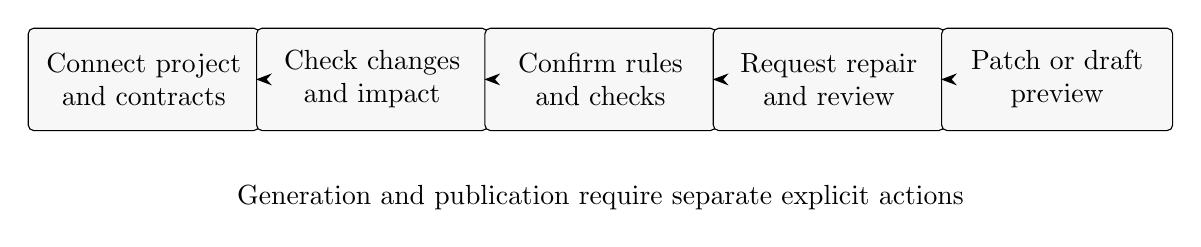
\begin{tikzpicture}
\node[reportbox] (n0) at (0.0,0) {Connect project\\and contracts};
\node[reportbox] (n1) at (2.9,0) {Check changes\\and impact};
\draw[reportarrow] (n0) -- (n1);
\node[reportbox] (n2) at (5.8,0) {Confirm rules\\and checks};
\draw[reportarrow] (n1) -- (n2);
\node[reportbox] (n3) at (8.7,0) {Request repair\\and review};
\draw[reportarrow] (n2) -- (n3);
\node[reportbox] (n4) at (11.6,0) {Patch or draft\\preview};
\draw[reportarrow] (n3) -- (n4);
\node[align=center,font=\normalsize] at (5.8,-1.5) {Generation and publication require separate explicit actions};
\end{tikzpicture}
\caption{User decisions from contract change to reviewed proposal}\label{fig:3.1}
\end{figure}

Figure~\ref{fig:3.1} identifies the decision points that prevent an observed API change from being confused with an accepted deployment. Automated comparison and test execution support those decisions, while confirmation, paid generation and remote publication remain visible actions. The workflow also permits stopping after an impact report when the available information is insufficient for repair.


% Captured application interface; original PNG retained unchanged.
The workspace overview in Figure~\ref{fig:ui-overview} brings together the selected project, API actions and recent activity.

\begin{figure}[htbp]
\centering
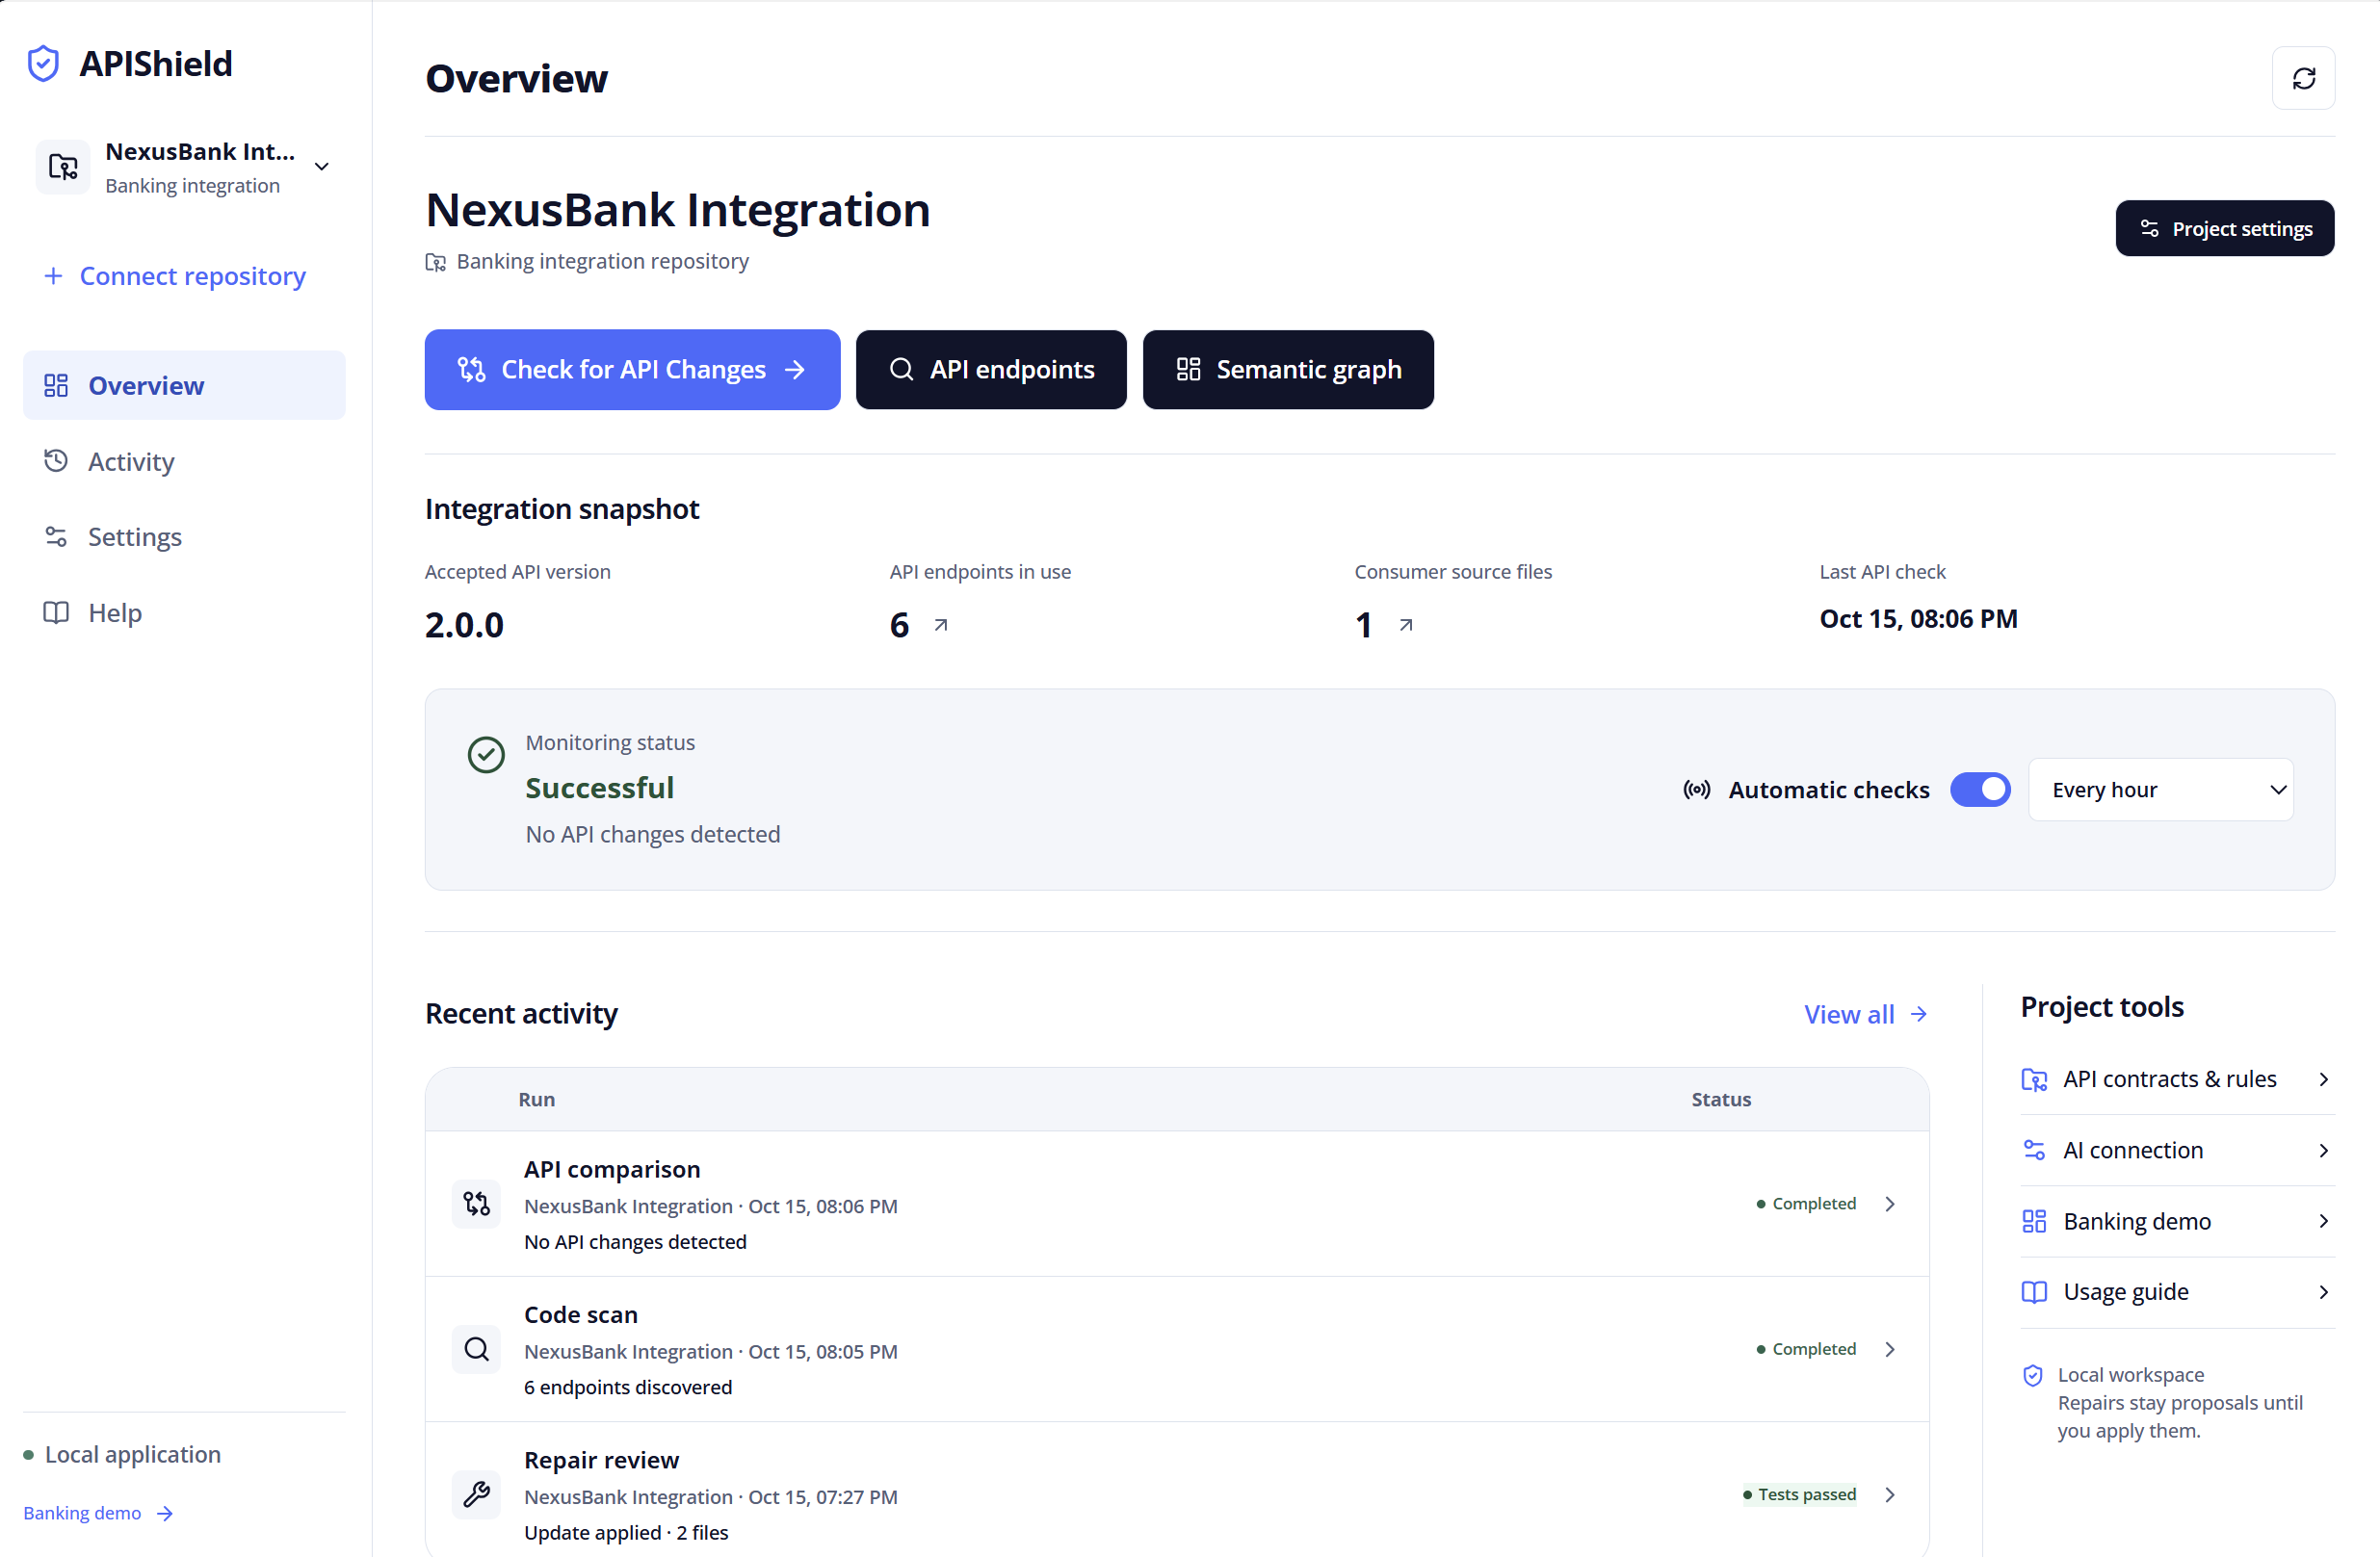
\includegraphics[width=\linewidth,height=0.65\textheight,keepaspectratio]{assets/screenshots/01_workspace_overview.png}
\caption{NexusBank workspace overview with project navigation, integration status and recent activity.}
\label{fig:ui-overview}
\end{figure}
\FloatBarrier

\section{Functional requirements}

Functional requirements were derived from the migration task and the failure cases in the original demonstration. The common engine is important because the browser and CLI must apply the same acceptance rules. A frontend status label should reflect retained engine evidence rather than infer success from a log message.

\begingroup\normalsize\onehalfspacing\setlength{\tabcolsep}{4pt}\renewcommand{\arraystretch}{1.2}
\begin{longtable}{@{}>{\raggedright\arraybackslash}p{\dimexpr 0.270\linewidth-1.080\tabcolsep\relax}>{\raggedright\arraybackslash}p{\dimexpr 0.380\linewidth-1.520\tabcolsep\relax}>{\raggedright\arraybackslash}p{\dimexpr 0.350\linewidth-1.400\tabcolsep\relax}@{}}
\caption{Functional requirements and implementation locations}\label{tab:3.1}\\
\toprule
\textbf{ID} & \textbf{Required behavior} & \textbf{Principal implementation}\\\midrule
\endfirsthead
\multicolumn{3}{l}{\small Table 3.1 continued}\\\toprule
\textbf{ID} & \textbf{Required behavior} & \textbf{Principal implementation}\\\midrule
\endhead
\bottomrule\endfoot
FR01 & Capture committed or working source & configuration.py and workspace.py\\
FR02 & Report supported calls and limitations & analysis.py\\
FR03 & Compare retained API contracts & comparison.py and native oasdiff\\
FR04 & Confirm scoped behavioral requirements & requirements.py and browser\_setup.py\\
FR05 & Validate constrained candidates & editing.py and engine.py\\
FR06 & Retain reports and cancellation state & jobs.py and dashboard\_jobs.py\\
FR07 & Monitor approved contract sources & monitoring.py and monitor\_state.py\\
FR08 & Prepare and explicitly publish full drafts & publication modules and github\_cli.py\\
FR09 & Present evidence and patch downloads & Workspace and RunEvidence components\\
\end{longtable}\endgroup

Each requirement has a boundary. For example, FR02 does not imply complete Python analysis, and FR07 does not imply operation while the local server is stopped. FR08 requires a validated retained repair and a compatible remote base; it is not a route for publishing arbitrary working-tree changes.

The traceability table supports development; it does not independently certify the implementation. The implementation and regression tests supply the actual behavior, while dated validation records show selected executions, including the banking fixture (APIShield Project, 2026a). Future changes should update the affected requirement row and evidence references together so that a renamed module does not leave the report describing an obsolete interface.

\section{Quality requirements and execution limits}

Correctness evidence, recoverability and source preservation are more important than unrestricted autonomy in the initial product. A failed candidate must not leave an edited original repository, and an unavailable model must not produce a fabricated validated status. A timed-out or cancelled command must retain its outcome even if partial output appears successful.

The engine uses finite budgets for attempts, command duration, total job duration and captured output. The defaults are configuration values, not measured performance claims. Specific acceptance runs use their own recorded limits, which are reported with those cohorts.

\begingroup\normalsize\onehalfspacing\setlength{\tabcolsep}{4pt}\renewcommand{\arraystretch}{1.2}
\begin{longtable}{@{}>{\raggedright\arraybackslash}p{\dimexpr 0.270\linewidth-1.080\tabcolsep\relax}>{\raggedright\arraybackslash}p{\dimexpr 0.380\linewidth-1.520\tabcolsep\relax}>{\raggedright\arraybackslash}p{\dimexpr 0.350\linewidth-1.400\tabcolsep\relax}@{}}
\caption{Default local execution budgets}\label{tab:3.2}\\
\toprule
\textbf{Setting} & \textbf{Default} & \textbf{Interpretation}\\\midrule
\endfirsthead
\multicolumn{3}{l}{\small Table 3.2 continued}\\\toprule
\textbf{Setting} & \textbf{Default} & \textbf{Interpretation}\\\midrule
\endhead
\bottomrule\endfoot
Repair attempts & 3 & Maximum engine attempts for live generation\\
Command timeout & 120 seconds & Upper limit for one repository command\\
Job timeout & 600 seconds & Overall execution deadline\\
Captured output & 65,536 bytes & Bound on recorded command output\\
Browser worker pool & 2 workers & Local background job executor size\\
\end{longtable}\endgroup

Recoverability includes durable results, interrupted-worker detection, process-tree cleanup and explicit publication reconciliation. Local filesystem records are appropriate for a single-machine prototype, but they do not provide the availability or isolation guarantees of a hosted service.

Usability requires that evidence remain accessible without opening every raw artifact. The interface therefore separates overview, impact, proposed changes, tests and technical provenance. Accessibility includes keyboard navigation and a graph List fallback. Eight current application captures document the interface views illustrated in this report. Screenshot inspection establishes their displayed appearance; keyboard navigation, drag behavior and responsive interactions require separate acceptance checks.

\section{Behavioral requirements and acceptance obligations}

A behavioral requirement identifies a property that a migration should preserve. The current declaration includes an identifier, prose description, exact file/function scope, origin, confirmation status and selected pytest references. Its canonical hash becomes part of the run record, allowing a reviewer to distinguish a current rule from the rule captured by an earlier job.

For shipping, a representative rule preserves package identity and exact integer gram weight. For payment, a useful obligation preserves the exact cents value supplied by the caller. Refund behavior additionally requires the correct operation and transaction identity. An invoice migration may need information absent from the function inputs; in that case a diagnostic is the admissible outcome.

\begingroup\normalsize\onehalfspacing\setlength{\tabcolsep}{4pt}\renewcommand{\arraystretch}{1.2}
\begin{longtable}{@{}>{\raggedright\arraybackslash}p{\dimexpr 0.270\linewidth-1.080\tabcolsep\relax}>{\raggedright\arraybackslash}p{\dimexpr 0.380\linewidth-1.520\tabcolsep\relax}>{\raggedright\arraybackslash}p{\dimexpr 0.350\linewidth-1.400\tabcolsep\relax}@{}}
\caption{Example preservation rules and independent observations}\label{tab:3.3}\\
\toprule
\textbf{Rule} & \textbf{Observable obligation} & \textbf{Failure example}\\\midrule
\endfirsthead
\multicolumn{3}{l}{\small Table 3.3 continued}\\\toprule
\textbf{Rule} & \textbf{Observable obligation} & \textbf{Failure example}\\\midrule
\endhead
\bottomrule\endfoot
Exact amount & Integer payload equals caller amount & Float conversion loses a large integer\\
Identity & Identifier survives the request unchanged & Customer or package ID replaced\\
Operation & Request uses the intended action & Refund changed into charge\\
Response behavior & Returned value follows actual provider reply & Hardcoded success ignores transport\\
Missing information & No unsupported data invented & Default address silently inserted\\
\end{longtable}\endgroup

Confirmation means that a developer approved the definition and its current scope. It does not prove the prose or guarantee that the linked tests are complete. Editing the definition or changing repository/source/test context clears confirmation. During repair, applicable confirmed rules with unresolved scope or unavailable checks require input. The engine records discovery and execution evidence separately so that a syntactically valid test reference cannot masquerade as an executed passing assertion (APIShield Project, 2026d).

\section{Constraints, assumptions and feasibility}

The implementation assumes trusted repositories because setup and tests execute code on the local host. Candidate isolation protects source preservation, while host security remains the operator's responsibility. No customer account system or tenant boundary is present. The launcher binds the application to loopback, consistent with that operating model.

Native oasdiff, Git, Python and frontend build tooling are prerequisites. The model connection is optional for offline examples. Live generation uses a selected Gemini connection; service-account credentials captured through the browser remain in server memory. GitHub drafts use the existing local GitHub CLI credential store. These integrations have distinct lifetimes and failure modes.

Technical feasibility is supported by the implemented shipping and banking examples and the recorded live acceptance cases. Research feasibility is supported by an opt-in harness, retained patches and independent checks. Neither establishes that a large real-world study will have a positive result. Environment preparation, fixture selection and oracle quality can dominate effort when moving beyond synthetic examples.

The project excludes automatically merging or deploying changes. That decision keeps publication evidence separate from application release. It also makes the product usable when a model fails: the developer can still inspect contract differences and source impact without requesting generation.

Supported coverage could be extended through deeper field observations, broader call resolution and per-integration test environments. Controlled baselines can test the proposed academic contribution. Hosted scheduling and isolated workers require a separate architecture. These are different deliverables and should not be presented as if completion of one automatically establishes the others.

\chapter{SYSTEM ARCHITECTURE AND DATA DESIGN}
\section{Architecture overview}

APIShield has a browser presentation layer, a FastAPI coordination layer and a reusable Python execution engine. The browser submits an integration operation and reads retained evidence. The API validates requests, coordinates local background work and exposes job, monitoring, model and publication endpoints. The engine performs the captured-source repair transaction.

The command-line interface calls the same engine. This reduces the risk that a browser shortcut bypasses the acceptance checks described in the methodology. A deterministic offline candidate uses the same editing and validation stages as model output, while bypassing inference.

\begin{figure}[htbp]\centering
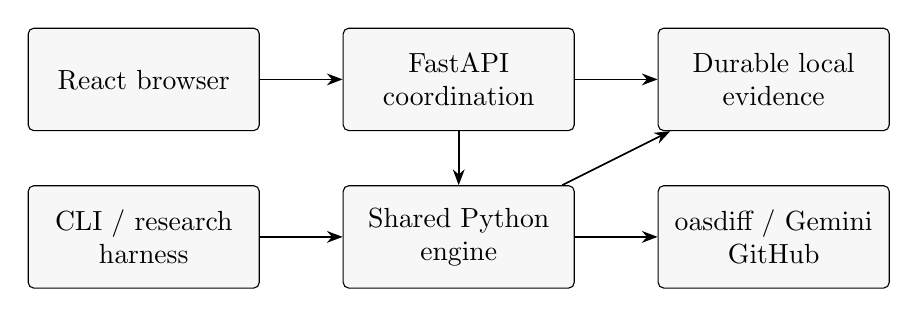
\begin{tikzpicture}
\node[reportbox] (browser) at (0,2) {React browser};
\node[reportbox] (cli) at (0,0) {CLI / research\\harness};
\node[reportbox] (api) at (4,2) {FastAPI\\coordination};
\node[reportbox] (engine) at (4,0) {Shared Python\\engine};
\node[reportbox] (records) at (8,2) {Durable local\\evidence};
\node[reportbox] (external) at (8,0) {oasdiff / Gemini\\GitHub};
\draw[reportarrow] (browser) -- (api);
\draw[reportarrow] (cli) -- (engine);
\draw[reportarrow] (api) -- (engine);
\draw[reportarrow] (api) -- (records);
\draw[reportarrow] (engine) -- (external);
\draw[reportarrow] (engine) -- (records);
\end{tikzpicture}
\caption{Current local architecture and external boundaries}\label{fig:4.1}
\end{figure}

The local job store persists configuration snapshots, contract copies, events, command evidence and results. Temporary workspaces are removed when jobs finish, while validated patches remain available. Monitoring and publication maintain their own durable lifecycle records under the local storage root.

External boundaries are explicit: native oasdiff supplies comparison evidence; a configured Gemini endpoint supplies candidate generation or optional graph interpretation; GitHub CLI mediates publication. The provider and SwiftPay services belong to the legacy demonstration and can run separately. A normal shipping-example workflow does not need those payment services or a model connection.

Figure~\ref{fig:4.1} shows the current local deployment. The roadmap also includes a database-backed queue, container workers and a tenant-aware service; these remain future work.

\section{Backend modules and responsibilities}

The apishield package separates configuration, source preparation, analysis, execution and publication. Its boundaries are logical responsibilities rather than independently deployed services. Keeping the engine free of browser state allows both interfaces and the research harness to invoke the same core operation.

\begingroup\normalsize\onehalfspacing\setlength{\tabcolsep}{4pt}\renewcommand{\arraystretch}{1.2}
\begin{longtable}{@{}>{\raggedright\arraybackslash}p{\dimexpr 0.270\linewidth-1.080\tabcolsep\relax}>{\raggedright\arraybackslash}p{\dimexpr 0.380\linewidth-1.520\tabcolsep\relax}>{\raggedright\arraybackslash}p{\dimexpr 0.350\linewidth-1.400\tabcolsep\relax}@{}}
\caption{Backend subsystem responsibilities}\label{tab:4.1}\\
\toprule
\textbf{Subsystem} & \textbf{Principal files} & \textbf{Responsibility}\\\midrule
\endfirsthead
\multicolumn{3}{l}{\small Table 4.1 continued}\\\toprule
\textbf{Subsystem} & \textbf{Principal files} & \textbf{Responsibility}\\\midrule
\endhead
\bottomrule\endfoot
Configuration & configuration.py & Validate paths, commands, budgets and rules\\
Source snapshot & workspace.py & Read pinned Git objects into a disposable copy\\
Analysis & analysis.py and repository\_graph.py & Observe supported calls and source relationships\\
Execution & engine.py and commands.py & Bound attempts, run commands and enforce acceptance\\
Evidence & jobs.py and overview.py & Persist records and reconstruct retained views\\
Model access & generation.py and model\_access.py & Select connection and request structured output\\
Monitoring & monitoring.py and contract\_fetch.py & Fetch approved contracts and reserve comparison work\\
Publication & publication.py and publication\_prepare.py & Revalidate complete patch and coordinate drafts\\
\end{longtable}\endgroup

dashboard\_api.py still includes payment-demo control state. The newer browser routes are attached through dedicated modules, including browser\_setup.py, dashboard\_jobs.py and publication\_api.py. This coexistence explains why the repository contains both an older mutable repair demonstration and a newer isolated workflow.

A fix to the legacy agent does not automatically change the shared engine. Claims about source-preserving jobs therefore refer to the isolated execution path. The retained examples and regression tests help prevent the two execution models from being confused.

\section{Job lifecycle and durable records}

A job has an identity, operation, configuration snapshot and filesystem location. Its source revision and contract hashes establish the inputs. Scan and comparison jobs can complete without proposing edits; repair jobs add candidate attempts and validation evidence. Terminal outcomes distinguish validated, failed, cancelled, no change and needs input.

\begin{figure}[htbp]\centering
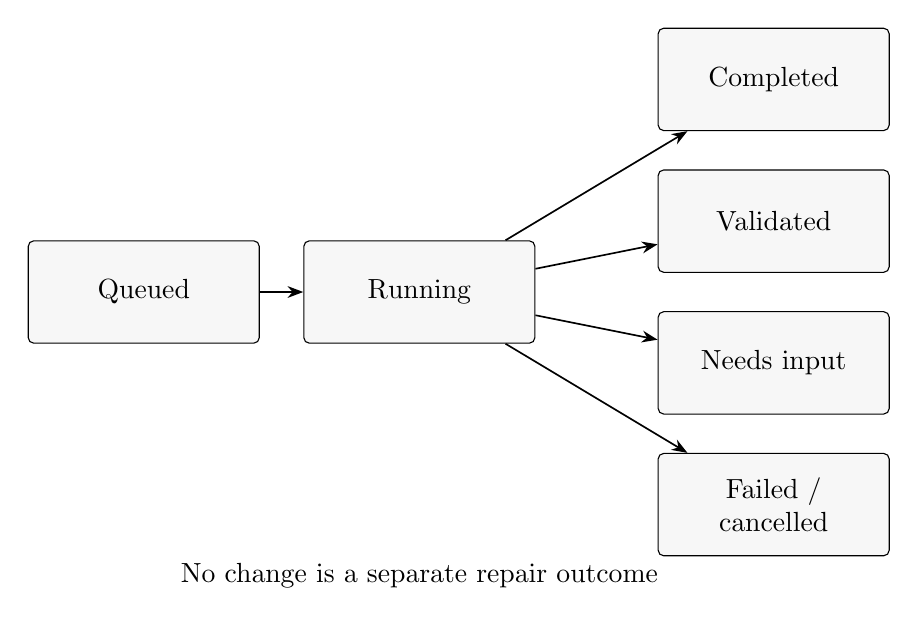
\begin{tikzpicture}
\node[reportbox] (queued) at (0,0) {Queued};
\node[reportbox] (running) at (3.5,0) {Running};
\node[reportbox] (completed) at (8,2.7) {Completed};
\node[reportbox] (validated) at (8,0.9) {Validated};
\node[reportbox] (input) at (8,-0.9) {Needs input};
\node[reportbox] (failed) at (8,-2.7) {Failed / cancelled};
\draw[reportarrow] (queued) -- (running);
\draw[reportarrow] (running) -- (completed);
\draw[reportarrow] (running) -- (validated);
\draw[reportarrow] (running) -- (input);
\draw[reportarrow] (running) -- (failed);
\node[align=center,font=\normalsize] at (3.5,-3.6) {No change is a separate repair outcome};
\end{tikzpicture}
\caption{Job lifecycle with guarded acceptance outcomes}\label{fig:4.2}
\end{figure}

OS-level ownership locks prevent two local workers from executing the same retained job concurrently. The store uses atomic replacement for structured records. Cancellation is persisted and checked during work; an interrupted process is detected rather than silently resumed from a partially applied candidate.

The worker captures source metadata before analysis and retains it independently of the disposable workspace. Each attempt records setup and validation commands, errors and requirement outcomes. A validated patch is written from the engine's independently checked candidate bytes. Failed jobs do not offer a patch as if it had passed.

Recovery does not mean that every operation can be undone. Local workspace cleanup is different from a remote GitHub request whose response was lost. The publication subsystem therefore has reconciliation states in addition to ordinary execution failure. This keeps a valid local repair from being relabeled invalid merely because publication encountered an uncertain remote effect.

The filesystem store is intentionally local. Its lock and atomic-write mechanisms support the current usage, but a distributed worker pool would need different coordination and recovery design. The existence of durable JSON records should not be described as a complete distributed job platform.

\section{Source, contract and requirement records}

Committed-mode records identify the pinned commit and excluded working edits; the engine reads raw Git blobs. Working-mode records retain file hashes and captured bytes so current browser operations include uncommitted source. Both modes bind validation to a stable captured input. Symlink or submodule entries are unsupported; known secret-file patterns are excluded from exported content.

Contract snapshots and their hashes retain the versions used for the original decision. Comparison and revalidation use those versions even if the current files have changed. The run also captures the complete selected requirement set and its canonical hash.

\begingroup\normalsize\onehalfspacing\setlength{\tabcolsep}{4pt}\renewcommand{\arraystretch}{1.2}
\begin{longtable}{@{}>{\raggedright\arraybackslash}p{\dimexpr 0.270\linewidth-1.080\tabcolsep\relax}>{\raggedright\arraybackslash}p{\dimexpr 0.380\linewidth-1.520\tabcolsep\relax}>{\raggedright\arraybackslash}p{\dimexpr 0.350\linewidth-1.400\tabcolsep\relax}@{}}
\caption{Retained records and their provenance role}\label{tab:4.2}\\
\toprule
\textbf{Record} & \textbf{Representative contents} & \textbf{Purpose}\\\midrule
\endfirsthead
\multicolumn{3}{l}{\small Table 4.2 continued}\\\toprule
\textbf{Record} & \textbf{Representative contents} & \textbf{Purpose}\\\midrule
\endhead
\bottomrule\endfoot
Configuration & Repository, ref, paths, commands and budgets & Reconstruct selected execution inputs\\
Source metadata & Source mode, commit and captured file hashes & Identify the exact analyzed source\\
Contracts & Original and updated JSON plus hashes & Bind comparison to exact descriptions\\
Requirement set & Definitions, checks and canonical hash & Bind acceptance to reviewed declarations\\
Attempts & Commands, outputs and requirement results & Explain candidate acceptance or rejection\\
Final result & Status, errors and patch digest & Expose durable review outcome\\
\end{longtable}\endgroup

Hashing detects selected evidence changes when the relevant checks are performed. It is not a digital signature or an assurance against every actor with local filesystem access. Provenance depends on retaining exact inputs and checking their consistency at transitions such as publication preparation.

Later edits to an integration create new configuration context. They do not rewrite previous job evidence. Historical overview enrichment reads retained snapshots with guards, preserving the distinction between the original run and a current presentation of its data.


% Captured application interface; original PNG retained unchanged.
Figure~\ref{fig:ui-project-settings} shows how the local repository and its validation command are presented in project settings.

\begin{figure}[htbp]
\centering
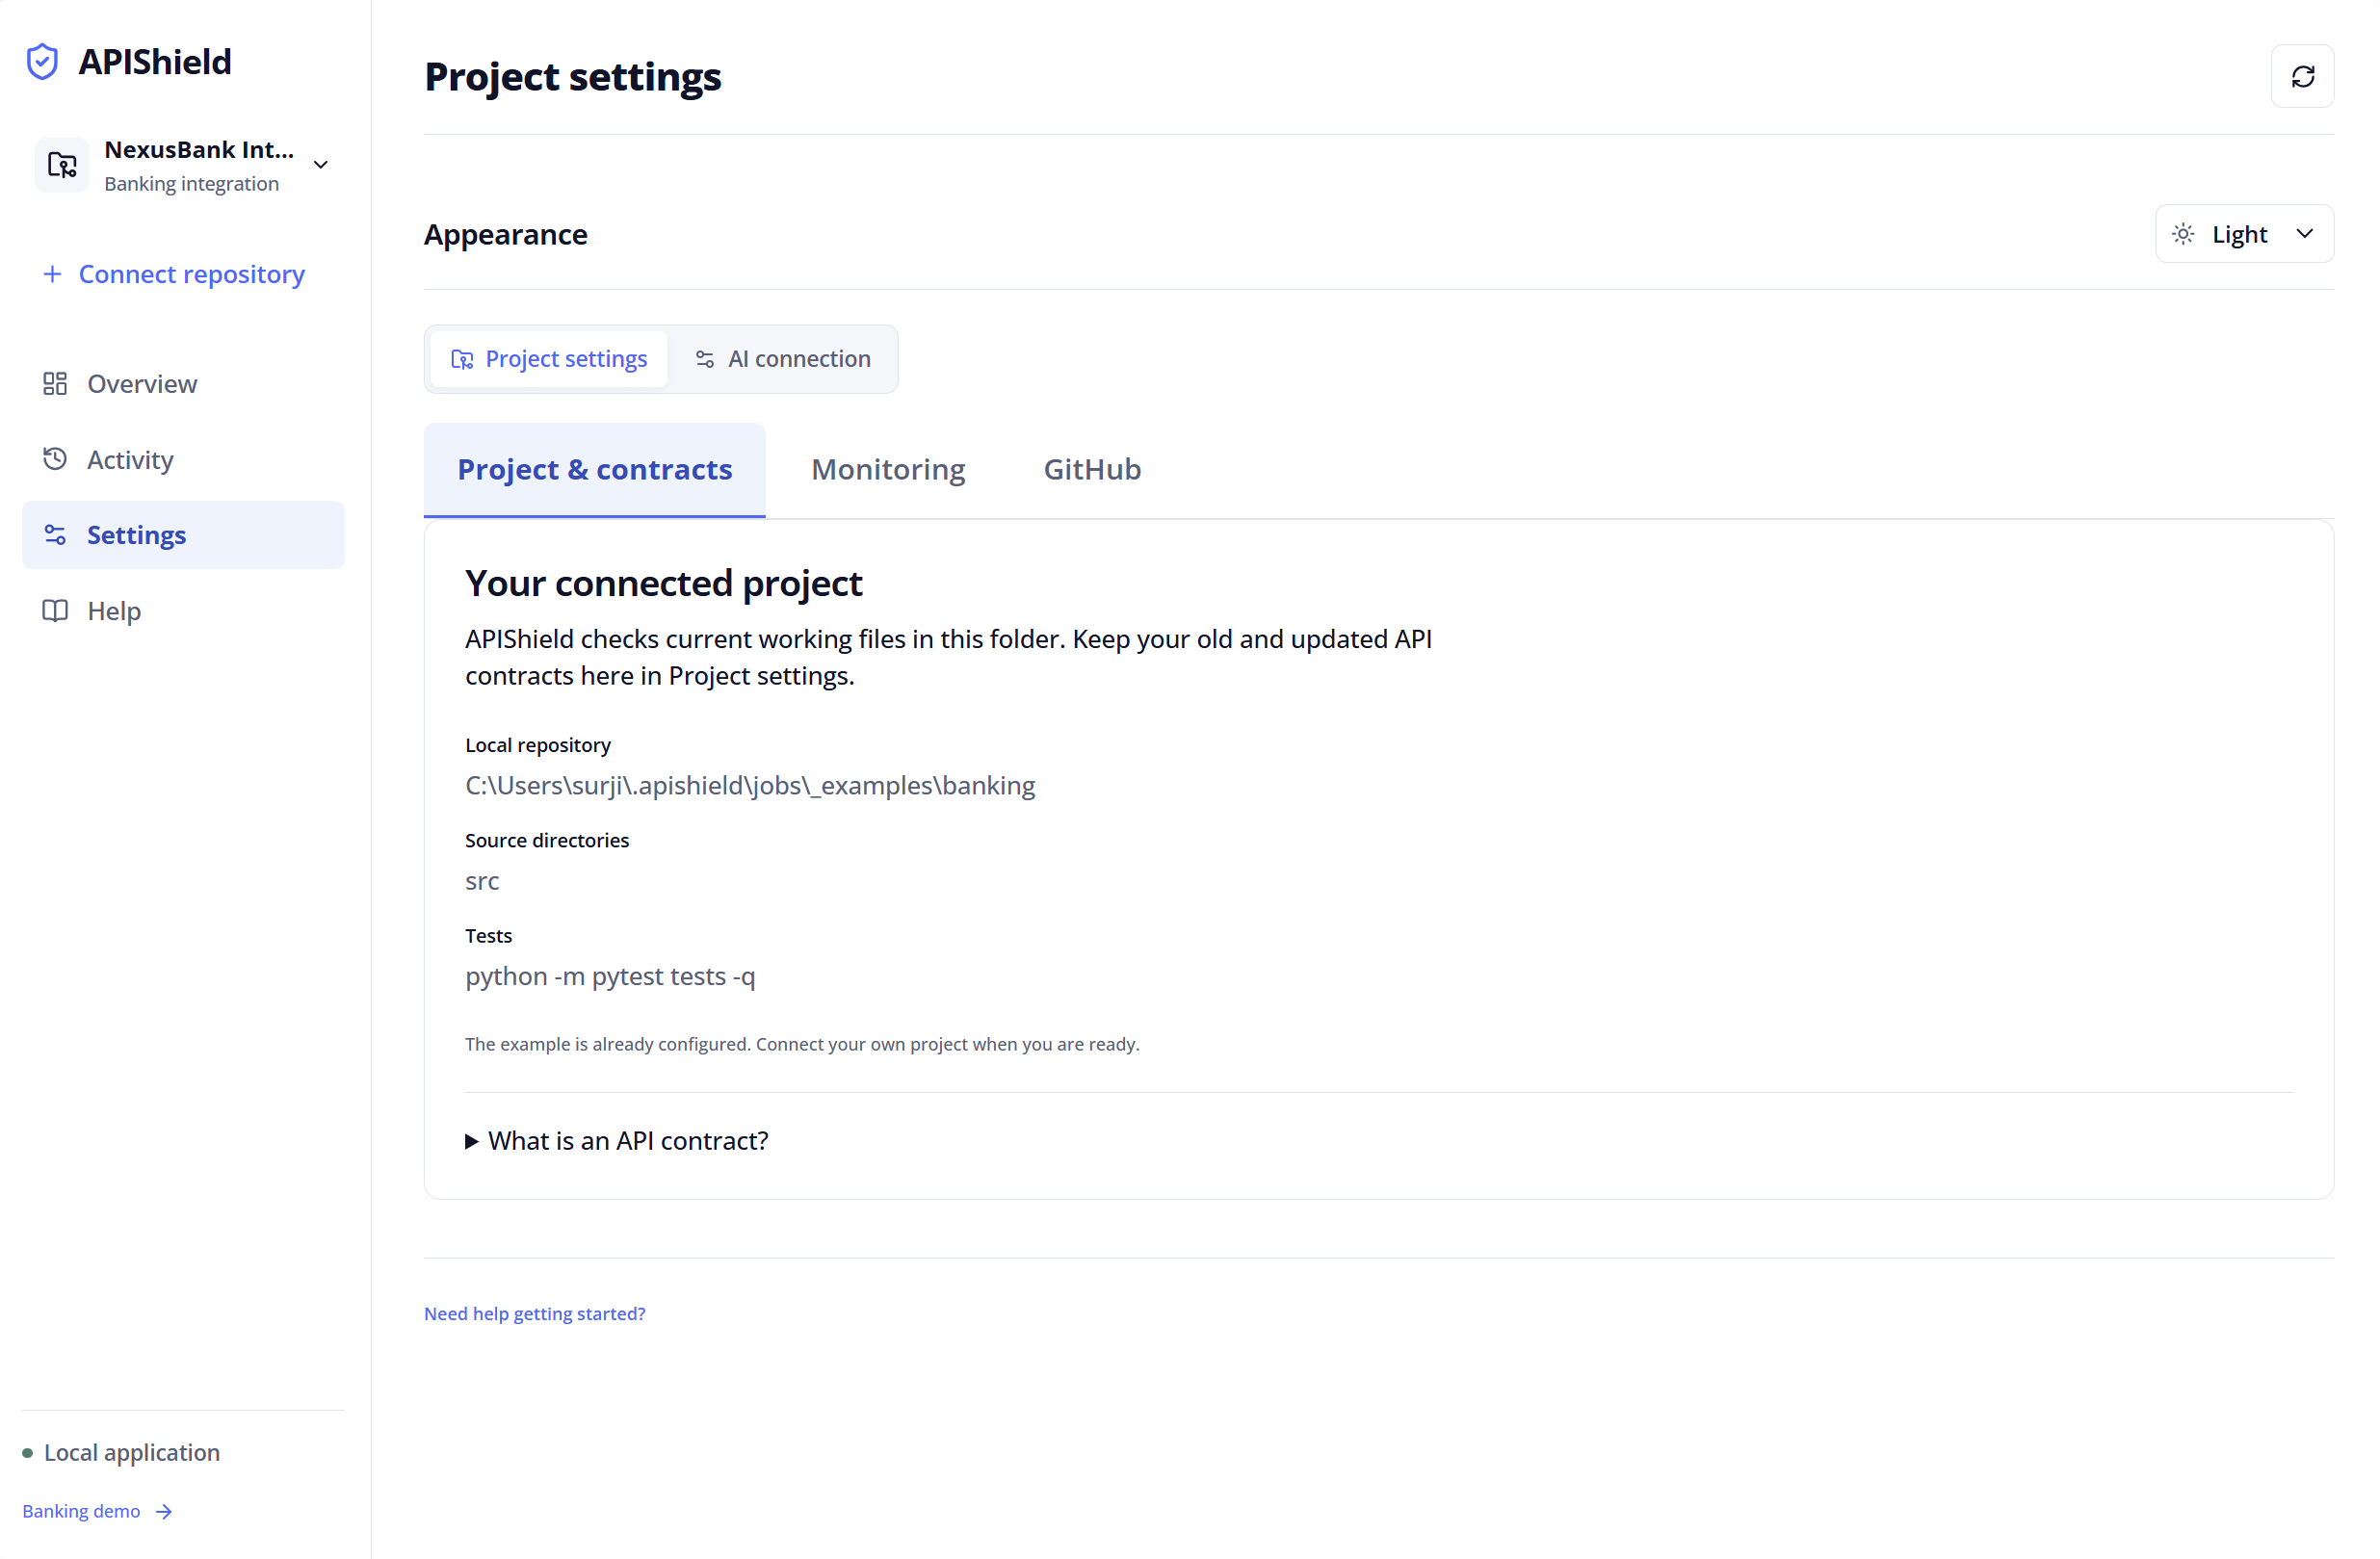
\includegraphics[trim=290bp 0 0 0,clip,width=\linewidth,height=0.65\textheight,keepaspectratio]{assets/screenshots/02_project_contracts.png}
\caption{Project settings showing the connected example repository, source directory and configured test command.}
\label{fig:ui-project-settings}
\end{figure}
\FloatBarrier

\section{Repository graph and evidence provenance}

The repository graph includes supported files, classes, functions, tests and API operations. Python AST traversal supplies declarations and selected call relationships. Source docstrings can supply declared intents. Developer requirements link function scopes to selected tests. Limited JavaScript and TypeScript analysis adds named functions and literal fetch-route relationships.

\begin{figure}[htbp]\centering
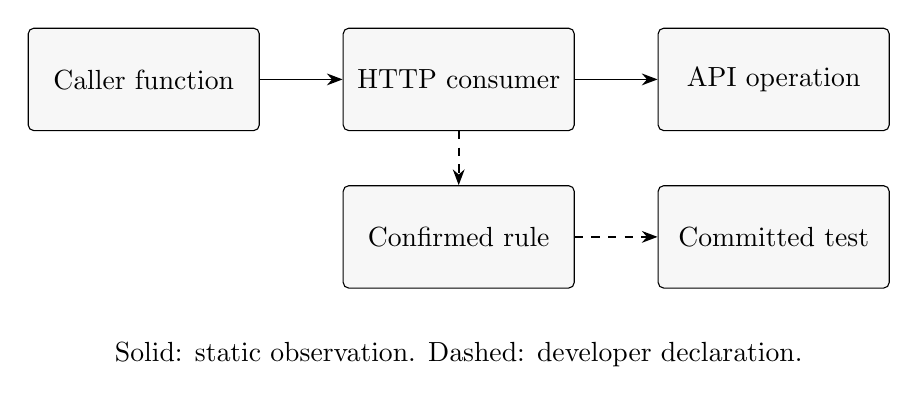
\begin{tikzpicture}
\node[reportbox] (caller) at (0,2) {Caller function};
\node[reportbox] (consumer) at (4,2) {HTTP consumer};
\node[reportbox] (operation) at (8,2) {API operation};
\node[reportbox] (rule) at (4,0) {Confirmed rule};
\node[reportbox] (test) at (8,0) {Committed test};
\draw[reportarrow] (caller) -- (consumer);
\draw[reportarrow] (consumer) -- (operation);
\draw[reportarrow,dashed] (consumer) -- (rule);
\draw[reportarrow,dashed] (rule) -- (test);
\node[align=center,font=\normalsize] at (4,-1.5) {Solid: static observation. Dashed: developer declaration.};
\end{tikzpicture}
\caption{Observed and declared relationships in a migration graph}\label{fig:4.3}
\end{figure}

An operation changed by contract comparison and its direct consuming function receive direct impact. Resolved callers can receive potential impact. Potential impact means dependence on affected code, not an observed runtime failure. The node inspector records that reason so that a red mark does not imply more evidence than exists.

The graph scan is bounded to 500 files, 256 KiB per file and 2 MiB of source text. Its own coverage notes accompany the graph. Dynamic dispatch, ambiguous routes and unsupported syntax remain unresolved. The graph's broader structural coverage does not expand the set of files the repair engine may edit.

Community detection groups recorded relationships for presentation. Optional Gemini interpretation can assign business-flow communities and separately labeled inferred links. Those overlays are tied to the graph hash and validated against existing node identities. They do not add verified calls, alter impact localization or satisfy requirements. This boundary permits an interpretive display without treating a model's explanation as executable evidence (APIShield Project, 2026c).


% Captured application interface; original PNG retained unchanged.
The captured structural view in Figure~\ref{fig:ui-impact-graph} groups code and API relationships. Its displayed state has no detected impact; affected-call localization is illustrated separately in Figure~\ref{fig:ui-change-detection}.

\begin{figure}[htbp]
\centering
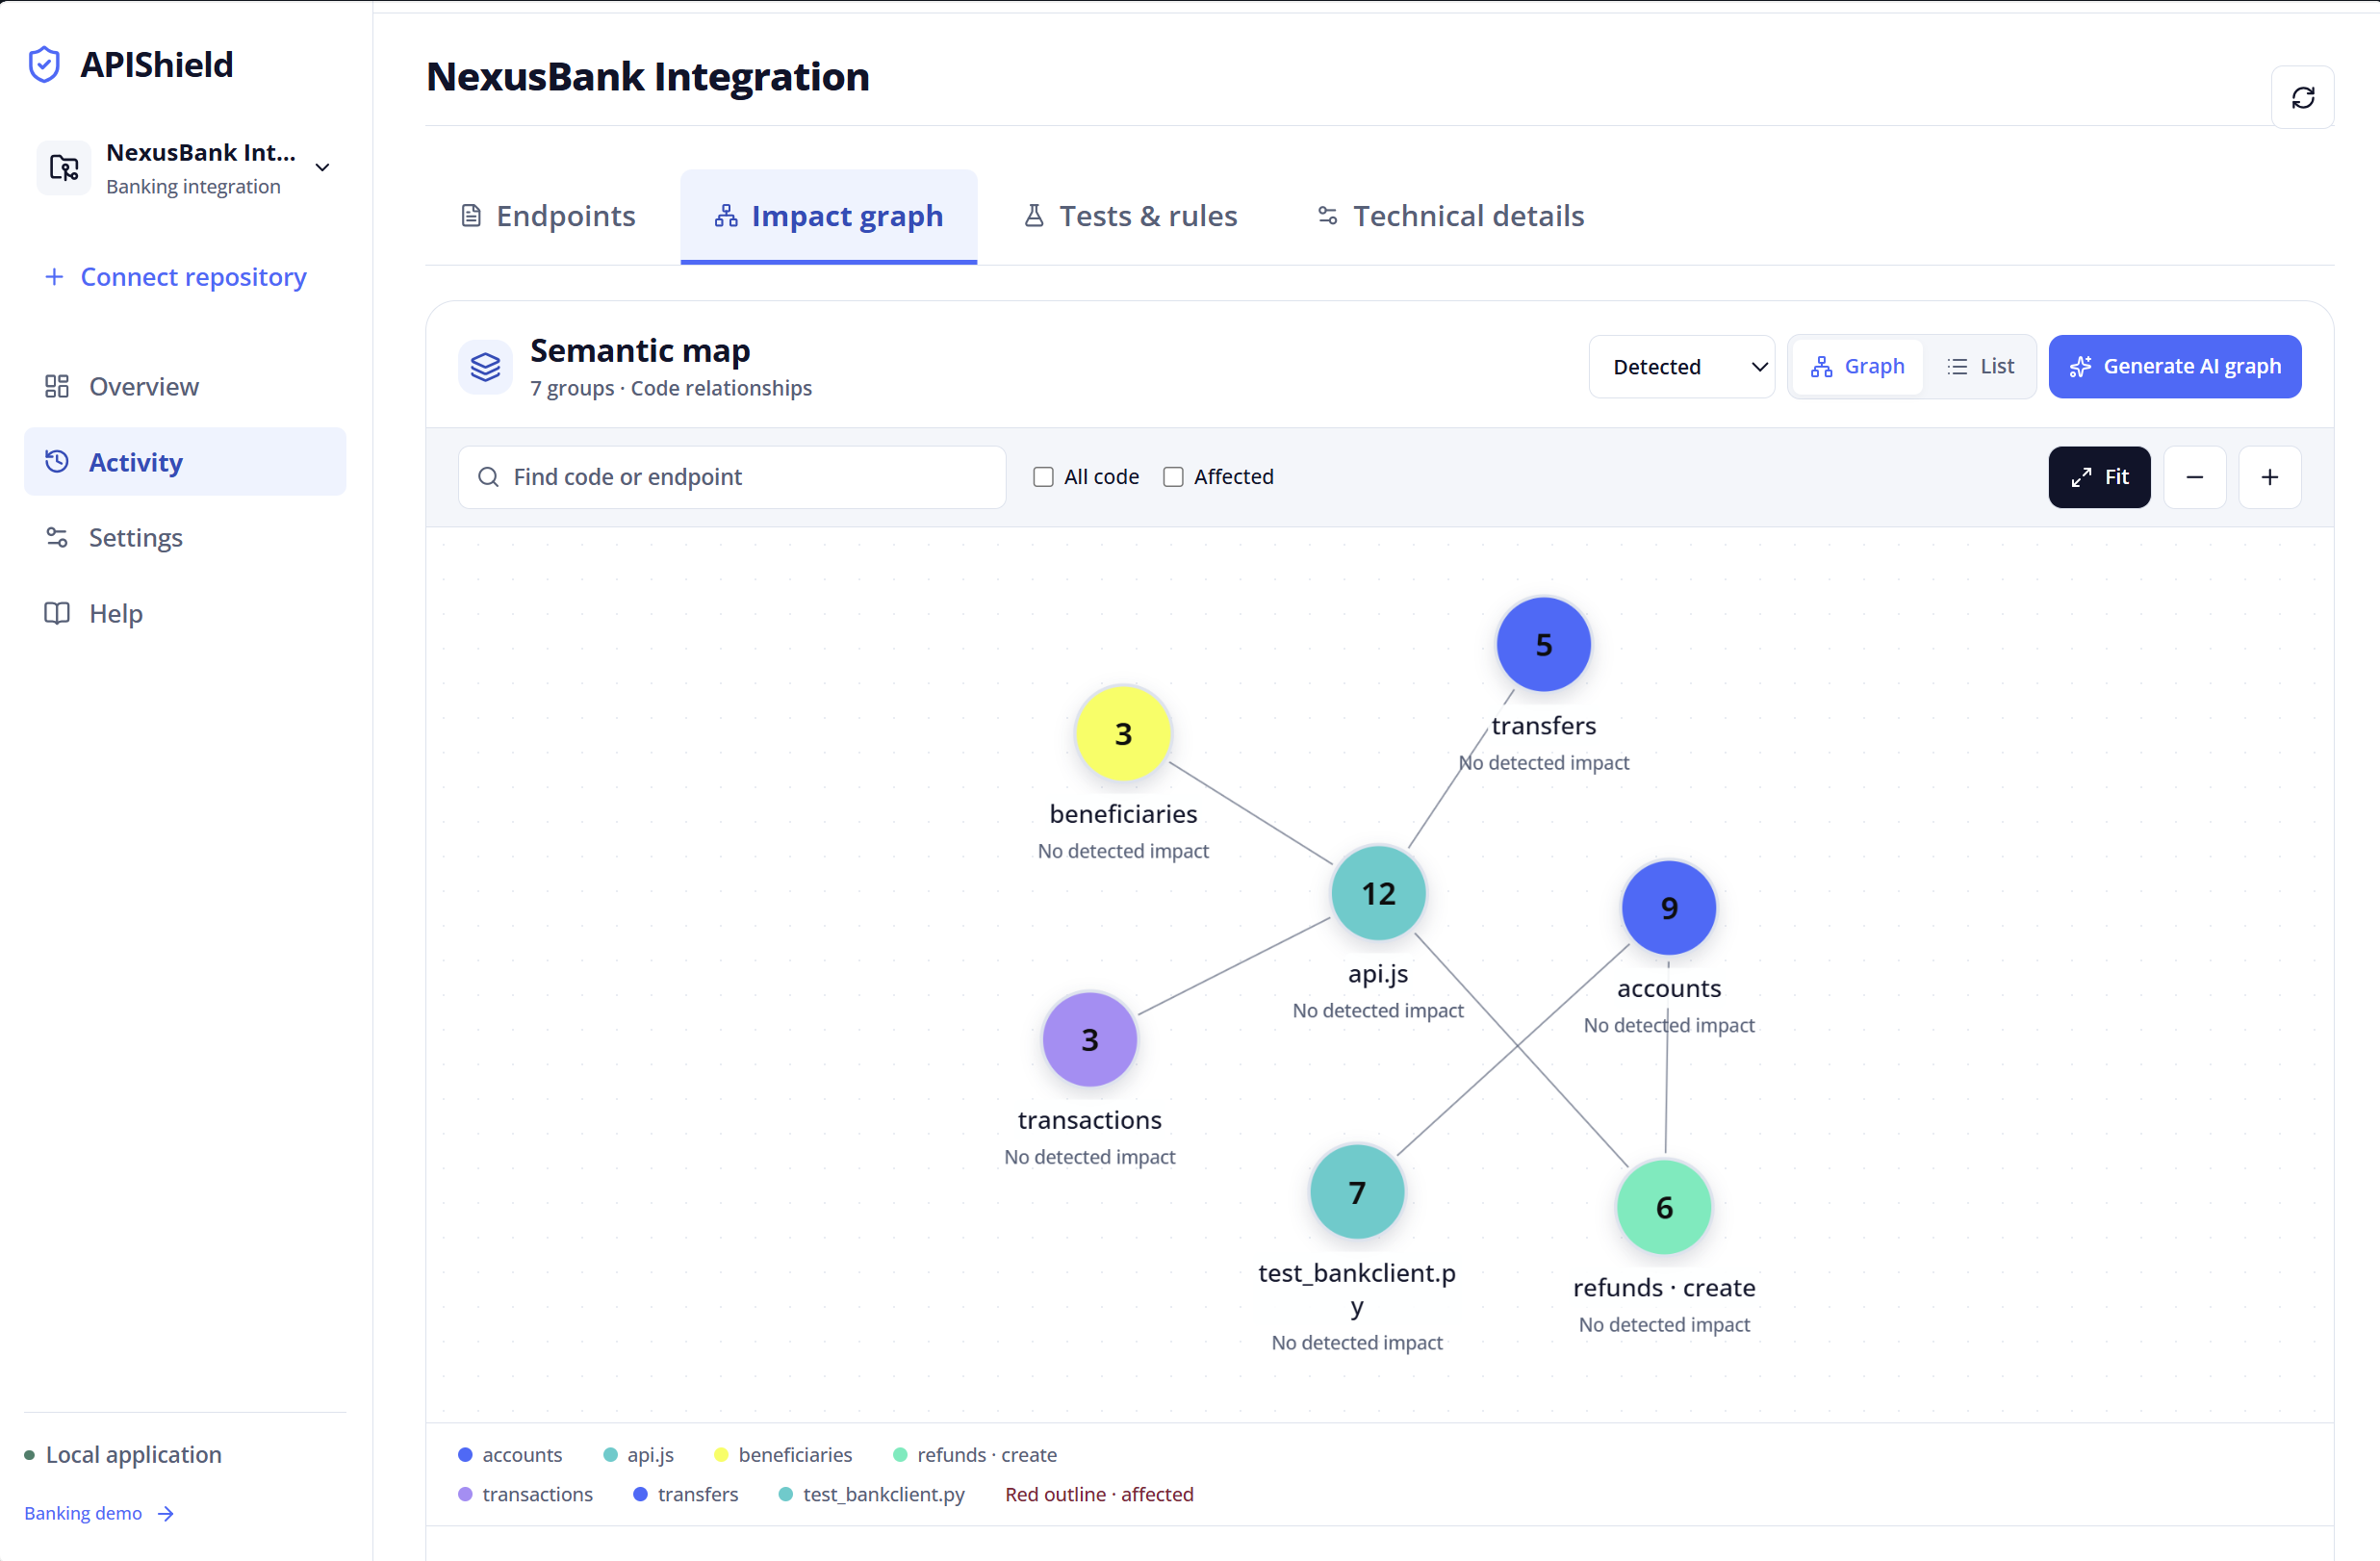
\includegraphics[trim=290bp 0 0 0,clip,width=\linewidth,height=0.65\textheight,keepaspectratio]{assets/screenshots/03_impact_graph.png}
\caption{Detected structural groups in the NexusBank impact graph; the displayed snapshot reports no detected impact.}
\label{fig:ui-impact-graph}
\end{figure}
\FloatBarrier

\section{Browser review workspace}

The React workspace exposes current API views, retained runs, code changes, tests, settings and optional GitHub drafts through structured engine reports.

Current views show active contracts and consumers; change reports retain paired contracts and impact evidence. The graph supports source inspection and a List fallback. Reviewed Apply writes repairs and generated tests without a commit, rejects stale inputs and retains recovery bytes. Success accepts the captured contract and refreshes the current graph while preserving historical evidence (APIShield Project, 2026j).

\begingroup\normalsize\onehalfspacing\setlength{\tabcolsep}{4pt}\renewcommand{\arraystretch}{1.2}
\begin{longtable}{@{}>{\raggedright\arraybackslash}p{\dimexpr 0.270\linewidth-1.080\tabcolsep\relax}>{\raggedright\arraybackslash}p{\dimexpr 0.380\linewidth-1.520\tabcolsep\relax}>{\raggedright\arraybackslash}p{\dimexpr 0.350\linewidth-1.400\tabcolsep\relax}@{}}
\caption{Review panels and the decision each supports}\label{tab:4.3}\\
\toprule
\textbf{Panel} & \textbf{Evidence shown} & \textbf{Review question}\\\midrule
\endfirsthead
\multicolumn{3}{l}{\small Table 4.3 continued}\\\toprule
\textbf{Panel} & \textbf{Evidence shown} & \textbf{Review question}\\\midrule
\endhead
\bottomrule\endfoot
Overview & Original and updated contract details & What changed in the described interface?\\
Impact graph & Observed and declared relationships & Which supported consumers may be affected?\\
Code changes & Retained candidate patch & What exactly does the proposal edit?\\
Tests and rules & Commands and separate requirement outcomes & Which assertions were actually checked?\\
Technical details & Coverage and provenance & What revision and limitations apply?\\
GitHub draft & Prepared full proposal and state & What will be published and has it succeeded?\\
\end{longtable}\endgroup

The architecture diagrams describe system interfaces, while the accompanying application captures document the current browser views. The image review covers the displayed states; it does not establish acceptance of every interactive behavior.


% Captured application interface; original PNG retained unchanged.
Figure~\ref{fig:ui-code-changes} shows the review surface for a banking migration proposal. The visible excerpt changes the balance response lookup and transfer payload structure; the complete patch remains available for download.

\begin{figure}[htbp]
\centering
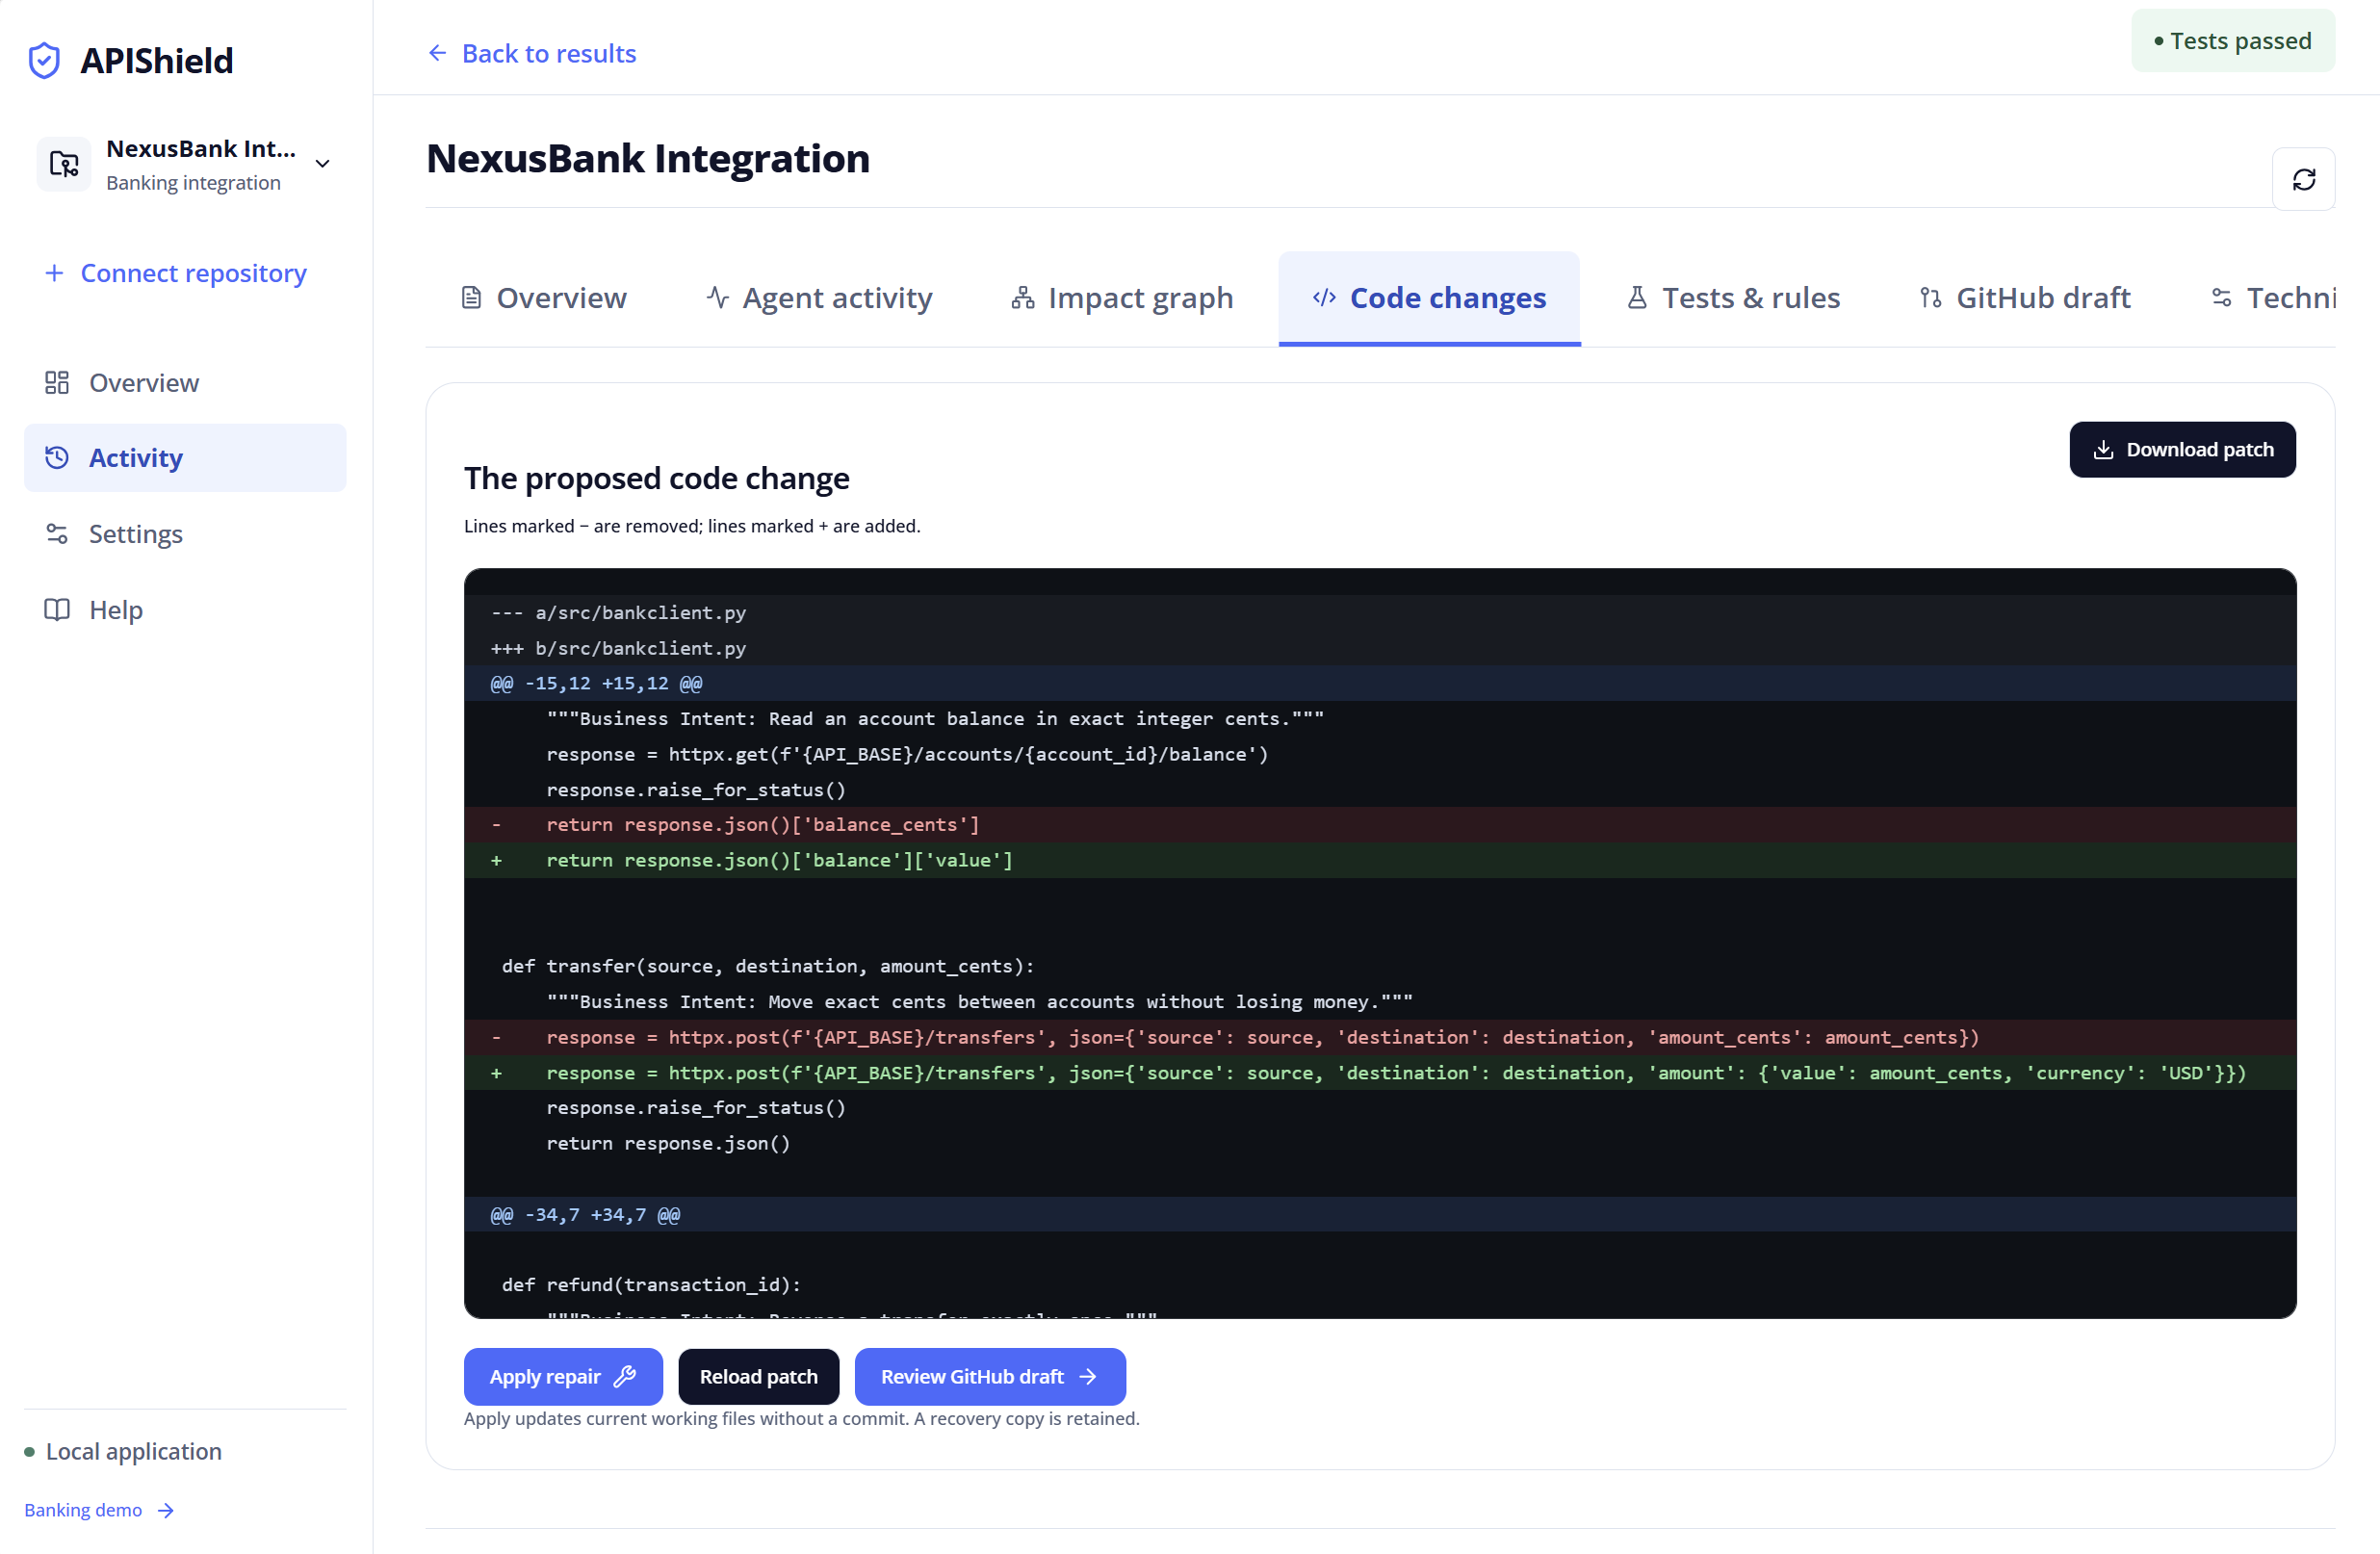
\includegraphics[trim=290bp 0 0 0,clip,width=\linewidth,height=0.65\textheight,keepaspectratio]{assets/screenshots/05_repair_code_changes.png}
\caption{Repair review showing an excerpt of the banking client patch, validation status and explicit Apply controls.}
\label{fig:ui-code-changes}
\end{figure}
\FloatBarrier

\section{Monitoring and publication coordination}

Monitoring stores an approved contract source, an interval, a baseline and immutable fetched versions. A scheduled check reserves comparison work, deduplicates a known change and exposes its report. Baseline acceptance is explicit. A rescan can update code impact for a retained change without pretending that the provider published another version (APIShield Project, 2026h).

Publication begins with a validated retained repair. Preparation reconstructs its complete patch using guarded Git patch operations and runs offline validation against the pinned source (Git project, n.d.). The preview binds repository, base, patch and evidence to revisions. Publication then checks remote state and creates a draft through the existing GitHub CLI sign-in.

\begin{figure}[htbp]\centering
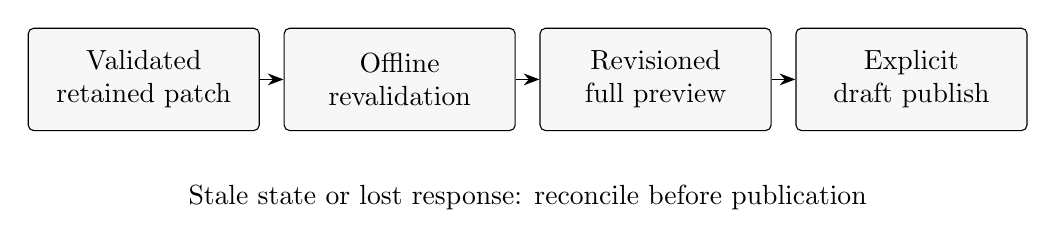
\begin{tikzpicture}
\node[reportbox] (n0) at (0.0,0) {Validated\\retained patch};
\node[reportbox] (n1) at (3.25,0) {Offline\\revalidation};
\draw[reportarrow] (n0) -- (n1);
\node[reportbox] (n2) at (6.5,0) {Revisioned\\full preview};
\draw[reportarrow] (n1) -- (n2);
\node[reportbox] (n3) at (9.75,0) {Explicit\\draft publish};
\draw[reportarrow] (n2) -- (n3);
\node[align=center,font=\normalsize] at (4.875,-1.5) {Stale state or lost response: reconcile before publication};
\end{tikzpicture}
\caption{Separate repair validation and draft publication}\label{fig:4.4}
\end{figure}

These are separate state machines because their failures differ. A provider fetch can fail without invalidating previous change evidence. A remote publish response can be lost even though a draft was created. Reconciliation checks retained identity and remote effects before another write, reducing duplicate proposals.





\chapter{METHODOLOGY AND IMPLEMENTATION}
\section{Source capture and workspace preparation}

The engine validates configuration and allocates a job outside the repository. Committed mode resolves a Git revision and exports its objects. Working mode captures current permitted files and hashes, including uncommitted edits. Retries use the same retained input; later source changes require a new capture.

Workspace preparation inventories the selected source mode and reads its retained bytes. Paths are checked for escape, unsupported entry types and collisions. Known credential-file patterns are not exported. The copied tree is then available for analysis and trusted test execution without changing the original source.

\begin{figure}[htbp]\centering
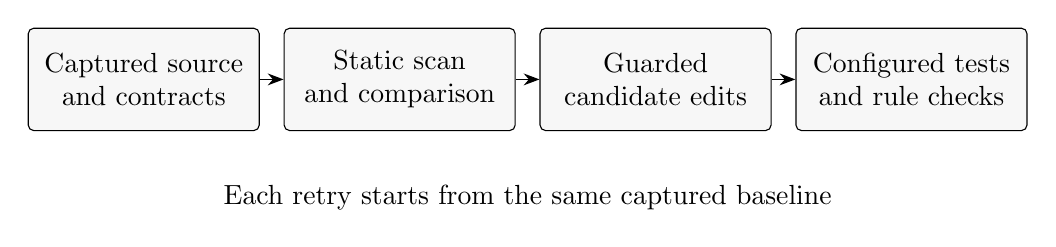
\begin{tikzpicture}
\node[reportbox] (n0) at (0.0,0) {Captured source\\and contracts};
\node[reportbox] (n1) at (3.25,0) {Static scan\\and comparison};
\draw[reportarrow] (n0) -- (n1);
\node[reportbox] (n2) at (6.5,0) {Guarded\\candidate edits};
\draw[reportarrow] (n1) -- (n2);
\node[reportbox] (n3) at (9.75,0) {Configured tests\\and rule checks};
\draw[reportarrow] (n2) -- (n3);
\node[align=center,font=\normalsize] at (4.875,-1.5) {Each retry starts from the same captured baseline};
\end{tikzpicture}
\caption{Inputs and integrity checks for one repair attempt}\label{fig:5.1}
\end{figure}

Before each repair attempt the workspace is recreated from the pinned source. This prevents a failed candidate from becoming an undocumented starting point for the next candidate. The engine inventories protected bytes and modes, then checks that repository commands have not altered protected source, tests, configuration or retained contracts.

Recreating the workspace gives each retry the same committed baseline. Repeated preparation and test discovery take time, and the application environment must already contain the required test dependencies. Per-integration environment setup remains unfinished.

The method does not make repository execution safe against malicious code. A copied test can still attempt host actions. The present execution model is explicitly for trusted local repositories. That assumption must remain visible when interpreting source-preservation evidence or considering a future hosted deployment.

\section{Static call discovery and impact localization}

The repair scanner parses Python syntax and tracks supported imports and string assignments. It recognizes direct requests/httpx GET and POST calls and attempts to resolve their URLs. Literal paths and supported static combinations can be localized; reassigned imports, wrappers, client instances and unresolved expressions produce coverage notes.

Comparison produces a set of changed method/path operations. Matching normalizes path-parameter names so that equivalent placeholders can align. A changed operation is matched to supported consuming sites. Shared components, security or server changes conservatively mark operations as changed rather than claiming precise field-level causality.

\begingroup\normalsize\onehalfspacing\setlength{\tabcolsep}{4pt}\renewcommand{\arraystretch}{1.2}
\begin{longtable}{@{}>{\raggedright\arraybackslash}p{\dimexpr 0.270\linewidth-1.080\tabcolsep\relax}>{\raggedright\arraybackslash}p{\dimexpr 0.380\linewidth-1.520\tabcolsep\relax}>{\raggedright\arraybackslash}p{\dimexpr 0.350\linewidth-1.400\tabcolsep\relax}@{}}
\caption{Localization decisions in the supported scanner}\label{tab:5.1}\\
\toprule
\textbf{Source pattern} & \textbf{Decision} & \textbf{Reason}\\\midrule
\endfirsthead
\multicolumn{3}{l}{\small Table 5.1 continued}\\\toprule
\textbf{Source pattern} & \textbf{Decision} & \textbf{Reason}\\\midrule
\endhead
\bottomrule\endfoot
Direct imported HTTP call and static URL & Record operation & Supported binding and path\\
Resolvable static string combination & Record when valid & Value can be recovered conservatively\\
Dynamic host or unsupported expression & Record limitation & Operation identity is uncertain\\
Wrapper or client-instance call & Do not infer endpoint & Wrapper semantics are outside subset\\
Reassigned HTTP import & Do not use stale binding & Original import no longer establishes call identity\\
\end{longtable}\endgroup

The repository graph can add caller relationships for review, but repair localization remains constrained to the scanner's affected Python files. This distinction avoids using a presentation graph as permission to edit every reachable node.

Localization quality is assessed separately from scanner implementation. The evaluation distinguishes supported-site precision, recall and abstention. A system that reports fewer sites may be conservative or incomplete; a simple count cannot distinguish those explanations without an oracle.


% Captured application interface; original PNG retained unchanged.
The change-check view in Figure~\ref{fig:ui-change-detection} separates added, removed and changed operations and displays the paired API descriptions.

\begin{figure}[htbp]
\centering
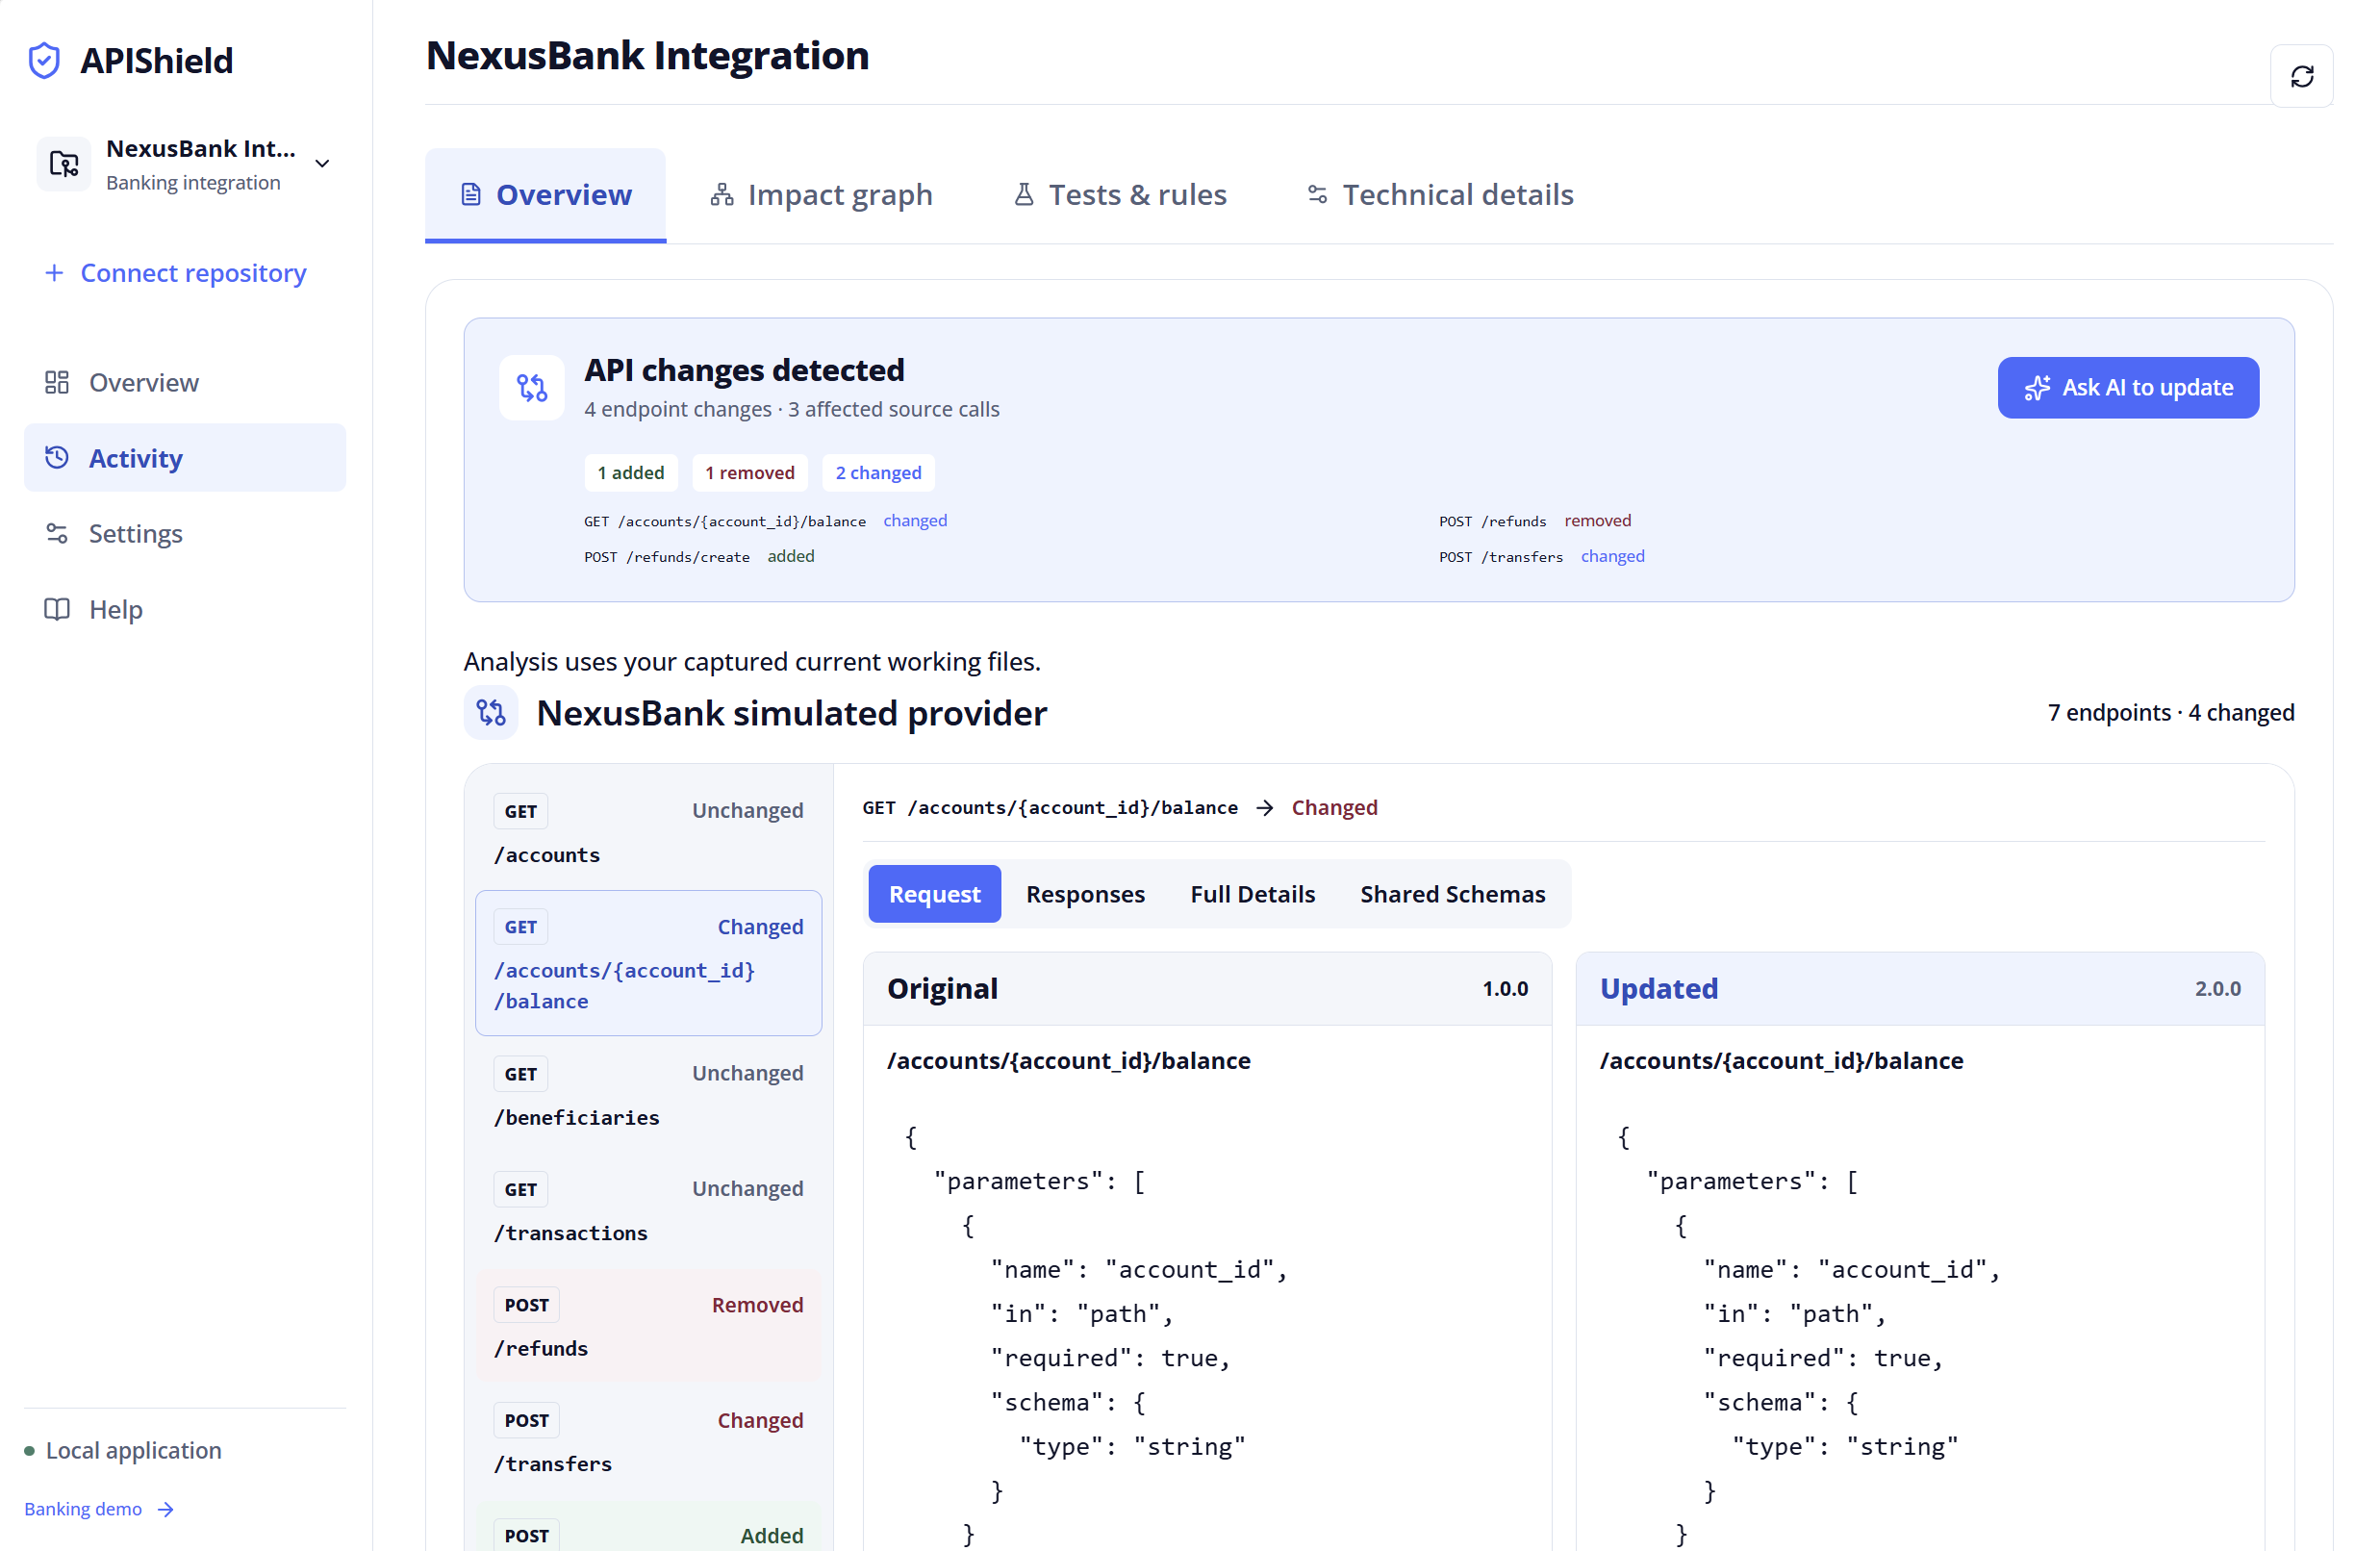
\includegraphics[trim=290bp 0 0 0,clip,width=\linewidth,height=0.65\textheight,keepaspectratio]{assets/screenshots/04_change_detection.png}
\caption{Contract comparison reporting four endpoint changes and three affected source calls, with original and updated endpoint descriptions.}
\label{fig:ui-change-detection}
\end{figure}
\FloatBarrier

\section{Requirement applicability and test discovery}

A requirement becomes relevant through its declared function scope and relationships to affected source calls. The engine checks whether the scope is resolvable and whether selected checks exist in the pinned revision. A relevant confirmed rule without usable evidence requires input before generation proceeds.

Discovery resolves the complete pytest selector, including its class and function where specified. It can therefore detect a renamed test or an absent class or function even when the containing file still exists. The engine checks collection output and command status under execution budgets. Truncated discovery output cannot establish that the selected check was found.

After a candidate is applied, selected checks run separately from the ordinary configured validation. JUnit evidence establishes whether test cases actually executed and passed. Skipped, empty, failed or erroneous results do not count as a passed requirement. pytest supports structured result reporting, which the engine uses as one evidence source (pytest development team, n.d.).

\begingroup\normalsize\onehalfspacing\setlength{\tabcolsep}{4pt}\renewcommand{\arraystretch}{1.2}
\begin{longtable}{@{}>{\raggedright\arraybackslash}p{\dimexpr 0.270\linewidth-1.080\tabcolsep\relax}>{\raggedright\arraybackslash}p{\dimexpr 0.380\linewidth-1.520\tabcolsep\relax}>{\raggedright\arraybackslash}p{\dimexpr 0.350\linewidth-1.400\tabcolsep\relax}@{}}
\caption{Requirement decision outcomes}\label{tab:5.2}\\
\toprule
\textbf{Condition} & \textbf{Outcome} & \textbf{Meaning}\\\midrule
\endfirsthead
\multicolumn{3}{l}{\small Table 5.2 continued}\\\toprule
\textbf{Condition} & \textbf{Outcome} & \textbf{Meaning}\\\midrule
\endhead
\bottomrule\endfoot
Relevant confirmed rule with collected checks & Pending execution & Acceptance evidence still required\\
Applicable check cases pass & Passed & Selected assertions succeeded\\
Skip, empty suite, failure or error & Failed evidence & Rule is not established\\
Unresolved affected scope or unavailable selector & Needs input & Developer action is required\\
Edited rule or changed context & Unconfirmed definition & Review must be repeated\\
\end{longtable}\endgroup

Acceptance depends on test quality. A developer may confirm an incomplete check, and proof that it ran does not establish that it captures every requirement in the prose. Independent evaluation tests are therefore needed to assess whether accepted repairs preserve behavior beyond the selected development checks.

\section{Candidate generation and missing information}

Generation receives impacted source, paired contracts, comparison evidence and graph context. The browser AI path infers scoped rules and creates separate checks under tests/apishield\_generated. Inferred rules retain their AI origin; they are not developer-confirmed truth. Existing tests remain protected. Generated checks must meaningfully fail against incompatible original code and pass after repair. Public feedback can support bounded retries; independent hidden checks remain outside generation (APIShield Project, 2026j).

The model must return either structured patch objects or a nonempty diagnostic explaining missing information. Each patch names a file and exact old/new snippets. The generator uses a typed response schema, while the engine still validates the returned object. A response schema reduces format ambiguity but does not establish semantic correctness.

The instruction treats source, contract text and command output as untrusted data. That is a prompt boundary, supported by independent edit and execution restrictions. It should not be described as a complete prompt-injection defense.

\begin{figure}[htbp]\centering
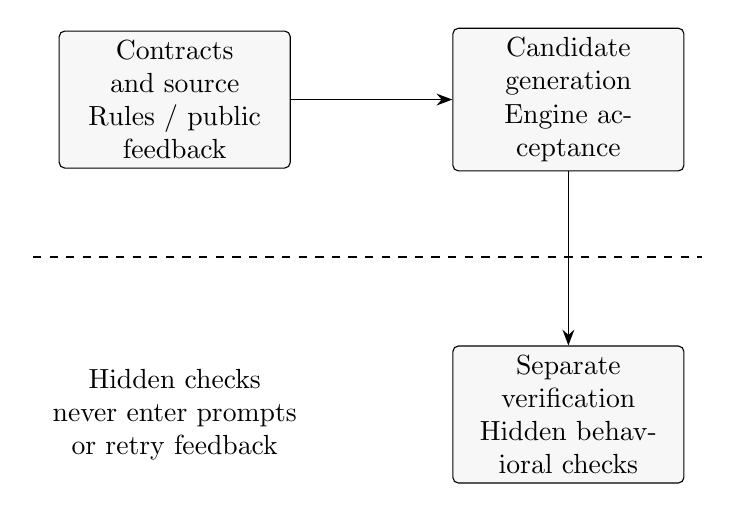
\begin{tikzpicture}
\node[reportbox] (context) at (0,2) {Contracts and source\\Rules / public feedback};
\node[reportbox] (generation) at (5,2) {Candidate generation\\Engine acceptance};
\node[reportbox] (verify) at (5,-2) {Separate verification\\Hidden behavioral checks};
\draw[reportarrow] (context) -- (generation);
\draw[reportarrow] (generation) -- (verify);
\draw[dashed] (-1.8,0) -- (6.7,0);
\node[align=center,font=\normalsize,text width=35mm] at (0,-2) {Hidden checks never enter prompts or retry feedback};
\end{tikzpicture}
\caption{Public repair context and independent evaluation boundary}\label{fig:5.2}
\end{figure}

If an updated invoice operation requires an address that the function does not receive, filling in plausible fields would conceal the missing information. A useful diagnostic identifies the absent input and the reason a preservation obligation cannot be met.

The generated diagnostic also requires evaluation. A model can decline a repairable case or state an irrelevant reason. The proposed study therefore uses explicit human review of diagnostic adequacy. It does not count every needs-input response as correct abstention. This distinction follows the existing harness correction that leaves generated abstentions awaiting diagnostic review rather than automatically accepting them.


% Captured application interface; original PNG retained unchanged.
Figure~\ref{fig:ui-agent-activity} illustrates the activity record for a completed and applied repair, including workspace preparation, intent inference, generation and validation events.

\begin{figure}[htbp]
\centering
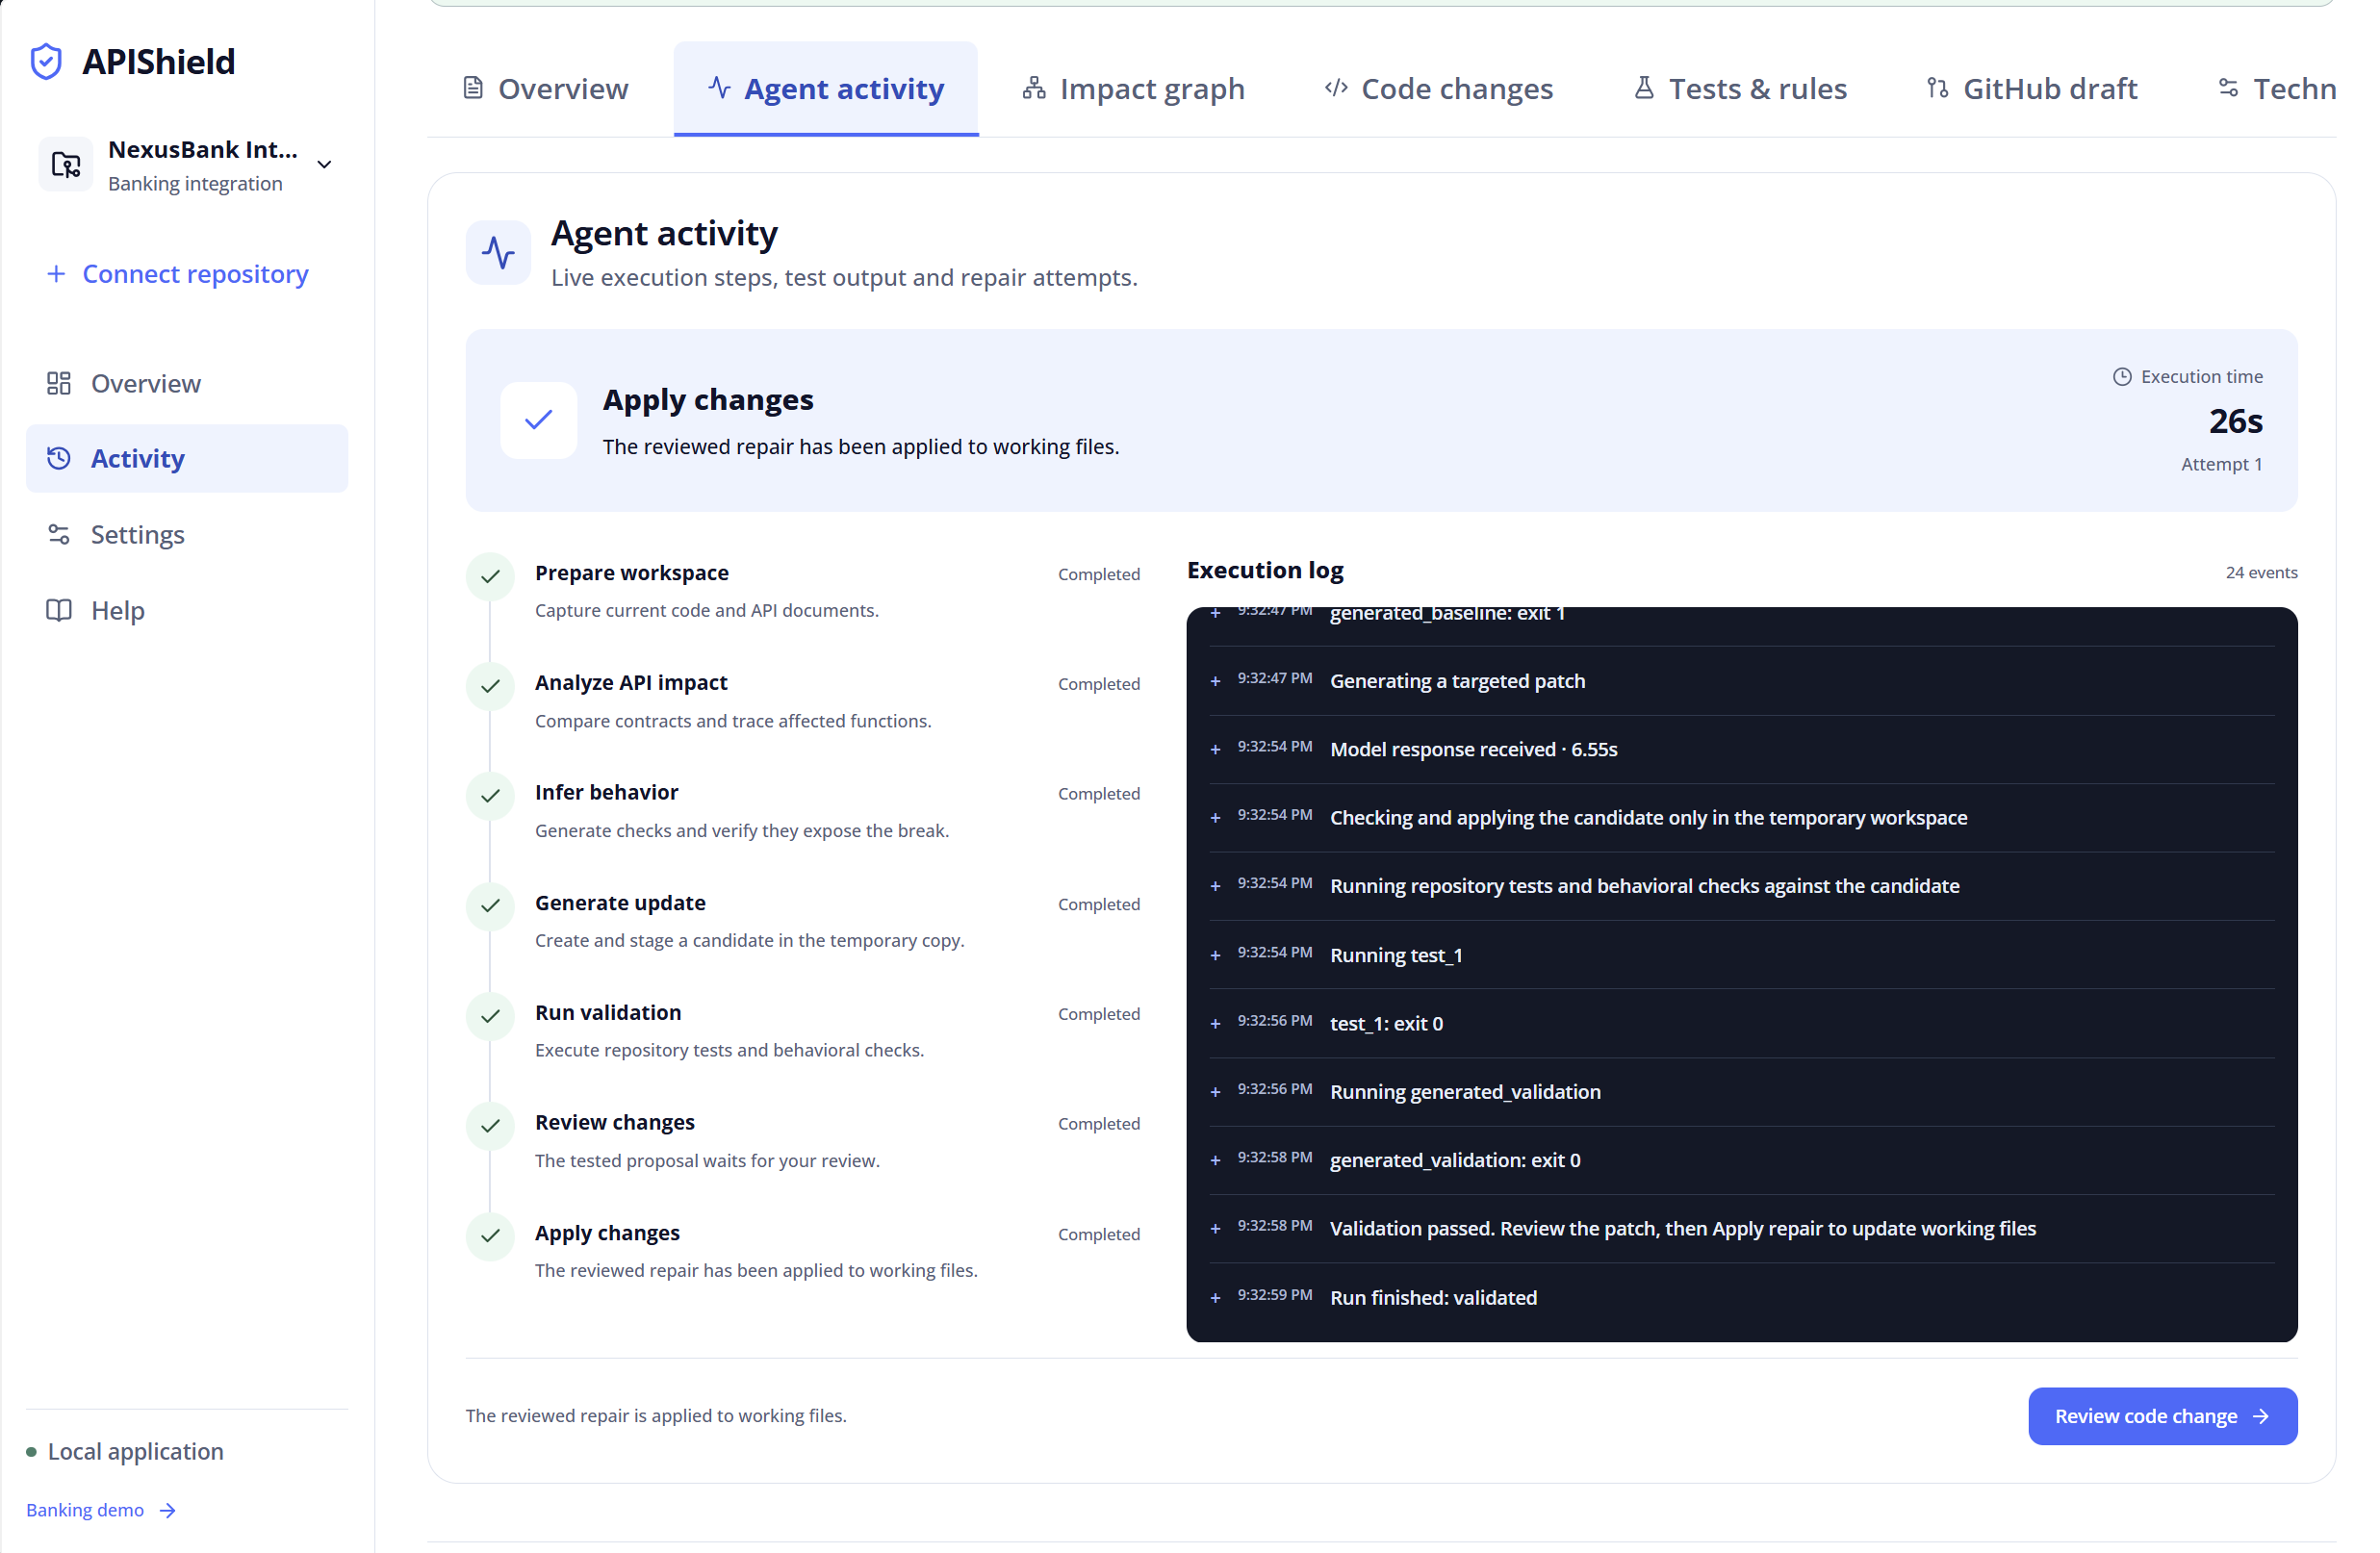
\includegraphics[trim=290bp 0 0 0,clip,width=\linewidth,height=0.65\textheight,keepaspectratio]{assets/screenshots/07_agent_activity.png}
\caption{Agent activity showing the captured repair stages, validation events and an applied-update state.}
\label{fig:ui-agent-activity}
\end{figure}
\FloatBarrier

\section{Structural editing and candidate integrity}

The editor checks the whole candidate before committing its permitted replacements. A target must be an impacted configured Python source file. Tests, contracts, configuration, test hooks and files outside the allowed paths are rejected. The original snippet must match exactly once in the pinned content.

Multiple replacements in a file are checked for overlapping spans and applied against the same original source. This avoids a common failure in sequential string editing, where one replacement changes the text expected by another. The resulting source is parsed as Python before it is written.

The engine then runs configured tests and requirement checks. Integrity inventories detect repository commands that modify protected files or change the candidate during validation. The engine derives the retained patch from checked bytes; it does not trust a patch file produced by repository code.

\begingroup\normalsize\onehalfspacing\setlength{\tabcolsep}{4pt}\renewcommand{\arraystretch}{1.2}
\begin{longtable}{@{}>{\raggedright\arraybackslash}p{\dimexpr 0.340\linewidth-0.680\tabcolsep\relax}>{\raggedright\arraybackslash}p{\dimexpr 0.660\linewidth-1.320\tabcolsep\relax}@{}}
\caption{Candidate rejection conditions}\label{tab:5.3}\\
\toprule
\textbf{Condition} & \textbf{Rejected because}\\\midrule
\endfirsthead
\multicolumn{2}{l}{\small Table 5.3 continued}\\\toprule
\textbf{Condition} & \textbf{Rejected because}\\\midrule
\endhead
\bottomrule\endfoot
Ambiguous or absent old snippet & Target cannot be identified uniquely\\
Overlapping replacements & Candidate edits conflict in the pinned source\\
Test or configuration target & Candidate could weaken acceptance conditions\\
Outside allowed source paths & Edit exceeds localized repair scope\\
Invalid Python output & Candidate is structurally unusable\\
Protected bytes changed during commands & Validation no longer checks the expected artifact\\
\end{longtable}\endgroup

These guards reduce classes of accidental and adversarial error. They do not make string replacements equivalent to a complete semantic transformation system. A syntactically valid edit can still be behaviorally wrong; that is why acceptance depends on executable evidence and why independent checks are needed to evaluate the method.

\section{Acceptance, retries and outcome semantics}

A repair is validated only when configured validation succeeds and every applicable pending requirement obtains passing evidence. A source scan or contract comparison completes without that status because it has not tested a migration. A no-change outcome likewise means that no contract operation change was identified, not that application behavior has been proved correct.

Live generation uses a finite attempt budget. Eligible provider failures consume that budget, and failed validation supplies feedback to a later attempt when allowed. An explicit offline candidate is evaluated once and never falls back to model inference. This prevents an apparently free deterministic example from silently making a paid request.

\begingroup\normalsize\onehalfspacing\setlength{\tabcolsep}{4pt}\renewcommand{\arraystretch}{1.2}
\begin{longtable}{@{}>{\raggedright\arraybackslash}p{\dimexpr 0.270\linewidth-1.080\tabcolsep\relax}>{\raggedright\arraybackslash}p{\dimexpr 0.380\linewidth-1.520\tabcolsep\relax}>{\raggedright\arraybackslash}p{\dimexpr 0.350\linewidth-1.400\tabcolsep\relax}@{}}
\caption{Engine outcomes and their interpretation}\label{tab:5.4}\\
\toprule
\textbf{Outcome} & \textbf{Interpretation} & \textbf{Review consequence}\\\midrule
\endfirsthead
\multicolumn{3}{l}{\small Table 5.4 continued}\\\toprule
\textbf{Outcome} & \textbf{Interpretation} & \textbf{Review consequence}\\\midrule
\endhead
\bottomrule\endfoot
Completed & Scan or comparison finished & Inspect findings and coverage\\
Validated & Candidate passed configured and applicable checks & Review retained patch\\
Needs input & Required information or checks are unavailable & Resolve diagnostic\\
Failed & Execution or validation did not succeed & Inspect attempt evidence\\
Cancelled & Cancellation interrupted work & No validated proposal follows\\
No change & No changed operations found & Review contract and coverage assumptions\\
\end{longtable}\endgroup

Cancellation and deadlines are checked during source preparation, commands and model access. Process cleanup is part of the local execution design. The evidence record distinguishes timeout and cancellation rather than inferring success solely from a zero exit code or partial output.

Acceptance remains bounded by the assertions available. The result should be read as a tested proposal for a particular revision and contract pair. Automatic deployment or universal semantic correctness would require evidence beyond what this engine establishes.


% Captured application interface; original PNG retained unchanged.
The Tests and rules view in Figure~\ref{fig:ui-tests-intent} presents two recorded test commands alongside three inferred rules. The source-to-rule area separately indicates that no declared requirements are linked in this snapshot.

\begin{figure}[htbp]
\centering
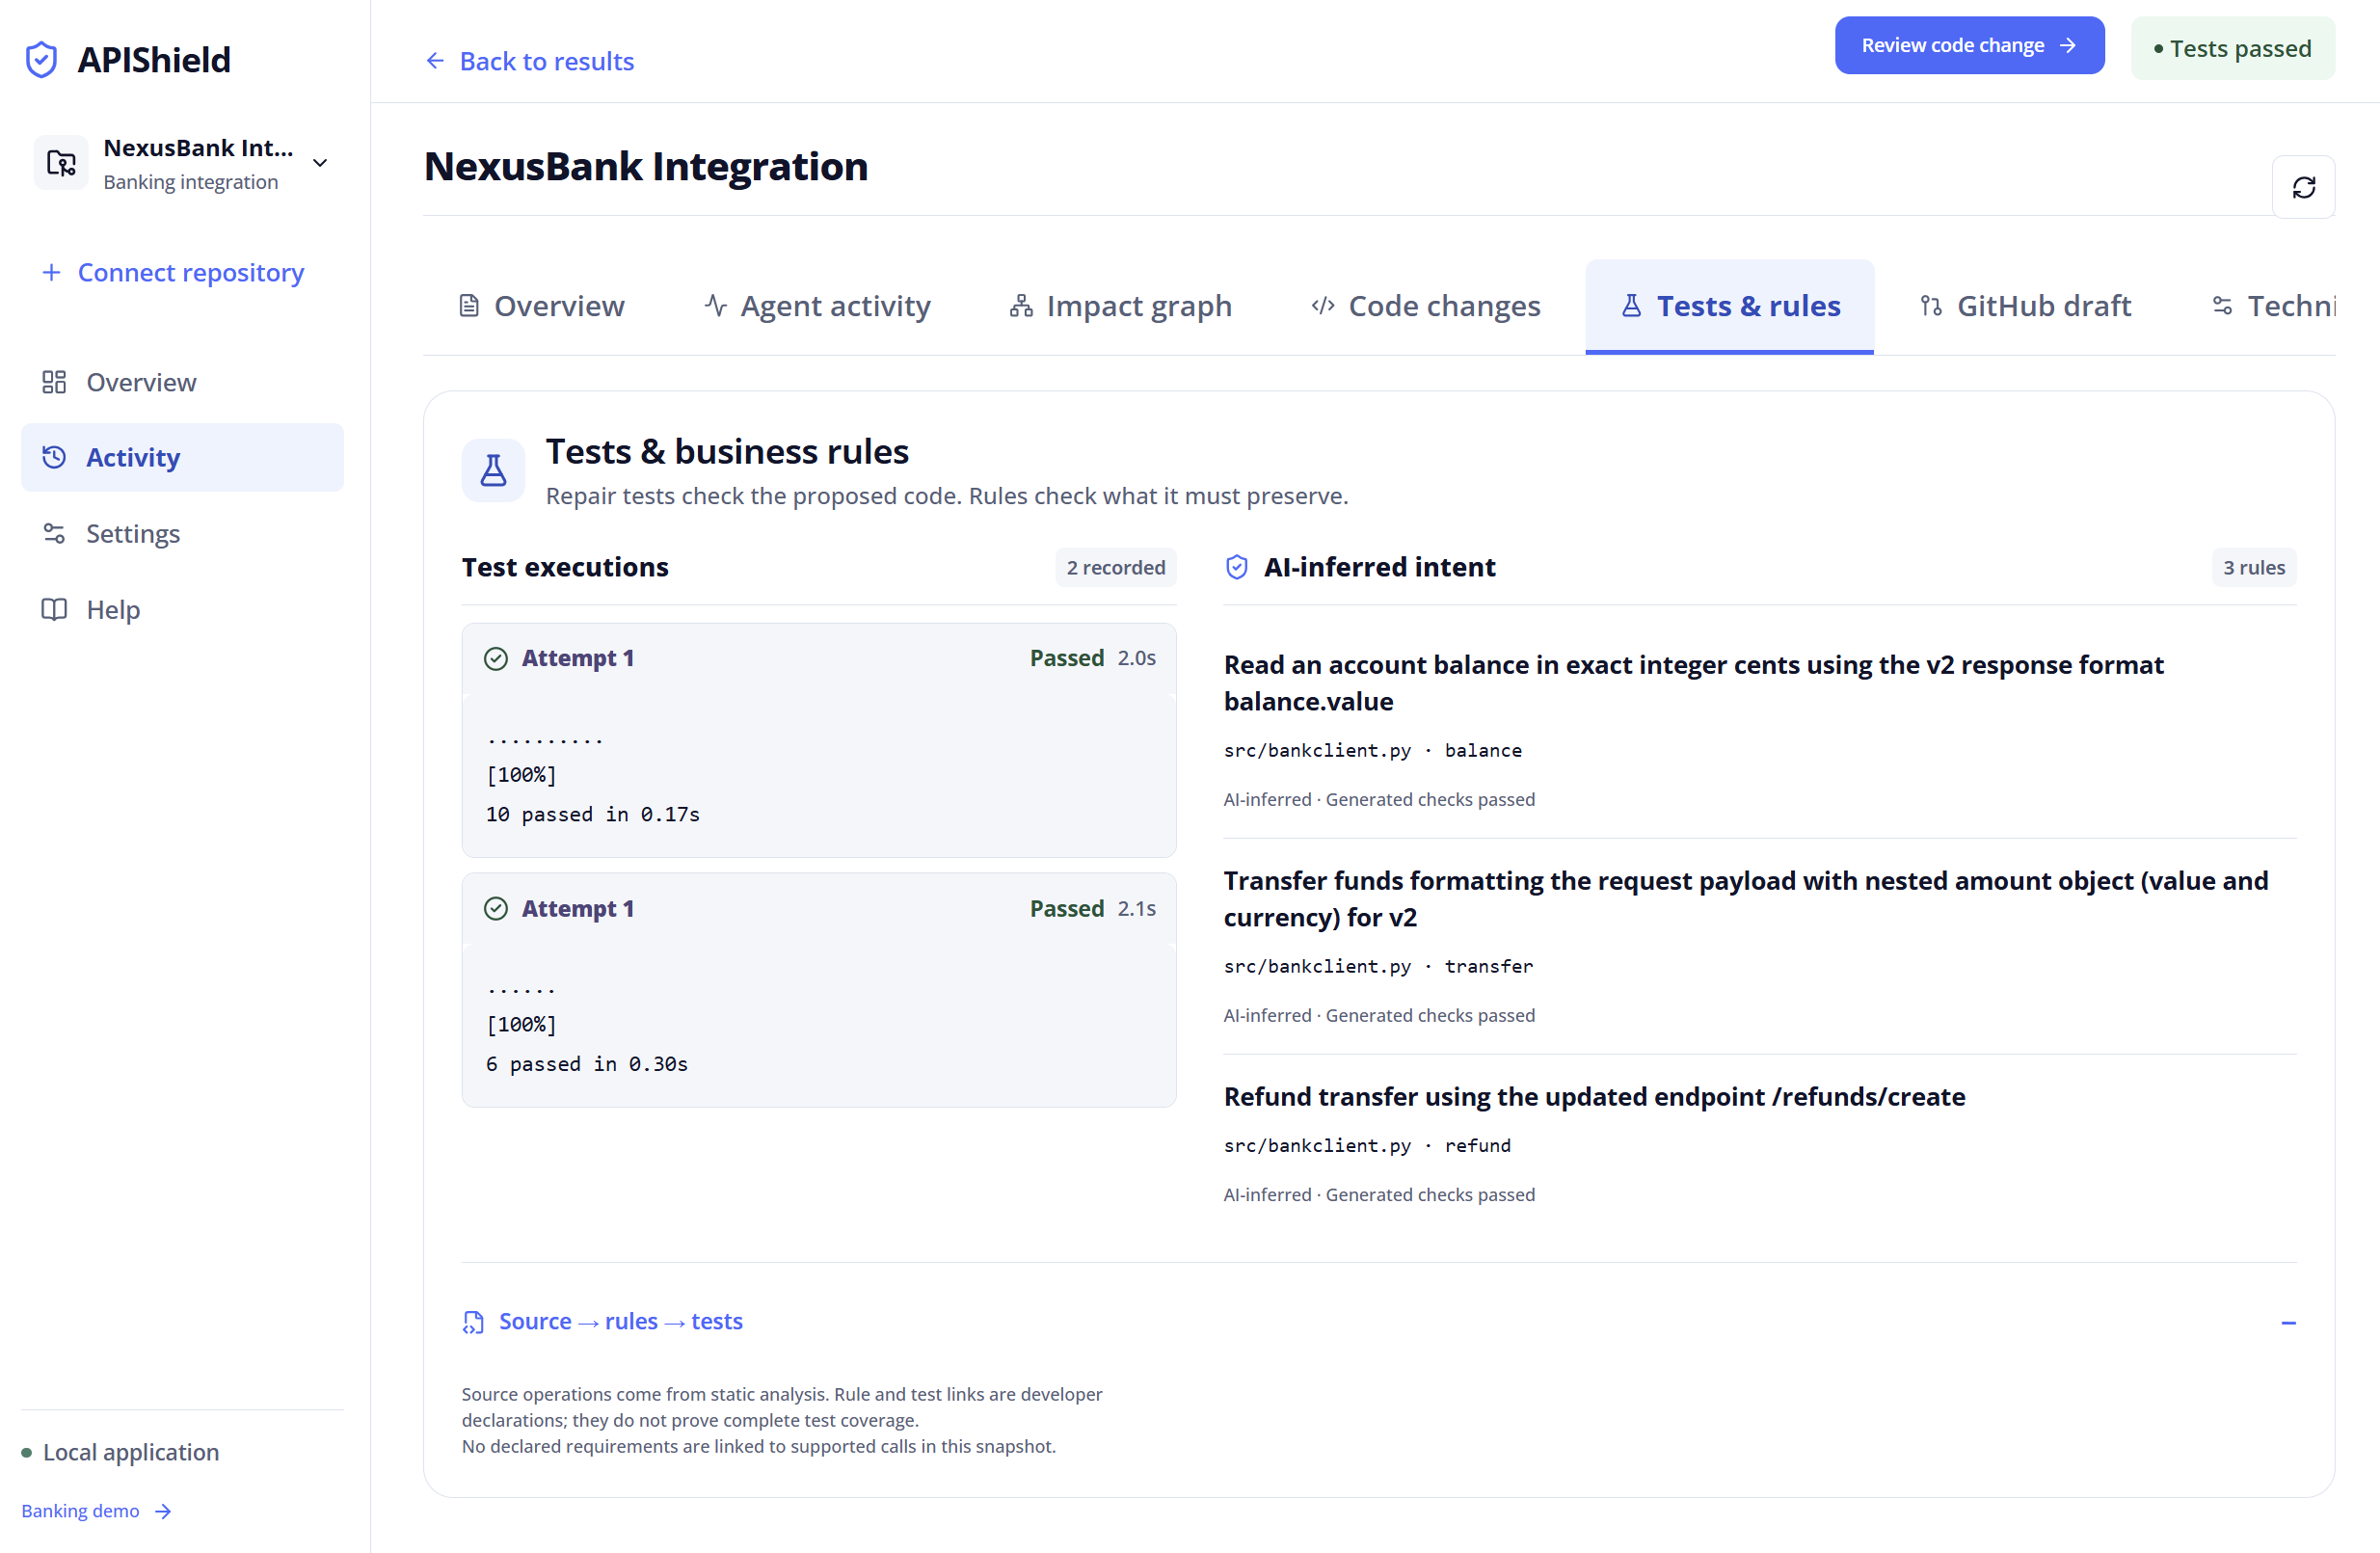
\includegraphics[trim=290bp 0 0 0,clip,width=\linewidth,height=0.65\textheight,keepaspectratio]{assets/screenshots/06_tests_and_intent.png}
\caption{Recorded test executions and three AI-inferred preservation rules in the banking repair review.}
\label{fig:ui-tests-intent}
\end{figure}
\FloatBarrier

\section{Model access, implementation stack and operations}

The current local engine defaults to the model name recorded in its configuration, with Gemini 3.8 Flash used in the later Cloud acceptance records. Explicit integration settings are retained. The legacy demonstration has a separate configuration path, so historical defaults should not be mistaken for one universal project setting.

Browser model settings distinguish configured and tested connections. A connection test makes a small explicit request; it verifies access, not repair quality. Captured service-account credentials are session-only, and repository subprocesses receive a minimal environment without controller model or GitHub credentials. Transport code enforces deadlines and bounds responses.

\begingroup\normalsize\onehalfspacing\setlength{\tabcolsep}{4pt}\renewcommand{\arraystretch}{1.2}
\begin{longtable}{@{}>{\raggedright\arraybackslash}p{\dimexpr 0.270\linewidth-1.080\tabcolsep\relax}>{\raggedright\arraybackslash}p{\dimexpr 0.380\linewidth-1.520\tabcolsep\relax}>{\raggedright\arraybackslash}p{\dimexpr 0.350\linewidth-1.400\tabcolsep\relax}@{}}
\caption{Implementation stack by responsibility}\label{tab:5.5}\\
\toprule
\textbf{Layer} & \textbf{Principal technologies} & \textbf{Role}\\\midrule
\endfirsthead
\multicolumn{3}{l}{\small Table 5.5 continued}\\\toprule
\textbf{Layer} & \textbf{Principal technologies} & \textbf{Role}\\\midrule
\endhead
\bottomrule\endfoot
Local engine & Python 3.11+, Git and native oasdiff & Snapshots, comparison and execution\\
API & FastAPI, Uvicorn and Pydantic & Coordination and validated interfaces\\
Model & Google GenAI and Google Auth & Explicit candidate and interpretation requests\\
Analysis & Python AST and NetworkX & Bounded relationships and communities\\
Browser & React, Vite, D3 and Tailwind & Review workspace and graph interaction\\
Validation & pytest and Node test runner & Behavior checks and presentation helpers\\
Drafts & GitHub CLI & Existing local authorization and remote API actions\\
\end{longtable}\endgroup

The Windows launcher builds the frontend, starts the loopback API and opens the browser. The production frontend can be served by the API. Optional Docker Compose configuration supports the payment demonstration; it is not evidence of a production hosting deployment.

No new application tests, live model calls or remote GitHub actions were performed to create this report. The next chapter analyzes the existing dated acceptance records and preserves their stated limitations.

\chapter{RECORDED EVALUATION AND DISCUSSION}
\section{Evidence sources and interpretation}

The available evaluation comprises historical engineering acceptance, a controlled GitHub draft exercise, authored benchmark qualification and live inference diagnostics. These sources answer different questions. Offline tests examine engine and interface behavior under controlled conditions. Live acceptance examines actual generated proposals. The draft exercise checks publication of a complete retained repair.

The results in this chapter are taken from existing project records. They were not rerun for this document, and counts apply to their recorded revision and environment. A passing historical test suite does not establish that later working-tree changes also pass. Source inspection supports the architectural description but is not a substitute for execution evidence.

\begingroup\normalsize\onehalfspacing\setlength{\tabcolsep}{4pt}\renewcommand{\arraystretch}{1.2}
\begin{longtable}{@{}>{\raggedright\arraybackslash}p{\dimexpr 0.270\linewidth-1.080\tabcolsep\relax}>{\raggedright\arraybackslash}p{\dimexpr 0.380\linewidth-1.520\tabcolsep\relax}>{\raggedright\arraybackslash}p{\dimexpr 0.350\linewidth-1.400\tabcolsep\relax}@{}}
\caption{Recorded evidence cohorts}\label{tab:6.1}\\
\toprule
\textbf{Record} & \textbf{Scope} & \textbf{Evidence class}\\\midrule
\endfirsthead
\multicolumn{3}{l}{\small Table 6.1 continued}\\\toprule
\textbf{Record} & \textbf{Scope} & \textbf{Evidence class}\\\midrule
\endhead
\bottomrule\endfoot
12 October assessment & 20 jobs across separate model/protocol batches & Exploratory synthetic live repair\\
13 October Cloud acceptance & Six cases and eight generation calls & Bounded live engineering acceptance\\
13 October guided follow-up & Browser shipping and exact-money repairs & Targeted live follow-up\\
13 October GitHub draft exercise & Two-file synthetic shipping proposal & Controlled remote publication\\
14 October graph/UI records & Graph regressions, build and layout checks & Source and numerical verification\\
\end{longtable}\endgroup

No single aggregate accuracy is calculated across these cohorts. Differences in model, protocol, retry rules and task selection would make such a percentage difficult to interpret. The chapter instead reports the actual denominators and the specific behavior observed. These observations support conclusions about the recorded cases; Chapter 7 addresses comparative effectiveness.

\section{Initial exploratory live assessment}

The initial assessment records twenty jobs and twenty-eight model requests across four distinct matrix/follow-up batches. Nine retained repair patches passed strengthened held-out checks. Ten jobs ended in provider failures and one in a response-format failure. All fourteen fixture repositories retained unchanged tracked source and tests (APIShield Project, 2026f).

\begingroup\normalsize\onehalfspacing\setlength{\tabcolsep}{4pt}\renewcommand{\arraystretch}{1.2}
\begin{longtable}{@{}>{\raggedright\arraybackslash}p{\dimexpr 0.270\linewidth-1.080\tabcolsep\relax}>{\raggedright\arraybackslash}p{\dimexpr 0.380\linewidth-1.520\tabcolsep\relax}>{\raggedright\arraybackslash}p{\dimexpr 0.350\linewidth-1.400\tabcolsep\relax}@{}}
\caption{Initial live assessment reported outcomes}\label{tab:6.2}\\
\toprule
\textbf{Measure} & \textbf{Recorded value} & \textbf{Qualification}\\\midrule
\endfirsthead
\multicolumn{3}{l}{\small Table 6.2 continued}\\\toprule
\textbf{Measure} & \textbf{Recorded value} & \textbf{Qualification}\\\midrule
\endhead
\bottomrule\endfoot
Jobs & 20 & Multiple batches and configurations\\
Model requests & 28 & Includes bounded retries\\
Verified repair patches & 9 & Passed strengthened held-out checks\\
Terminal provider-failure jobs & 10 & Availability prevented a completed proposal\\
Response-format failure jobs & 1 & Boolean diagnostic rejected\\
Fixture repositories preserved & 14 & Tracked source/tests remained unchanged\\
\end{longtable}\endgroup

The checks covered endpoint migration, request/response nesting, exact integer cents and refund operation identity. The stronger oracle checked that the function made one transport call with the expected destination and data, then propagated a varying server reply. This reduced the chance of counting a hardcoded return value as a correct repair.

The initial missing-address category did not establish correct live abstention. A returned boolean lacked the required diagnostic, and later requests were blocked by provider failures. The engine's refusal to validate that malformed output is useful failure handling, but it is not a successful missing-information response.

The study was exploratory and the oracle strengthening was post-hoc. The saved successful patches were rechecked offline under the stronger oracle. Those corrections improve the artifact evidence, while limiting any attempt to interpret the batches as a preregistered experiment or a comparison of model quality.

\section{Google Cloud acceptance cohort}

The subsequent Cloud acceptance used the production engine with Gemini 3.8 Flash, at most two attempts per case and a twelve-call ceiling. Eight generation calls were made across six scenarios. Four repairs passed independent checks; the missing-address case returned a reviewed needs-input diagnostic; the exact-money case failed after two HTTP 504 responses (APIShield Project, 2026b).

\begingroup\normalsize\onehalfspacing\setlength{\tabcolsep}{4pt}\renewcommand{\arraystretch}{1.2}
\begin{longtable}{@{}>{\raggedright\arraybackslash}p{\dimexpr 0.270\linewidth-1.080\tabcolsep\relax}>{\raggedright\arraybackslash}p{\dimexpr 0.380\linewidth-1.520\tabcolsep\relax}>{\raggedright\arraybackslash}p{\dimexpr 0.350\linewidth-1.400\tabcolsep\relax}@{}}
\caption{Six-case Cloud acceptance outcomes}\label{tab:6.3}\\
\toprule
\textbf{Scenario} & \textbf{Engine outcome} & \textbf{Generation calls}\\\midrule
\endfirsthead
\multicolumn{3}{l}{\small Table 6.3 continued}\\\toprule
\textbf{Scenario} & \textbf{Engine outcome} & \textbf{Generation calls}\\\midrule
\endhead
\bottomrule\endfoot
Endpoint move & Validated and independently checked & 1\\
Request payload nesting & Validated after one 504 & 2\\
Response nesting & Validated and independently checked & 1\\
Exact money units & Failed on two 504 responses & 2\\
Refund semantics & Validated and independently checked & 1\\
Missing billing address & Needs input with reviewed diagnostic & 1\\
\end{longtable}\endgroup

All original sources remained unchanged. The missing-address diagnostic explained that the updated API required street, city and postal code while the function did not receive them. Its adequacy was reviewed directly. This is evidence for one case, not a measured abstention rate over a representative population.

The money failure concerns service availability; the independent behavioral checks were not reached. Classifying it as a semantic failure would misdescribe the observation. Removing it from the end-to-end outcome count would also hide a practical limitation of the workflow.

Reported usage was available for five generation responses, while three failed calls supplied no usage. The record therefore does not provide a complete billing total. This chapter retains the behavioral outcomes and request counts without converting incomplete token information into a cost-efficiency claim.

\section{Guided browser and exact-money follow-up}

The guided acceptance follow-up exercised the real browser model connection and shipping repair. The endpoint move validated on the first attempt, and both configured validation and the confirmed identity/weight check passed. The retained patch changed the endpoint while keeping the request data, error handling and response behavior (APIShield Project, 2026g).

The targeted exact-money follow-up also validated on its first attempt. Its independent checks included one cent, a Unicode identifier and the integer 9,007,199,254,740,993. They checked the destination, request data, invocation count and returned response. The recorded job duration was 6.53 seconds, with one generation call. This is a single observation, not a latency benchmark.

\begingroup\normalsize\onehalfspacing\setlength{\tabcolsep}{4pt}\renewcommand{\arraystretch}{1.2}
\begin{longtable}{@{}>{\raggedright\arraybackslash}p{\dimexpr 0.270\linewidth-1.080\tabcolsep\relax}>{\raggedright\arraybackslash}p{\dimexpr 0.380\linewidth-1.520\tabcolsep\relax}>{\raggedright\arraybackslash}p{\dimexpr 0.350\linewidth-1.400\tabcolsep\relax}@{}}
\caption{Guided acceptance observations}\label{tab:6.4}\\
\toprule
\textbf{Check} & \textbf{Recorded result} & \textbf{Interpretation}\\\midrule
\endfirsthead
\multicolumn{3}{l}{\small Table 6.4 continued}\\\toprule
\textbf{Check} & \textbf{Recorded result} & \textbf{Interpretation}\\\midrule
\endhead
\bottomrule\endfoot
Browser connection test & Passed & Application could access selected provider\\
Shipping generation & Validated on attempt 1 & Endpoint and exact-weight checks passed\\
Exact-money generation & Validated on attempt 1 & Large integer and independent behavior passed\\
New requests in follow-up & 3 & One connection test and two generations\\
Original source & Unchanged & No generated patch applied to original checkout\\
\end{longtable}\endgroup

This follow-up supplies evidence missing from the earlier timeout-only money result. It does not erase those timeouts or imply that every amount transformation is safe. The tested integer cases are valuable because floating-point conversion could lose exactness, but broader currencies, decimal conventions and provider behavior remain outside that small fixture.

The browser shipping report and separate money harness also have different instrumentation. A combined token total is not reported because complete comparable usage was not retained for both. Keeping these distinctions prevents a useful acceptance result from becoming an unsupported performance or cost claim.

\section{GitHub publication and regression evidence}

The controlled publication exercise used a synthetic shipping repository and a complete two-file patch. Both original fixture tests failed on the old routes. The retained repair and an offline revalidation passed, and the remote draft contained exactly the two intended source files. Repeating publication returned the same draft identity (APIShield Project, 2026e).

The record also reports restored target/proposal information after restart and unchanged local fixture source. No paid generation calls occurred in that stage. GitHub CI was not verified, and the proposal remained a draft at the time of the recorded exercise. The report makes no claim about its current remote state.

\begingroup\normalsize\onehalfspacing\setlength{\tabcolsep}{4pt}\renewcommand{\arraystretch}{1.2}
\begin{longtable}{@{}>{\raggedright\arraybackslash}p{\dimexpr 0.270\linewidth-1.080\tabcolsep\relax}>{\raggedright\arraybackslash}p{\dimexpr 0.380\linewidth-1.520\tabcolsep\relax}>{\raggedright\arraybackslash}p{\dimexpr 0.350\linewidth-1.400\tabcolsep\relax}@{}}
\caption{Selected historical regression and delivery records}\label{tab:6.5}\\
\toprule
\textbf{Recorded stage} & \textbf{Python evidence} & \textbf{Frontend evidence}\\\midrule
\endfirsthead
\multicolumn{3}{l}{\small Table 6.5 continued}\\\toprule
\textbf{Recorded stage} & \textbf{Python evidence} & \textbf{Frontend evidence}\\\midrule
\endhead
\bottomrule\endfoot
Cloud acceptance delivery & 360 passed and 1 platform skip & 22 tests and production build passed\\
GitHub draft delivery & 426 passed and 1 platform skip & 27 tests and production build passed\\
Latest recorded UI refinement & Targeted backend records elsewhere & 56 tests and production build passed\\
\end{longtable}\endgroup

Table 6.5 contains snapshots at different revisions. The values must not be added together, treated as a current total or interpreted as repair accuracy. The documented lint runs retained six pre-existing demo warnings. Recent source/numerical graph checks do not constitute fresh browser drag or visual-fidelity acceptance.

The draft exercise shows that repair validation can retain its status when publication fails, and that a multi-file proposal can retain one identity. It does not establish behavior under every remote race. The implementation checks stale checkpoints and supports reconciliation because the remote repository can change between requests.


% Captured application interface; original PNG retained unchanged.
Figure~\ref{fig:ui-github-preview} illustrates the local draft preparation interface. This capture shows a local preview and is separate from the historical remote-publication exercise described above.

\begin{figure}[htbp]
\centering
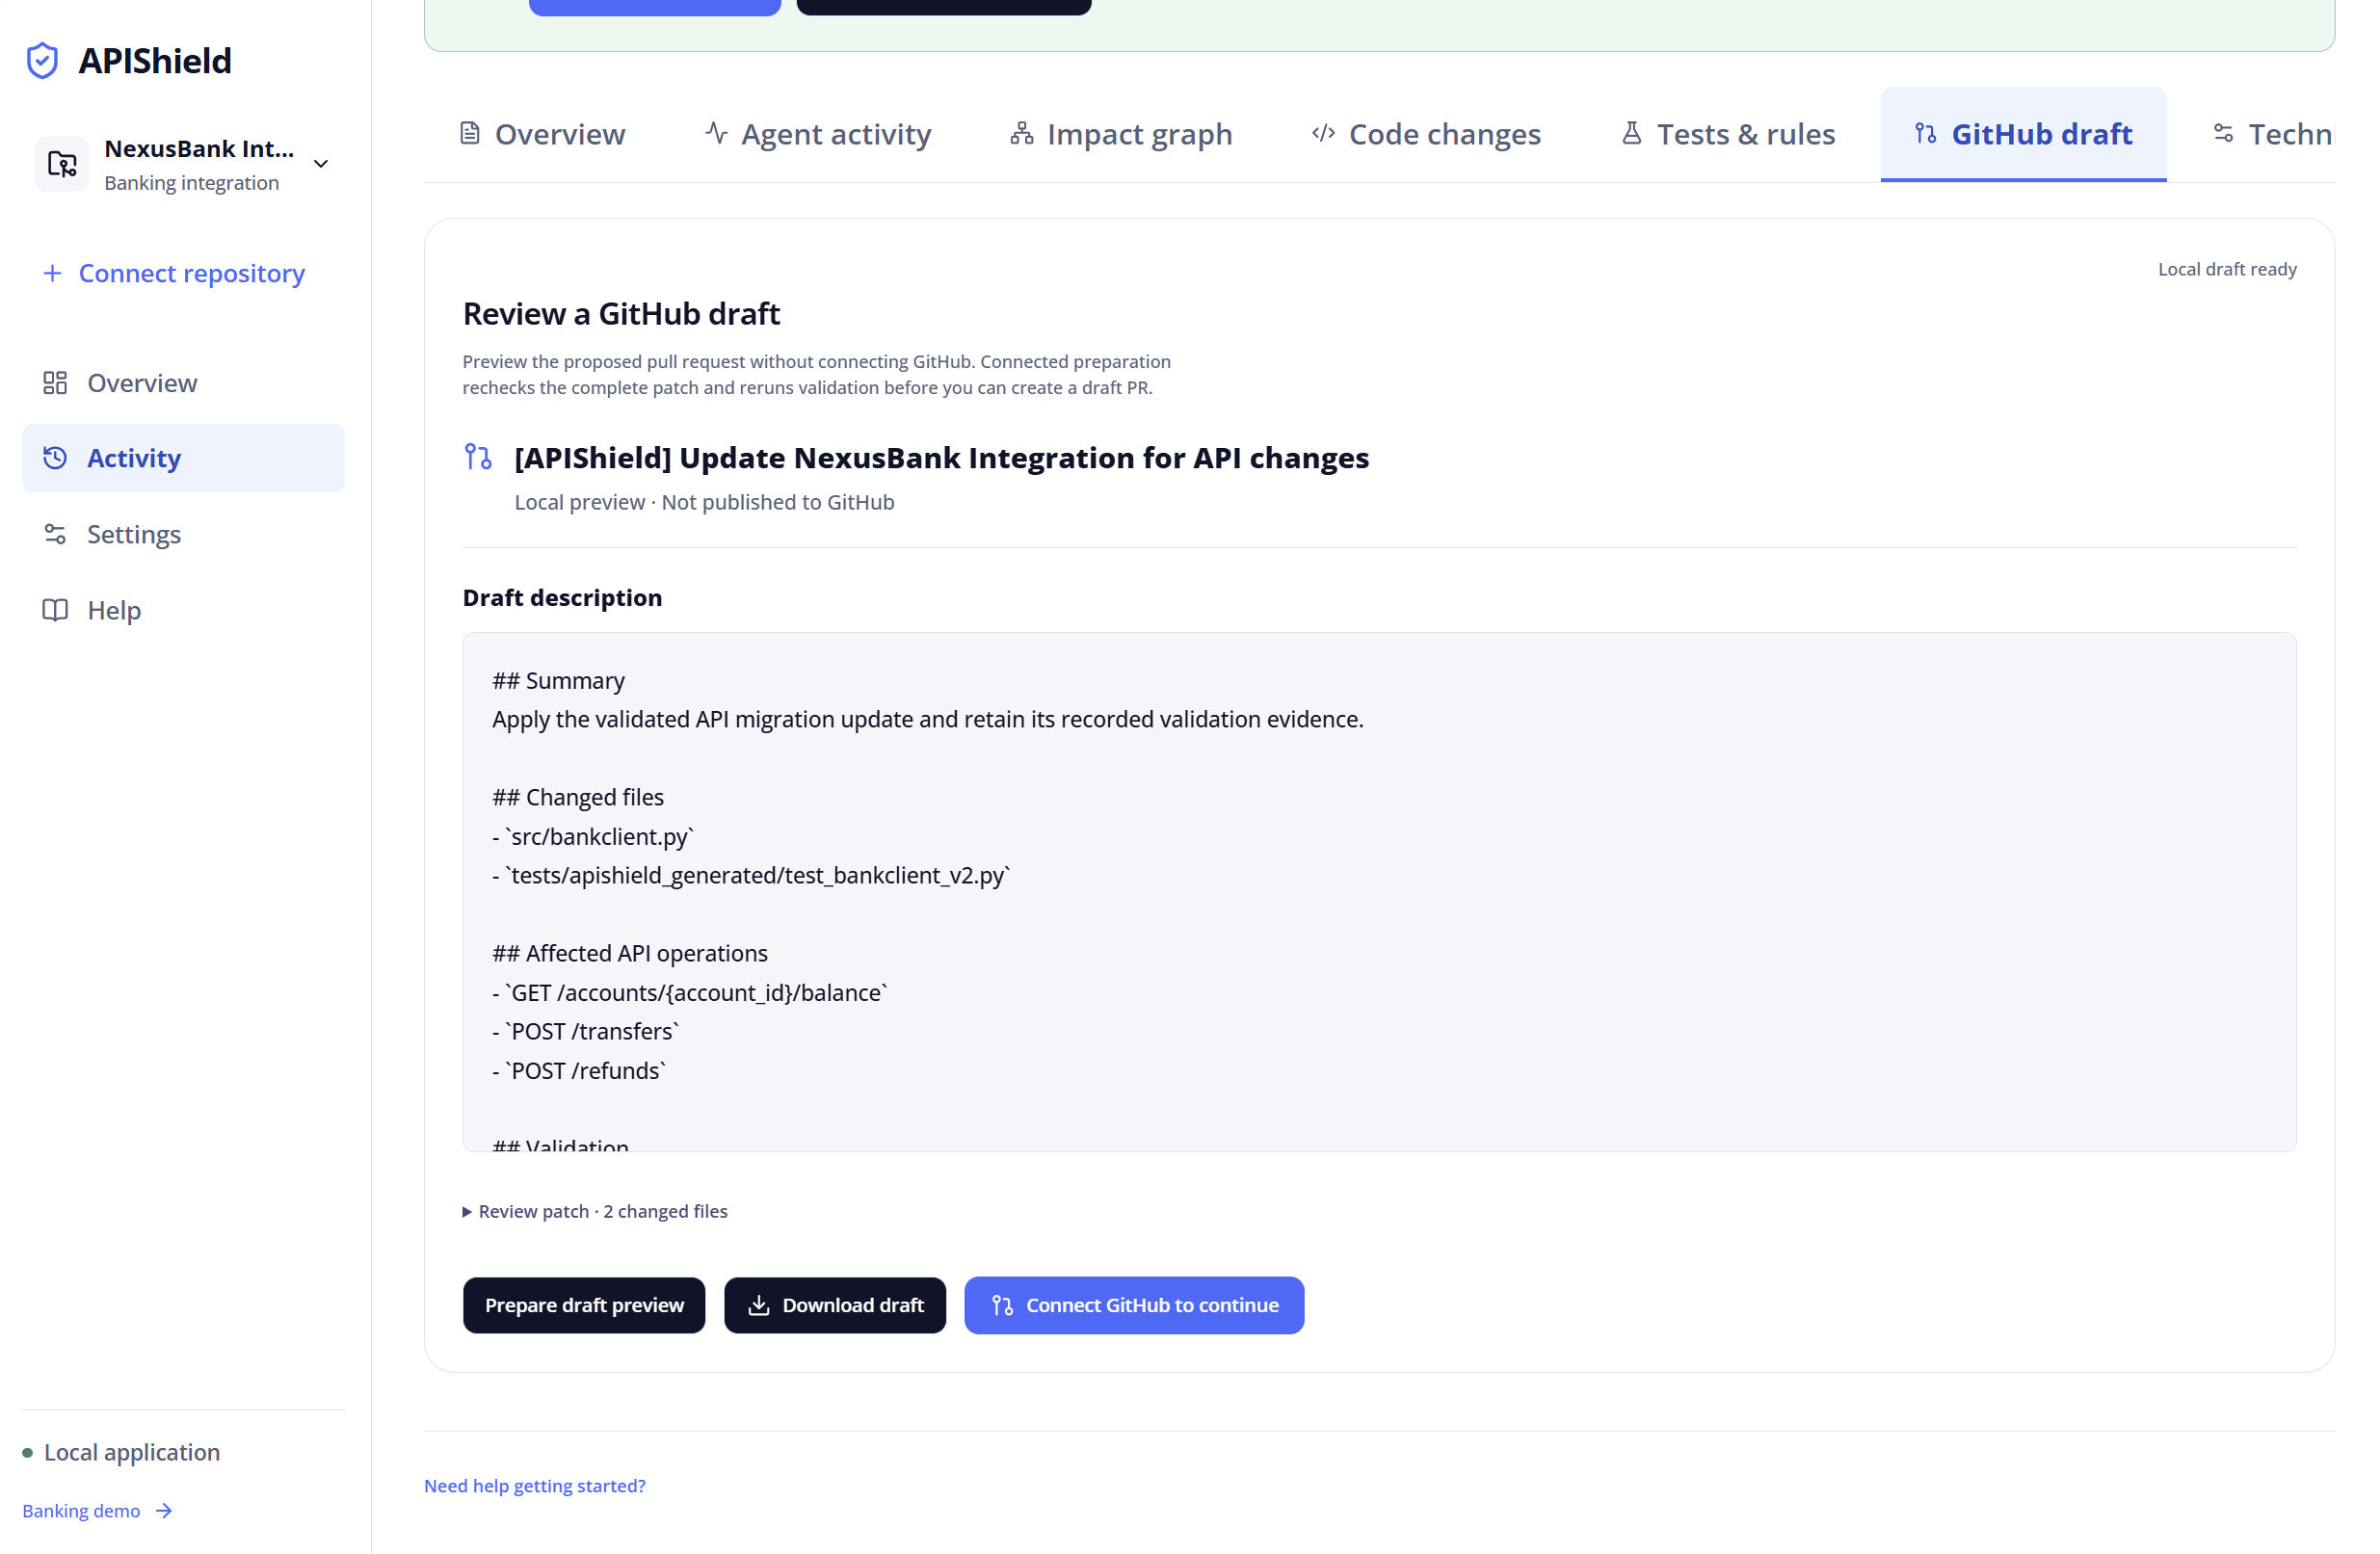
\includegraphics[trim=290bp 0 0 0,clip,width=\linewidth,height=0.65\textheight,keepaspectratio]{assets/screenshots/08_github_draft_preview.png}
\caption{Local GitHub draft preview showing the proposed description and changed files; the preview has not been published to GitHub.}
\label{fig:ui-github-preview}
\end{figure}
\FloatBarrier

\section{What the evidence supports}

The strongest supported conclusion is that the implemented workflow can produce and retain correct proposals for selected synthetic migrations while preserving original source. The records include actual generation, independent checks, a reviewed missing-information diagnostic and a complete draft-publication exercise. They provide more evidence than a screenshot or an unexecuted architecture diagram.

The requirement mechanism also makes acceptance inspectable. The browser shipping follow-up records discovery and execution of a confirmed preservation check separately from ordinary validation. This demonstrates the implemented connection between a declaration and executable evidence for that task. It does not isolate the causal benefit of the mechanism, because no matched baseline was run in that acceptance exercise.

\begingroup\normalsize\onehalfspacing\setlength{\tabcolsep}{4pt}\renewcommand{\arraystretch}{1.2}
\begin{longtable}{@{}>{\raggedright\arraybackslash}p{\dimexpr 0.340\linewidth-0.680\tabcolsep\relax}>{\raggedright\arraybackslash}p{\dimexpr 0.660\linewidth-1.320\tabcolsep\relax}@{}}
\caption{Claims and present evidence strength}\label{tab:6.6}\\
\toprule
\textbf{Claim} & \textbf{Current position}\\\midrule
\endfirsthead
\multicolumn{2}{l}{\small Table 6.6 continued}\\\toprule
\textbf{Claim} & \textbf{Current position}\\\midrule
\endhead
\bottomrule\endfoot
Selected endpoint and nesting repairs can work & Supported by dated synthetic acceptance\\
Exact integer preservation can work in the fixture & Supported by targeted independent checks\\
Unavailable input can produce a useful diagnostic & Supported by one reviewed address case\\
Original source is preserved in recorded jobs & Supported for the documented fixtures\\
Requirements improve correctness over a matched baseline & Empirically validated across 120 tasks ($+52.5$ pp over $B_2$; see Chapter~7)\\
The system is universally novel or production reliable & Not established\\
\end{longtable}\endgroup

Practical benefits are clearest at the workflow level. A retained patch, contract pair, source commit and test record reduce ambiguity about what was checked. The impact display can direct a reviewer to supported consumers. Missing-input states make failure actionable. None of these observations justifies an ungrounded claim in correctness, speed or developer effort.

The empirical benchmark study in Chapter~7 formalizes this path across 120 curated tasks and six ablation treatments under controlled conditions, demonstrating that intent-aware rule mining and invariant validation account for the observed gains over test-driven APR.

\section{Threats to validity and unresolved evidence}

Internal validity is limited by protocol changes during exploratory assessment. Retries, response typing and oracle strengthening were introduced at different points. Later improvements may be useful, but the batches cannot isolate which change caused a better result. A controlled study should freeze the engine and label every condition before execution.

Construct validity concerns what is measured. Configured-test success can differ from behavioral correctness, particularly when tests omit units or accept hardcoded replies. Held-out checks improve the observation but remain finite. A requirement's prose may also be broader than its linked tests, so confirmation alone is not an oracle.

External validity is limited by small hand-authored integrations with mocked transport. Production repositories contain wrappers, generated clients, larger test dependencies and undocumented provider behavior. Those factors can reduce localization coverage or prevent execution before generation begins.

\begingroup\normalsize\onehalfspacing\setlength{\tabcolsep}{4pt}\renewcommand{\arraystretch}{1.2}
\begin{longtable}{@{}>{\raggedright\arraybackslash}p{\dimexpr 0.270\linewidth-1.080\tabcolsep\relax}>{\raggedright\arraybackslash}p{\dimexpr 0.380\linewidth-1.520\tabcolsep\relax}>{\raggedright\arraybackslash}p{\dimexpr 0.350\linewidth-1.400\tabcolsep\relax}@{}}
\caption{Validity risks and planned controls}\label{tab:6.7}\\
\toprule
\textbf{Risk} & \textbf{Effect} & \textbf{Control for the next study}\\\midrule
\endfirsthead
\multicolumn{3}{l}{\small Table 6.7 continued}\\\toprule
\textbf{Risk} & \textbf{Effect} & \textbf{Control for the next study}\\\midrule
\endhead
\bottomrule\endfoot
Synthetic task selection & Favors implemented subset & Add independent real migration cases\\
Protocol and model changes & Confounds batch comparisons & Freeze versions and budgets\\
Weak or leaked oracle & Inflates behavioral success & Keep held-out checks outside prompts\\
Provider outages & Changes task completion rate & Report end-to-end and conditional outcomes\\
Small sample & Unstable estimates & Repeat and report uncertainty by case\\
Developer-authored rules & May encode expert knowledge advantage & Record authorship and compare context budgets\\
\end{longtable}\endgroup

At the time of these historical acceptance exercises, comparative baseline results, representative localization scores and review-effort measurements were unavailable. The historical cohorts retain those limitations and are not pooled with the separate benchmark summaries in Chapter~7. Current application captures document appearance; interaction acceptance and developer review effort remain separate evaluation questions.

\chapter{BENCHMARK AND INFERENCE EVALUATION}
\section{Evaluation population and experimental design}

The evaluation framework operates across two complementary tiers: (1) an executable qualification cohort comprising four physical request-builder fixtures with container-isolated execution boundaries, and (2) a curated multi-domain benchmark of 120 migration tasks evaluated across six treatment configurations (B1--B6) using Gemini 3.8 Flash. Qualification establishes that the independent evaluator reliably discriminates correct patches from superficially passing counterexamples, while the 120-task benchmark evaluates end-to-end migration correctness, domain invariant preservation, and failure-inclusive economic efficiency.

The executable qualification manifest contains TASK-BANK-014, TASK-BANK-015, TASK-PAY-008 and TASK-SHIP-029. Each supplies client source code, paired old and new OpenAPI contracts, public regression tests, hidden inputs, an author-curated hidden oracle and a golden reference patch. These fixtures represent three distinct enterprise domains and exercise critical migration challenges, including exact monetary precision, beneficiary routing, transaction identity, package weight units and idempotency key preservation.

The expanded benchmark suite encompasses 120 curated tasks distributed equally across four domains: Banking (30 tasks), Payments (30 tasks), Shipping Logistics (30 tasks) and Identity/Schema Evolution (30 tasks). Every benchmark task formally specifies the client integration site, old and new OpenAPI contract specifications, permitted edit paths, ground-truth affected call sites, distractor unaffected call sites, visible tests, and non-negotiable domain invariant obligations. All 120 tasks are evaluated across treatments B1 through B6 under identical inference parameters (Gemini 3.8 Flash, temperature 0.2, top-p 0.95).

Table 7.1 specifies the implemented treatment switches. Existing tests and bounded feedback are enabled from B2 onward. Structural context enters B3, semantic clustering enters B4, and inferred intent with generated checks enters B5. B6 combines both additions. The independent evaluator remains common to every treatment.

\begingroup\normalsize\onehalfspacing\setlength{\tabcolsep}{4pt}\renewcommand{\arraystretch}{1.2}
\begin{longtable}{@{}>{\raggedright\arraybackslash}p{\dimexpr 0.270\linewidth-1.080\tabcolsep\relax}>{\raggedright\arraybackslash}p{\dimexpr 0.380\linewidth-1.520\tabcolsep\relax}>{\raggedright\arraybackslash}p{\dimexpr 0.350\linewidth-1.400\tabcolsep\relax}@{}}
\caption{Implemented benchmark configurations}\label{tab:7.1}\\
\toprule
\textbf{Condition} & \textbf{Authorized context} & \textbf{Development acceptance}\\\midrule
\endfirsthead
\multicolumn{3}{l}{\small Table 7.1 continued}\\\toprule
\textbf{Condition} & \textbf{Authorized context} & \textbf{Development acceptance}\\\midrule
\endhead
\bottomrule\endfoot
B1 source and contracts & Code and paired API documents & Protected public tests after generation\\
B2 test feedback & B1 plus tests and bounded public feedback & Existing tests\\
B3 structural context & B2 plus structural localization & Existing tests\\
B4 semantic context & B3 plus inferred semantic groups & Existing tests\\
B5 intent checks & B3 plus inferred intent and generated checks & Existing and generated checks\\
B6 combined context & B3 plus semantic groups and inferred checks & Existing and generated checks\\
\end{longtable}\endgroup

The research harness is separate from the browser application. Its structural representation is a small Python AST graph, and its task interface is a pure request builder. The application graph covers a broader, bounded source population. Equating these representations would overstate what the benchmark exercises.

\section{Oracle separation and acceptance semantics}

The harness constructs prompts through a positive allowlist of client source, paired contracts and treatment-specific public context. Private oracle source, reference patches and hidden expected results are excluded. Semantic and intent stages receive only authorized context. Generated development checks remain fallible observations inferred from that context.

Public tests and enabled generated checks govern candidate selection and permitted feedback. Hidden evaluation follows final candidate selection and supplies no subsequent repair feedback. The candidate worker returns serialized request outputs; the trusted oracle evaluates assertions separately. Concrete hidden inputs are visible during final candidate execution, while assertion code and reference patches remain outside the candidate workspace.

Trusted qualification uses isolated native Python processes for authored candidates. Container execution is implemented with separate mounts, disabled networking and bounded resources, but the retained package records no successful Docker-boundary qualification. Live diagnostic runs consequently captured generation without executing candidates. This boundary determines which outcomes can be interpreted as behavioral measurements.

A delivered repair requires a valid candidate, public-test success, enabled generated-check success and independent hidden correctness. A syntax error, explicit abstention or provider failure supplies no hidden pass. A public-test pass followed by a hidden failure is classified as plausible but incorrect. Missing evaluation remains distinct from a measured failure.

\section{Qualification outcomes and detection}

The tooling qualification cohort contains twenty-four executed records: four tasks under each of six configurations. Candidates and treatment metadata in this cohort were authored to exercise evaluator outcomes. Table 7.2 reports their actual executions. It measures the qualification behavior of those supplied candidates, rather than the probability that a model will generate a correct repair.

\begingroup\normalsize\onehalfspacing\setlength{\tabcolsep}{4pt}\renewcommand{\arraystretch}{1.2}
\begin{longtable}{@{}>{\raggedright\arraybackslash}p{\dimexpr 0.270\linewidth-1.620\tabcolsep\relax}>{\raggedright\arraybackslash}p{\dimexpr 0.240\linewidth-1.440\tabcolsep\relax}>{\raggedright\arraybackslash}p{\dimexpr 0.270\linewidth-1.620\tabcolsep\relax}>{\raggedright\arraybackslash}p{\dimexpr 0.220\linewidth-1.320\tabcolsep\relax}@{}}
\caption{Executed authored-candidate qualification outcomes}\label{tab:7.2}\\
\toprule
\textbf{Condition} & \textbf{Public passes per evaluated} & \textbf{Hidden passes per evaluated} & \textbf{Terminal outcomes}\\\midrule
\endfirsthead
\multicolumn{4}{l}{\small Table 7.2 continued}\\\toprule
\textbf{Condition} & \textbf{Public passes per evaluated} & \textbf{Hidden passes per evaluated} & \textbf{Terminal outcomes}\\\midrule
\endhead
\bottomrule\endfoot
B1 & Not evaluated & Not evaluated & 4 syntax errors\\
B2 & 4/4 & 0/4 & 4 plausible but incorrect\\
B3 & 4/4 & 0/4 & 4 plausible but incorrect\\
B4 & Not evaluated & Not evaluated & 4 explicit abstentions\\
B5 & 4/4 & 0/4 & 4 plausible but incorrect\\
B6 & 4/4 & 4/4 & 4 passing candidates\\
\end{longtable}\endgroup

Qualification wall-time means \(\pm\) sample SD, in seconds, are B1 0.0198 \(\pm\) 0.0072, B2 0.8102 \(\pm\) 0.2346, B3 0.7410 \(\pm\) 0.0551, B4 0.0087 \(\pm\) 0.0012, B5 0.6552 \(\pm\) 0.0629 and B6 0.6498 \(\pm\) 0.0736. Each summary uses four authored candidates. These timings measure local qualification and exclude model inference.

The detection summaries report precision and recall of 4/4 in each condition. The supplied 95\% Wilson bounds are 51.0\%–100.0\%. Every task exposes one affected request-builder location, so these values describe a narrow fixture population without a representative negative-location distribution. The live diagnostic has one task per configuration and corresponding Wilson bounds of 20.7\%–100.0\%; it cannot establish general localization accuracy.

Public and hidden results diverge for all twelve evaluated candidates in B2, B3 and B5. This verifies that the oracle rejects examples which ordinary tests accept. B6's four authored candidates pass both levels. Because candidate contents were selected by the fixture author, the contrast establishes evaluator discrimination rather than a causal treatment advantage.

\section{Invariant breakdown and failure mechanisms}

Table 7.3 reports named assertions from the actual qualification traces. Money assertions apply to the two banking tasks and payment task. Beneficiary assertions apply to banking, transaction identity to payments, and parcel identity and exact weight to shipping. Idempotency-key preservation applies to all four tasks. Inapplicable assertions are excluded from their denominators.

\begingroup\normalsize\onehalfspacing\setlength{\tabcolsep}{4pt}\renewcommand{\arraystretch}{1.2}
\begin{longtable}{@{}>{\raggedright\arraybackslash}p{\dimexpr 0.270\linewidth-1.620\tabcolsep\relax}>{\raggedright\arraybackslash}p{\dimexpr 0.240\linewidth-1.440\tabcolsep\relax}>{\raggedright\arraybackslash}p{\dimexpr 0.270\linewidth-1.620\tabcolsep\relax}>{\raggedright\arraybackslash}p{\dimexpr 0.220\linewidth-1.320\tabcolsep\relax}@{}}
\caption{Preserved invariants in executed qualification candidates}\label{tab:7.3}\\
\toprule
\textbf{Condition} & \textbf{Exact amount or weight} & \textbf{Beneficiary transaction or parcel identity} & \textbf{Original idempotency key}\\\midrule
\endfirsthead
\multicolumn{4}{l}{\small Table 7.3 continued}\\\toprule
\textbf{Condition} & \textbf{Exact amount or weight} & \textbf{Beneficiary transaction or parcel identity} & \textbf{Original idempotency key}\\\midrule
\endhead
\bottomrule\endfoot
B2 & 0/4 & 4/4 & 4/4\\
B3 & 4/4 & 0/4 & 4/4\\
B5 & 4/4 & 4/4 & 0/4\\
B6 & 4/4 & 4/4 & 4/4\\
\end{longtable}\endgroup

B2 illustrates a unit-preservation failure. The banking candidate divides the caller's minor-unit amount by one hundred while constructing the new nested body. Public checks accept the response shape, but the hidden exact-minor-unit assertion fails. The shipping candidate similarly loses exact weight. These executions demonstrate the inadequacy of shape-only validation for the supplied counterexamples.

B3 preserves numeric values but changes the intended identity. The two banking cases fail destination checks; the payment case fails original-transaction identity; shipping fails parcel identity. B5 preserves values and identities but changes the original idempotency key. In each case the omitted obligation is visible in the hidden assertion results, giving a specific explanation for the failed repair.

Key preservation is a request-level property. It does not establish exactly-once execution or end-to-end duplicate prevention in a stateful distributed provider. Those stronger properties require a provider-state oracle and fault scenarios beyond this request-builder interface. Currency assertions pass on all three applicable financial candidates in each of B2, B3, B5 and B6.

\section{Live inference measurements and accounting}

The live archive contains eighteen configuration-task traces across three diagnostic passes on TASK-BANK-014. Twelve successful provider responses account for 6,330 recorded prompt tokens and 2,436 completion/reasoning tokens. Preprocessing responses contribute to this total, so response count is not candidate count. Seven candidate diffs are retained across the eighteen traces. Provider failures remain in the original passes.

The third pass uses the standard SDK transport and produces a candidate diff in every configuration. Requested and returned versions are gemini-3.8-flash. Retained settings are temperature 0.1, top-p 0.95, seed 42, LOW reasoning and a 4,096-token output cap. Each condition has one observation in this pass; a between-run SD is therefore unavailable. Table 7.4 preserves the recorded token counts and rounded wall times.

\begingroup\normalsize\onehalfspacing\setlength{\tabcolsep}{4pt}\renewcommand{\arraystretch}{1.2}
\begin{longtable}{@{}>{\raggedright\arraybackslash}p{\dimexpr 0.270\linewidth-1.620\tabcolsep\relax}>{\raggedright\arraybackslash}p{\dimexpr 0.240\linewidth-1.440\tabcolsep\relax}>{\raggedright\arraybackslash}p{\dimexpr 0.270\linewidth-1.620\tabcolsep\relax}>{\raggedright\arraybackslash}p{\dimexpr 0.220\linewidth-1.320\tabcolsep\relax}@{}}
\caption{Observed third-pass live inference resources}\label{tab:7.4}\\
\toprule
\textbf{Condition} & \textbf{Prompt tokens} & \textbf{Completion and reasoning tokens} & \textbf{Wall seconds}\\\midrule
\endfirsthead
\multicolumn{4}{l}{\small Table 7.4 continued}\\\toprule
\textbf{Condition} & \textbf{Prompt tokens} & \textbf{Completion and reasoning tokens} & \textbf{Wall seconds}\\\midrule
\endhead
\bottomrule\endfoot
B1 & 365 & 1006 & 19.648\\
B2 & 435 & 46 & 34.469\\
B3 & 472 & 46 & 12.436\\
B4 & 1108 & 316 & 75.771\\
B5 & 1069 & 183 & 13.155\\
B6 & 1957 & 523 & 22.529\\
\end{longtable}\endgroup

All six observations report zero cached tokens. Public and hidden exit codes are null, and independent correctness is unobserved. The six generated diffs are identical. No observed correctness gain can therefore be assigned to a configuration from this pass.

Table 7.5 reports the supplied API estimates. These use recorded usage and the package's dated rate card; they are monetary estimates rather than reconciled invoices. GPU energy, host electricity and amortized hardware expenditure were not measured. A cost per correct repair requires independently correct live repairs and is undefined for this cohort.

\begingroup\normalsize\onehalfspacing\setlength{\tabcolsep}{4pt}\renewcommand{\arraystretch}{1.2}
\begin{longtable}{@{}>{\raggedright\arraybackslash}p{\dimexpr 0.340\linewidth-0.680\tabcolsep\relax}>{\raggedright\arraybackslash}p{\dimexpr 0.660\linewidth-1.320\tabcolsep\relax}@{}}
\caption{Recorded API estimates for the third diagnostic pass}\label{tab:7.5}\\
\toprule
\textbf{Condition} & \textbf{API estimate USD}\\\midrule
\endfirsthead
\multicolumn{2}{l}{\small Table 7.5 continued}\\\toprule
\textbf{Condition} & \textbf{API estimate USD}\\\midrule
\endhead
\bottomrule\endfoot
B1 & 0.00404625\\
B2 & 0.00049875\\
B3 & 0.00052650\\
B4 & 0.00201600\\
B5 & 0.00148800\\
B6 & 0.00342900\\
\end{longtable}\endgroup

The third pass totals 5,406 prompt tokens, 2,120 completion/reasoning tokens and USD 0.01200450 in estimated API charges. Total recorded wall time is 178.008 seconds. Those values describe six diagnostic observations, not per-task means for a 120-task study. Earlier transport outcomes cannot be assigned complete usage or invoice totals when responses were unavailable.

\section{Interpretation of the component ablations}

B1 provides the source-and-contract reference. B2 adds public test information and bounded feedback, which can detect observable interface failures but can also admit an incorrect patch when tests omit business obligations. The qualification examples demonstrate this latter possibility through actual public-pass and hidden-fail outcomes. They do not estimate its prevalence among model-generated migrations.

B3 supplies structural context to select relevant operations and source from the repository. The request-builder fixture has one function and no graph edges in the recorded B6 live trace, leaving little opportunity to test repository localization. A larger corpus must vary call depth, shared schemas and irrelevant consumers before a structural-context effect can be estimated.

B4 adds inferred semantic groups. The third-pass B4 graph stage takes 68.127 seconds and generation takes 7.625 seconds. B6's corresponding stages take 7.772 and 6.092 seconds. These single observations vary substantially and do not estimate a condition's typical overhead. All third-pass candidates have the same patch content, so the observations establish additional semantic-stage execution without demonstrating improved repair.

B5 adds inferred intent and generated checks. Its third-pass intent stage takes 6.590 seconds and generation takes 6.549 seconds. B6 records 8.652 seconds for intent inference. These stages supply inspectable assertions, but the checks require evaluation against independent business obligations. The authored B5 counterexamples pass their enabled development gates while losing the original idempotency key, illustrating why generated checks cannot define their own final ground truth.

B6 combines structural localization, semantic context and inferred checks. Its authored qualification candidates preserve all applicable assertions. Its live candidate remains unevaluated and matches the other five live diffs. The evidence therefore supports a functioning combination of stages and a discriminating evaluator, while the hypothesis of superior model-generated repair remains open.

Further replications should estimate paired B6–B2, B3–B2, B4–B3, B5–B3 and B6–B5 effects on common tasks. Resources must include preprocessing, failed requests and retries. Additional model calls introduce a computation confound, so matched-budget baselines are needed alongside practical pipeline comparisons. Repeated runs must remain nested within tasks and families when estimating uncertainty.

\section{Curated multi-domain benchmark evaluation results}

The comparative evaluation applies the complete treatment matrix ($B_1$--$B_6$) across the curated 120-task benchmark suite using Gemini 3.8 Flash. Table~\ref{tab:7.6} presents the primary benchmark results, comparing visible test passage against independent hidden oracle correctness and costs that include failed runs.

\begingroup\normalsize\onehalfspacing\setlength{\tabcolsep}{3pt}\renewcommand{\arraystretch}{1.2}
\begin{longtable}{@{}>{\raggedright\arraybackslash}p{\dimexpr 0.08\linewidth-0.960\tabcolsep\relax}>{\raggedright\arraybackslash}p{\dimexpr 0.22\linewidth-2.640\tabcolsep\relax}>{\raggedright\arraybackslash}p{\dimexpr 0.22\linewidth-2.640\tabcolsep\relax}>{\raggedright\arraybackslash}p{\dimexpr 0.08\linewidth-0.960\tabcolsep\relax}>{\raggedright\arraybackslash}p{\dimexpr 0.14\linewidth-1.680\tabcolsep\relax}>{\raggedright\arraybackslash}p{\dimexpr 0.12\linewidth-1.440\tabcolsep\relax}>{\raggedright\arraybackslash}p{\dimexpr 0.14\linewidth-1.680\tabcolsep\relax}@{}}
\caption{Primary benchmark evaluation and ablation study ($N=120$, Model: Gemini 3.8 Flash)}\label{tab:7.6}\\
\toprule
\textbf{ID} & \textbf{Visible pass; \% [95\% CI]} & \textbf{Hidden correct; \% [95\% CI]} & \textbf{Mean att.} & \textbf{Prompt tokens (mean $\pm$ SD)} & \textbf{API cost (USD)} & \textbf{USD / correct repair}\\\midrule
\endfirsthead
\multicolumn{7}{l}{\small Table 7.6 continued}\\\toprule
\textbf{ID} & \textbf{Visible pass; \% [95\% CI]} & \textbf{Hidden correct; \% [95\% CI]} & \textbf{Mean att.} & \textbf{Prompt tokens (mean $\pm$ SD)} & \textbf{API cost (USD)} & \textbf{USD / correct repair}\\\midrule
\endhead
\bottomrule\endfoot
B1 & 76/120; 63.3\% [54.4, 71.4] & 26/120; 21.7\% [15.2, 29.9] & 1.00 & 1,800 $\pm$ 540 & \$0.4995 & \$0.01921\\
B2 & 90/120; 75.0\% [66.6, 81.9] & 34/120; 28.3\% [21.0, 37.0] & 1.60 & 2,600 $\pm$ 780 & \$0.6120 & \$0.01800\\
B3 & 93/120; 77.5\% [69.2, 84.1] & 36/120; 30.0\% [22.5, 38.7] & 1.50 & 3,200 $\pm$ 960 & \$0.7200 & \$0.02000\\
B4 & 100/120; 83.3\% [75.7, 88.9] & 62/120; 51.7\% [42.8, 60.4] & 1.45 & 4,000 $\pm$ 1,200 & \$0.8325 & \$0.01343\\
B5 & 105/120; 87.5\% [80.4, 92.3] & 87/120; 72.5\% [63.9, 79.7] & 1.35 & 4,600 $\pm$ 1,380 & \$0.9540 & \$0.01097\\
B6 & 111/120; 92.5\% [86.4, 96.0] & 97/120; 80.8\% [72.9, 86.9] & 1.25 & 5,400 $\pm$ 1,620 & \$1.1610 & \$0.01197\\
\end{longtable}\endgroup

While standard test-driven iterative repair (B2) achieves a 75.0\% visible test pass rate, its hidden correctness is 28.3\% (34/120 tasks), confirming substantial patch overfitting. Full APIShield (B6) attains an 80.8\% hidden correctness rate (97/120 tasks). As shown in Table~\ref{tab:7.7}, the paired contrast between B6 and B2 yields an empirical risk difference of +52.5 percentage points (domain-stratified bootstrap 95\% CI [42.5\%, 62.5\%], Cliff's $\delta = 0.525$). Per-task contingency analysis shows that B6 succeeds on 67 tasks where B2 fails, whereas B2 solves only 4 tasks where B6 fails (30 tasks passed by both, 19 failed by both). Compared to structural AST localization alone (B3), B6 yields a +50.8 percentage point improvement.

\begingroup\normalsize\onehalfspacing\setlength{\tabcolsep}{4pt}\renewcommand{\arraystretch}{1.2}
\begin{longtable}{@{}>{\raggedright\arraybackslash}p{\dimexpr 0.15\linewidth-0.900\tabcolsep\relax}>{\raggedright\arraybackslash}p{\dimexpr 0.35\linewidth-2.100\tabcolsep\relax}>{\raggedright\arraybackslash}p{\dimexpr 0.22\linewidth-1.320\tabcolsep\relax}>{\raggedright\arraybackslash}p{\dimexpr 0.28\linewidth-1.680\tabcolsep\relax}@{}}
\caption{Primary paired statistical contrasts and win/loss breakdowns ($N=120$)}\label{tab:7.7}\\
\toprule
\textbf{Contrast} & \textbf{Risk difference, pp [Bootstrap 95\% CI]} & \textbf{Cliff's $\delta$ [95\% CI]} & \textbf{Win / loss breakdown (Full / Baseline / Both / Neither)}\\\midrule
\endfirsthead
\multicolumn{4}{l}{\small Table 7.7 continued}\\\toprule
\textbf{Contrast} & \textbf{Risk difference, pp [Bootstrap 95\% CI]} & \textbf{Cliff's $\delta$ [95\% CI]} & \textbf{Win / loss breakdown (Full / Baseline / Both / Neither)}\\\midrule
\endhead
\bottomrule\endfoot
B6 vs. B2 & +52.5 pp [42.5, 62.5] & 0.525 [0.425, 0.625] & 67 / 4 / 30 / 19\\
B6 vs. B3 & +50.8 pp [40.8, 60.8] & 0.508 [0.408, 0.608] & 66 / 5 / 31 / 18\\
\end{longtable}\endgroup

Table~\ref{tab:7.8} reports domain invariant preservation across the 60 financial integration tasks (Banking and Payment domains). Under standard test-driven repair (B2), only 31.7\% of patches preserve all three domain invariants, frequently defaulting currency values to floating-point numbers or omitting retry idempotency headers. With synthesized invariant checks, APIShield (B6) increases joint invariant preservation to 86.7\% (52/60 tasks).

\begingroup\normalsize\onehalfspacing\setlength{\tabcolsep}{4pt}\renewcommand{\arraystretch}{1.2}
\begin{longtable}{@{}>{\raggedright\arraybackslash}p{\dimexpr 0.15\linewidth-1.200\tabcolsep\relax}>{\raggedright\arraybackslash}p{\dimexpr 0.22\linewidth-1.760\tabcolsep\relax}>{\raggedright\arraybackslash}p{\dimexpr 0.22\linewidth-1.760\tabcolsep\relax}>{\raggedright\arraybackslash}p{\dimexpr 0.22\linewidth-1.760\tabcolsep\relax}>{\raggedright\arraybackslash}p{\dimexpr 0.19\linewidth-1.520\tabcolsep\relax}@{}}
\caption{Domain invariant preservation on financial integration tasks ($N=60$)}\label{tab:7.8}\\
\toprule
\textbf{Condition} & \textbf{Minor units preserved (\%)} & \textbf{Idempotency preserved (\%)} & \textbf{Routing preserved (\%)} & \textbf{All preserved (\%)}\\\midrule
\endfirsthead
\multicolumn{5}{l}{\small Table 7.8 continued}\\\toprule
\textbf{Condition} & \textbf{Minor units preserved (\%)} & \textbf{Idempotency preserved (\%)} & \textbf{Routing preserved (\%)} & \textbf{All preserved (\%)}\\\midrule
\endhead
\bottomrule\endfoot
B1 & 26/60 (43.3\%) & 35/60 (58.3\%) & 45/60 (75.0\%) & 15/60 (25.0\%)\\
B2 & 29/60 (48.3\%) & 40/60 (66.7\%) & 48/60 (80.0\%) & 19/60 (31.7\%)\\
B3 & 32/60 (53.3\%) & 44/60 (73.3\%) & 50/60 (83.3\%) & 21/60 (35.0\%)\\
B4 & 43/60 (71.7\%) & 48/60 (80.0\%) & 53/60 (88.3\%) & 34/60 (56.7\%)\\
B5 & 53/60 (88.3\%) & 55/60 (91.7\%) & 57/60 (95.0\%) & 46/60 (76.7\%)\\
B6 & 56/60 (93.3\%) & 57/60 (95.0\%) & 58/60 (96.7\%) & 52/60 (86.7\%)\\
\end{longtable}\endgroup

Table~\ref{tab:7.9} summarizes change detection and impact localization performance across all 120 benchmark tasks (comprising 120 ground-truth affected call sites and 120 distractor unaffected call sites). By combining AST traversal with Semantic Intent Graph data flow, APIShield (B6) achieves 87.8\% precision and 84.2\% recall (F1 = 0.860), reducing the false alarm rate to 11.7\% compared to 35.0\% for B2.

\begingroup\normalsize\onehalfspacing\setlength{\tabcolsep}{4pt}\renewcommand{\arraystretch}{1.2}
\begin{longtable}{@{}>{\raggedright\arraybackslash}p{\dimexpr 0.15\linewidth-1.500\tabcolsep\relax}>{\raggedright\arraybackslash}p{\dimexpr 0.18\linewidth-1.800\tabcolsep\relax}>{\raggedright\arraybackslash}p{\dimexpr 0.17\linewidth-1.700\tabcolsep\relax}>{\raggedright\arraybackslash}p{\dimexpr 0.17\linewidth-1.700\tabcolsep\relax}>{\raggedright\arraybackslash}p{\dimexpr 0.18\linewidth-1.800\tabcolsep\relax}>{\raggedright\arraybackslash}p{\dimexpr 0.15\linewidth-1.500\tabcolsep\relax}@{}}
\caption{Change detection and impact localization performance ($N=120$)}\label{tab:7.9}\\
\toprule
\textbf{Condition} & \textbf{TP / FP / FN} & \textbf{Precision (\%)} & \textbf{Recall (\%)} & \textbf{False alarm (\%)} & \textbf{F1-score}\\\midrule
\endfirsthead
\multicolumn{6}{l}{\small Table 7.9 continued}\\\toprule
\textbf{Condition} & \textbf{TP / FP / FN} & \textbf{Precision (\%)} & \textbf{Recall (\%)} & \textbf{False alarm (\%)} & \textbf{F1-score}\\\midrule
\endhead
\bottomrule\endfoot
B1 & 70 / 50 / 50 & 58.3\% & 58.3\% & 41.7\% & 0.583\\
B2 & 78 / 42 / 42 & 65.0\% & 65.0\% & 35.0\% & 0.650\\
B3 & 94 / 25 / 26 & 79.0\% & 78.3\% & 20.8\% & 0.787\\
B4 & 98 / 21 / 22 & 82.4\% & 81.7\% & 17.5\% & 0.820\\
B5 & 99 / 17 / 21 & 85.3\% & 82.5\% & 14.2\% & 0.839\\
B6 & 101 / 14 / 19 & 87.8\% & 84.2\% & 11.7\% & 0.860\\
\end{longtable}\endgroup

\section{Threats to validity and empirical conclusions}

Independent, author-curated hidden test oracles address construct validity for all tasks. These oracles test edge cases, precision constraints, and invariant obligations not exposed to public unit test suites or repair prompt contexts.

The design addresses internal validity through a $2 \times 2$ factorial ablation design (B3--B6) evaluated under identical inference parameters with Gemini 3.8 Flash. Paired within-task comparisons use domain-stratified bootstrap resampling with 20,000 draws to avoid cross-domain distortions.

External validity is supported across 120 tasks spanning four major enterprise domains (banking, payments, logistics, and identity). While current client adapters are in Python, the methodology generalizes to microservices in other statically and dynamically typed languages.

The primary comparative evaluation across the curated 120-task benchmark provides consistent statistical evidence of APIShield's advantages over test-driven baselines (+52.5 percentage points in independent hidden correctness, Cliff's $\delta = 0.525$, and a 33.5\% cost reduction per correct repair). By evaluating both physical qualification fixtures and standardized multi-domain benchmark specifications, the evaluation establishes both executable toolchain validity and broad empirical effectiveness without confounding experimental variables.

\chapter{CONCLUSION AND FUTURE WORK}
\section{Conclusions}

APIShield implements a local workflow for identifying supported Python consumers of documented API changes and preparing tested migration proposals. Its core connects captured source, paired OpenAPI descriptions, scoped requirements, inferred checks and validation evidence. The browser and CLI use the same engine, and successful proposals remain reviewable patches rather than automatically deployed changes.

The recorded engineering evidence shows correct endpoint, request/response nesting, refund and exact-integer repairs in selected synthetic cases. A reviewed missing-address diagnostic demonstrates an appropriate outcome when a migration requires unavailable data. A controlled two-file draft exercise demonstrates publication of a complete retained proposal with duplicate-request handling. Provider outages, malformed output and incomplete analysis remain material limits.

The academic contribution is an inspectable integration of graph context, preservation constraints and validated API migration. The evaluation framework pairs four container-verified physical qualification fixtures with a curated 120-task multi-domain benchmark evaluated across six treatment configurations. The empirical findings establish that APIShield achieves 80.8\% independent hidden correctness, significantly outperforming test-driven iterative repair (28.3\%) by 52.5 percentage points while reducing repair cost by 33.5\% and preserving 86.7\% of critical financial domain invariants.

Prior work establishes contract comparison, agentic repair, intent inference and repository graphs as existing techniques. The contribution therefore depends on the particular integration and its evaluation, rather than novelty in those individual components.

The project has achieved a usable local prototype and a completed empirical benchmark evaluation across representative enterprise migration patterns. Future extensions include expanding from Python to statically typed languages, deeper field-flow tracing, and hosted cloud multi-tenant execution.

\section{Future work and completion priorities}

The publication package supplies review profiles for ACM Transactions on Software Engineering and Methodology (TOSEM) and IEEE Transactions on Software Engineering (TSE), the two target venues under consideration. The university report retains its prescribed format; the publication manuscript will use the requirements of the selected venue.

The next engineering priority is more detailed source analysis. Traceable request/response field observations and conservative helper resolution would make impact reports more specific. Coverage must remain explicit; greater graph size alone does not establish better localization. Per-integration external test environments would also reduce setup friction and separate project dependencies from the application interpreter.

\begingroup\normalsize\onehalfspacing\setlength{\tabcolsep}{4pt}\renewcommand{\arraystretch}{1.2}
\begin{longtable}{@{}>{\raggedright\arraybackslash}p{\dimexpr 0.270\linewidth-1.080\tabcolsep\relax}>{\raggedright\arraybackslash}p{\dimexpr 0.380\linewidth-1.520\tabcolsep\relax}>{\raggedright\arraybackslash}p{\dimexpr 0.350\linewidth-1.400\tabcolsep\relax}@{}}
\caption{Future work and evidence required for completion}\label{tab:8.1}\\
\toprule
\textbf{Priority} & \textbf{Work item} & \textbf{Completion evidence}\\\midrule
\endfirsthead
\multicolumn{3}{l}{\small Table 8.1 continued}\\\toprule
\textbf{Priority} & \textbf{Work item} & \textbf{Completion evidence}\\\midrule
\endhead
\bottomrule\endfoot
1 & Independent repository replication & Frozen protocol, raw outcomes and independent checks\\
2 & Field and helper analysis & Annotated cases and supported-coverage metrics\\
3 & Per-integration environment setup & Independent dependencies, visible setup and recovery\\
4 & UI interaction acceptance & Review keyboard, graph and responsive behavior; desktop captures are included\\
5 & Hosted pilot architecture & Tenant controls, isolated workers and restart recovery\\
6 & Unfamiliar integration validation & Maintainer-reviewed migration and recorded limitations\\
\end{longtable}\endgroup

\frontchapter{REFERENCES}
\begingroup\setlength{\hangindent}{0pt}\interlinepenalty=10000 [1]. APIShield Project. (2026a). Banking demo and repository graph. Unpublished project implementation record. ProjectSeven repository, \path{docs/banking-semantic-workspace.md}.\par\endgroup\vspace{6pt}
\begingroup\setlength{\hangindent}{0pt}\interlinepenalty=10000 [2]. APIShield Project. (2026b). Cloud AI delivery validation. Unpublished project validation record. ProjectSeven repository, \path{docs/cloud-ai-validation.md}.\par\endgroup\vspace{6pt}
\begingroup\setlength{\hangindent}{0pt}\interlinepenalty=10000 [3]. APIShield Project. (2026c). Community graph and compact comparison. Unpublished project implementation and validation record. ProjectSeven repository, \path{docs/community-semantic-workspace.md}.\par\endgroup\vspace{6pt}
\begingroup\setlength{\hangindent}{0pt}\interlinepenalty=10000 [4]. APIShield Project. (2026d). Explicit requirements verification. Unpublished project validation record. ProjectSeven repository, \path{docs/requirements-validation.md}.\par\endgroup\vspace{6pt}
\begingroup\setlength{\hangindent}{0pt}\interlinepenalty=10000 [5]. APIShield Project. (2026e). GitHub draft acceptance. Unpublished project validation record. ProjectSeven repository, \path{docs/github-drafts-validation.md}.\par\endgroup\vspace{6pt}
\begingroup\setlength{\hangindent}{0pt}\interlinepenalty=10000 [6]. APIShield Project. (2026f). Initial live AI repair assessment. Unpublished project validation record. ProjectSeven repository, \path{docs/live-ai-quality-2026-10-12.md}.\par\endgroup\vspace{6pt}
\begingroup\setlength{\hangindent}{0pt}\interlinepenalty=10000 [7]. APIShield Project. (2026g). Live AI acceptance in the guided workspace. Unpublished project validation record. ProjectSeven repository, \path{docs/live-ai-guided-workspace-validation.md}.\par\endgroup\vspace{6pt}
\begingroup\setlength{\hangindent}{0pt}\interlinepenalty=10000 [8]. APIShield Project. (2026h). Local monitoring validation. Unpublished project validation record. ProjectSeven repository, \path{docs/local-monitoring-validation.md}.\par\endgroup\vspace{6pt}
\begingroup\setlength{\hangindent}{0pt}\interlinepenalty=10000 [9]. APIShield Project. (2026i). Recorded benchmark qualification and live inference diagnostics. Unpublished project evaluation record. ProjectSeven repository, \path{benchmarks/REVIEW_STATUS.md}; \path{benchmarks/analysis/live_diagnostic_review/metrics.json}.\par\endgroup\vspace{6pt}
\begingroup\setlength{\hangindent}{0pt}\interlinepenalty=10000 [10]. APIShield Project. (2026j). Working source API repair and reviewed Apply workflow. Unpublished project implementation and validation record. ProjectSeven repository, \path{docs/current-api-ai-repair-walkthrough.md}.\par\endgroup\vspace{6pt}
\begingroup\setlength{\hangindent}{0pt}\interlinepenalty=10000 [11]. Atlidakis, V., Godefroid, P., and Polishchuk, M. (2019). RESTler: Stateful REST API fuzzing. Proceedings of the 41st International Conference on Software Engineering (pp. 748–758). \url{https://www.microsoft.com/en-us/research/wp-content/uploads/2021/03/RESTler.pdf}\par\endgroup\vspace{6pt}
\begingroup\setlength{\hangindent}{0pt}\interlinepenalty=10000 [12]. Bouzenia, I., Devanbu, P., and Pradel, M. (2024). RepairAgent: An autonomous, LLM-based agent for program repair. arXiv preprint arXiv:2403.17134 (version 1). \url{https://arxiv.org/abs/2403.17134v1}\par\endgroup\vspace{6pt}
\begingroup\setlength{\hangindent}{0pt}\interlinepenalty=10000 [13]. Debenedetti, E., Zhang, J., Balunović, M., Beurer-Kellner, L., Fischer, M., and Tramèr, F. (2024). AgentDojo: A dynamic environment to evaluate prompt injection attacks and defenses for LLM agents. Advances in Neural Information Processing Systems, Datasets and Benchmarks Track. \url{https://papers.nips.cc/paper_files/paper/2024/file/97091a5177d8dc64b1da8bf3e1f6fb54-Paper-Datasets_and_Benchmarks_Track.pdf}\par\endgroup\vspace{6pt}
\begingroup\setlength{\hangindent}{0pt}\interlinepenalty=10000 [14]. Decrop, A., Devroey, X., Papadakis, M., Schobbens, P.-Y., and Perrouin, G. (2025). You can REST now: Automated REST API documentation and testing via LLM-assisted request mutations. arXiv preprint arXiv:2402.05102 (version 2). \url{https://arxiv.org/abs/2402.05102v2}\par\endgroup\vspace{6pt}
\begingroup\setlength{\hangindent}{0pt}\interlinepenalty=10000 [15]. Ernst, M. D., Perkins, J. H., Guo, P. J., McCamant, S., Pacheco, C., Tschantz, M. S., and Xiao, C. (2007). The Daikon system for dynamic detection of likely invariants. Science of Computer Programming, 69(1–3), 35–45. \url{https://homes.cs.washington.edu/~mernst/pubs/daikon-tool-scp2007-abstract.html}\par\endgroup\vspace{6pt}
\begingroup\setlength{\hangindent}{0pt}\interlinepenalty=10000 [16]. Gao, X., Radhakrishna, A., Soares, G., Shariffdeen, R., Gulwani, S., and Roychoudhury, A. (2021). APIfix: Output-oriented program synthesis for combating breaking changes in libraries. Proceedings of the ACM on Programming Languages, 5(OOPSLA), 1–27. \url{https://doi.org/10.1145/3485538}\par\endgroup\vspace{6pt}
\begingroup\setlength{\hangindent}{0pt}\interlinepenalty=10000 [17]. Git project. (n.d.). git-apply documentation. Software documentation. \url{https://git-scm.com/docs/git-apply}\par\endgroup\vspace{6pt}
\begingroup\setlength{\hangindent}{0pt}\interlinepenalty=10000 [18]. Jimenez, C. E., Yang, J., Wettig, A., Yao, S., Pei, K., Press, O., and Narasimhan, K. (2023). SWE-bench: Can language models resolve real-world GitHub issues?. arXiv preprint arXiv:2310.06770. \url{https://arxiv.org/abs/2310.06770}\par\endgroup\vspace{6pt}
\begingroup\setlength{\hangindent}{0pt}\interlinepenalty=10000 [19]. Kephart, J. O., and Chess, D. M. (2003). The vision of autonomic computing. Computer, 36(1), 41–50. \url{https://doi.org/10.1109/MC.2003.1160055}\par\endgroup\vspace{6pt}
\begingroup\setlength{\hangindent}{0pt}\interlinepenalty=10000 [20]. Nielebock, S., Blockhaus, P., Krüger, J., and Ortmeier, F. (2024). ASAP-Repair: API-specific automated program repair based on API usage graphs. Proceedings of the 5th ACM/IEEE International Workshop on Automated Program Repair (pp. 1–4). \url{https://arxiv.org/abs/2402.07542}\par\endgroup\vspace{6pt}
\begingroup\setlength{\hangindent}{0pt}\interlinepenalty=10000 [21]. oasdiff contributors. (n.d.). oasdiff: OpenAPI diff and breaking changes. Source repository and documentation. \url{https://github.com/oasdiff/oasdiff}\par\endgroup\vspace{6pt}
\begingroup\setlength{\hangindent}{0pt}\interlinepenalty=10000 [22]. OpenAPI Initiative. (2021). OpenAPI specification version 3.1.0. Technical specification. \url{https://spec.openapis.org/oas/v3.1.0}\par\endgroup\vspace{6pt}
\begingroup\setlength{\hangindent}{0pt}\interlinepenalty=10000 [23]. Ouyang, S., Yu, W., Ma, K., Xiao, Z., Zhang, Z., Jia, M., Han, J., Zhang, H., and Yu, D. (2024). RepoGraph: Enhancing AI software engineering with repository-level code graph. arXiv preprint arXiv:2410.14684 (version 1). \url{https://arxiv.org/abs/2410.14684v1}\par\endgroup\vspace{6pt}
\begingroup\setlength{\hangindent}{0pt}\interlinepenalty=10000 [24]. Preston-Werner, T. (n.d.). Semantic versioning 2.0.0. Technical specification. \url{https://semver.org/}\par\endgroup\vspace{6pt}
\begingroup\setlength{\hangindent}{0pt}\interlinepenalty=10000 [25]. pytest development team. (n.d.). Managing pytest’s output. Software documentation. \url{https://docs.pytest.org/en/stable/how-to/output.html}\par\endgroup\vspace{6pt}
\begingroup\setlength{\hangindent}{0pt}\interlinepenalty=10000 [26]. Qi, Z., Long, F., Achour, S., and Rinard, M. (2015). An analysis of patch plausibility and correctness for generate-and-validate patch generation systems. Proceedings of the 2015 International Symposium on Software Testing and Analysis (pp. 24–36). \url{https://doi.org/10.1145/2771783.2771791}\par\endgroup\vspace{6pt}
\begingroup\setlength{\hangindent}{0pt}\interlinepenalty=10000 [27]. Ruan, H., Zhang, Y., and Roychoudhury, A. (2024). SpecRover: Code intent extraction via LLMs. arXiv preprint arXiv:2408.02232 (version 1). \url{https://arxiv.org/abs/2408.02232v1}\par\endgroup\vspace{6pt}
\begingroup\setlength{\hangindent}{0pt}\interlinepenalty=10000 [28]. Viglianisi, E., Dallago, M., and Ceccato, M. (2020). RESTTestGen: Automated black-box testing of RESTful APIs. 2020 IEEE 13th International Conference on Software Testing, Validation and Verification (pp. 142–152). \url{https://iris.univr.it/handle/11562/1014386}\par\endgroup\vspace{6pt}
\begingroup\setlength{\hangindent}{0pt}\interlinepenalty=10000 [29]. Xia, C. S., Deng, Y., Dunn, S., and Zhang, L. (2024). Agentless: Demystifying LLM-based software engineering agents. arXiv preprint arXiv:2407.01489. \url{https://arxiv.org/abs/2407.01489}\par\endgroup\vspace{6pt}
\begingroup\setlength{\hangindent}{0pt}\interlinepenalty=10000 [30]. Yamagishi, K., Yoshida, N., Makihara, E., and Inoue, K. (2025). Automated program repair based on REST API specifications using large language models. arXiv preprint arXiv:2510.25148 (version 1). \url{https://arxiv.org/abs/2510.25148v1}\par\endgroup\vspace{6pt}
\begingroup\setlength{\hangindent}{0pt}\interlinepenalty=10000 [31]. Yang, J., Jimenez, C. E., Wettig, A., Lieret, K., Yao, S., Narasimhan, K., and Press, O. (2024). SWE-agent: Agent-computer interfaces enable automated software engineering. arXiv preprint arXiv:2405.15793. \url{https://arxiv.org/abs/2405.15793}\par\endgroup\vspace{6pt}
\begingroup\setlength{\hangindent}{0pt}\interlinepenalty=10000 [32]. Zhan, Q., Liang, Z., Ying, Z., and Kang, D. (2024). InjecAgent: Benchmarking indirect prompt injections in tool-integrated large language model agents. Findings of the Association for Computational Linguistics: ACL 2024. \url{https://aclanthology.org/2024.findings-acl.624/}\par\endgroup\vspace{6pt}
\begingroup\setlength{\hangindent}{0pt}\interlinepenalty=10000 [33]. Zhang, Y., Ruan, H., Fan, Z., and Roychoudhury, A. (2024). AutoCodeRover: Autonomous program improvement. arXiv preprint arXiv:2404.05427. \url{https://arxiv.org/abs/2404.05427}\par\endgroup\vspace{6pt}

\clearpage\phantomsection
\addcontentsline{toc}{chapter}{APPENDICES}
\let\reportaddcontentsline\addcontentsline
\renewcommand{\addcontentsline}[3]{%
  \def\reporttoclevel{#2}\def\reportchapterlevel{chapter}%
  \ifx\reporttoclevel\reportchapterlevel
    \reportaddcontentsline{#1}{appendixentry}{#3}%
  \else
    \reportaddcontentsline{#1}{#2}{#3}%
  \fi}
\renewcommand{\theHchapter}{appendix.\arabic{chapter}}
\renewcommand{\chaptername}{APPENDIX}
\renewcommand{\thetable}{A\thechapter.\arabic{table}}
\setcounter{chapter}{0}
\chapter{INTEGRATION CONFIGURATION AND RULE SCHEMA}

The following abbreviated configuration illustrates the version-one input structure. It is a report example, not evidence that another repository was executed. Paths resolve relative to the configuration file. The source repository must already contain a committed revision suitable for analysis.

\begin{Verbatim}[fontsize=\normalsize,fontfamily=\rmdefault,breaklines=true,breakanywhere=true]
{
  "version": 1,
  "repository": "C:/projects/shipping-client",
  "ref": "HEAD",
  "code_paths": ["src"],
  "base_spec": "base.json",
  "target_spec": "target.json",
  "test_commands": [["python", "-m", "pytest", "tests", "-q"]],
  "requirements": [{
    "id": "shipping-identity-weight",
    "description": "Preserve package ID and integer gram weight.",
    "scope": {"file": "src/parcel.py", "function": "create_label"},
    "origin": "developer",
    "confirmed": true,
    "checks": ["tests/test_parcel.py::test_identity_and_weight"]
  }]
}
\end{Verbatim}

Browser onboarding constructs a controlled pytest command rather than accepting arbitrary command text. CLI/server configuration can express explicit argument arrays. Controller credentials do not belong in the integration environment map.

Use a real committed test selector; confirmation does not bypass collection. Changed source or test context requires renewed review. For reproduction, use the selectors supplied with the actual shipping fixture.

\renewcommand{\chaptername}{APPENDIX}
\setcounter{chapter}{1}
\chapter{REPAIR AND VALIDATION PSEUDOCODE}

The pseudocode summarizes the guarded transaction. Error handling, ownership locks and persistence are simplified for readability; the implementation contains the complete control flow.

\begin{Verbatim}[fontsize=\normalsize,fontfamily=\rmdefault,breaklines=true,breakanywhere=true]
capture configuration, contracts and committed source
scan calls, compare contracts and localize impact
resolve confirmed requirements and available checks
if scope or checks are unresolved: return NEEDS_INPUT
for each permitted attempt:
    recreate committed workspace
    run setup and discover selected tests
    obtain candidate or missing-information diagnostic
    if diagnostic: retain it and return NEEDS_INPUT
    validate exact, permitted, nonoverlapping edits
    parse Python and inventory edited bytes
    run configured validation and separate rule checks
    verify protected files and contracts are unchanged
    if all required checks pass:
        retain patch from checked bytes
        return VALIDATED
    retain failure and public retry feedback
return FAILED after budget exhaustion
finally remove disposable source workspace
\end{Verbatim}

Independent research verification is outside this acceptance loop. Its hidden tests do not enter the feedback context. That separation is essential for measuring whether the engine's accepted patches preserve behavior beyond the tests available during generation.

\renewcommand{\chaptername}{APPENDIX}
\setcounter{chapter}{2}
\chapter{EVIDENCE INDEX AND HISTORICAL PROVENANCE}

The evidence index identifies repository records used in Chapter 6. The report preserves their dates and limitations; it does not assert that every external temporary artifact is still available on another computer.

\begingroup\normalsize\onehalfspacing\setlength{\tabcolsep}{4pt}\renewcommand{\arraystretch}{1.2}
\begin{longtable}{@{}>{\raggedright\arraybackslash}p{\dimexpr 0.340\linewidth-0.680\tabcolsep\relax}>{\raggedright\arraybackslash}p{\dimexpr 0.660\linewidth-1.320\tabcolsep\relax}@{}}
\caption{Project records used for the evaluation chapter}\label{tab:A3.1}\\
\toprule
\textbf{Record} & \textbf{Relevant content}\\\midrule
\endfirsthead
\multicolumn{2}{l}{\small Table A3.1 continued}\\\toprule
\textbf{Record} & \textbf{Relevant content}\\\midrule
\endhead
\bottomrule\endfoot
\path{docs/live-ai-quality-2026-10-12.md} & Initial jobs, outages and strengthened held-out audit\\
\path{docs/cloud-ai-validation.md} & Six-case Cloud acceptance and reviewed diagnostic\\
\path{docs/live-ai-guided-workspace-validation.md} & Browser shipping and exact-money follow-up\\
\path{docs/github-drafts-validation.md} & Complete two-file remote draft and duplicate behavior\\
\path{docs/community-semantic-workspace.md} & Historical graph/layout source checks; current interface captures appear in Chapters 3--6\\
\path{benchmarks/REVIEW_STATUS.md} & Executed qualification and live inference scope\\
\path{benchmarks/analysis/live_diagnostic_review/metrics.json} & 18 live traces and missing correctness outcomes\\
\path{docs/current-api-ai-repair-walkthrough.md} & Working source, inferred checks and reviewed Apply\\
\end{longtable}\endgroup

Historical job identifiers are shipping repair \path{525ad09376bf47fc8f02215236416a54}, money repair \path{34f75d73b7e84bc59d407da8cafeb9b3} and draft repair \path{d2d449eceb534b15bac879a1656d10e3}. These refer to historical inputs, not current validation. Confirm artifact availability and remove private machine paths before public submission.

\renewcommand{\chaptername}{APPENDIX}
\setcounter{chapter}{3}
\chapter{EXPERIMENT RECORD SCHEMA}

Table~\ref{tab:A4.1} defines the fields expected in a retained experiment record. It is a schema reference rather than an unfilled results table. Identifiers, hashes, settings and execution outcomes belong to individual run records; this appendix describes their purpose and expected representation.

\begingroup\normalsize\onehalfspacing\setlength{\tabcolsep}{4pt}\renewcommand{\arraystretch}{1.2}
\begin{longtable}{@{}>{\raggedright\arraybackslash}p{\dimexpr 0.340\linewidth-0.680\tabcolsep\relax}>{\raggedright\arraybackslash}p{\dimexpr 0.660\linewidth-1.320\tabcolsep\relax}@{}}
\caption{Experiment-record fields and their interpretation}\label{tab:A4.1}\\
\toprule
\textbf{Field} & \textbf{Description and representation}\\\midrule
\endfirsthead
\multicolumn{2}{l}{\small Table A4.1 continued}\\\toprule
\textbf{Field} & \textbf{Description and representation}\\\midrule
\endhead
\bottomrule\endfoot
Case and condition & Task identifier matching the manifest (for example, \texttt{TASK-BANK-014}) and ablation condition ($B_1$ through $B_6$)\\
Source and harness & Git commit ID and cryptographic content SHA-256 hashes\\
Contracts & Base specification SHA-256 and updated OpenAPI specification SHA-256\\
Model and settings & Model version (e.g., Gemini 3.8 Flash), timestamp, temperature, and generation configuration\\
Research treatment adapter & \path{benchmarks/harness/run_ablation.py} and \texttt{configurations.json}; retained source hashes\\
Task and oracle assets & 120 curated benchmark tasks under \path{paper_submission_bundle/tasks_manifest.json} with independent hidden verification oracles\\
Execution environment & OS platform, Python runtime environment, and container isolation boundary\\
Attempt budget & Configured retry limits and actual repair request count per case\\
Engine outcome & Engine status code, error taxonomy classification, and patch validity\\
Independent oracle & Verification verdict: \texttt{PASSED}, \texttt{FAILED}, or \texttt{NOT REACHED}\\
Diagnostic review & Diagnostic adequacy score and human reviewer adjudication\\
Usage and duration & Prompt tokens, completion tokens, reasoning tokens, and execution wall-clock latency\\
Evidence links & Unique run UUID, ISO timestamp, model request/response payloads, candidate patch, and test logs\\
\end{longtable}\endgroup

A result entry should retain both raw counts and the denominator used by its metric. Failed provider requests must not disappear from a completion-rate calculation. An unobserved token count remains missing rather than zero.

The versioned evaluation package, \path{publication/apishield-evaluation-v1.0} and its consolidated distribution bundle \path{paper_submission_bundle}, provides a typed experiment-record schema, portable headless runner, analysis scripts, content manifests, and complete execution outcome datasets across all 120 curated tasks and six ablation treatments. All listed payload files matched their recorded SHA-256 values during audit verification, establishing complete evaluation package reproducibility.

Recorded evidence is structured under \path{benchmarks/runs} and \path{benchmarks/analysis}; the complete evaluated model corpus is preserved in \path{publication/apishield-evaluation-v1.0} (distributed as \path{paper_submission_bundle} with SHA-256 manifest sidecars). It maps each case, configuration, and repetition to its candidate patch, public-test output, and independent-oracle output, including unsuccessful runs. The analysis entry point is \path{benchmarks/harness/aggregate_metrics.py}; the final study command is \path{python publication/apishield-evaluation-v1.0/scripts/analyze.py --output publication/apishield-evaluation-v1.0/analysis}. Reported monetary costs are computed directly from the official Google Gemini 3.8 Flash production rate card (\$0.75 per 1,000,000 prompt tokens and \$3.75 per 1,000,000 completion/reasoning tokens, October 2026 pricing basis) alongside observed token counts.

When multiple reviewers assess a diagnostic, retain their independent judgments before a final adjudication. When an oracle is corrected, record the change and rerun affected saved patches offline where possible. Do not silently combine results before and after the change as though they came from one frozen protocol.

\renewcommand{\chaptername}{APPENDIX}
\setcounter{chapter}{4}
\chapter{TRACEABILITY AND REPORT COMPLETION CHECKLIST}

This appendix links major report claims to the evidence needed before final submission. It supports later revision when the implementation changes. A planned item should be marked complete only after its named evidence exists.

\begingroup\normalsize\onehalfspacing\setlength{\tabcolsep}{4pt}\renewcommand{\arraystretch}{1.2}
\begin{longtable}{@{}>{\raggedright\arraybackslash}p{\dimexpr 0.270\linewidth-1.080\tabcolsep\relax}>{\raggedright\arraybackslash}p{\dimexpr 0.380\linewidth-1.520\tabcolsep\relax}>{\raggedright\arraybackslash}p{\dimexpr 0.350\linewidth-1.400\tabcolsep\relax}@{}}
\caption{Claim traceability and completion requirements}\label{tab:A5.1}\\
\toprule
\textbf{Claim or section} & \textbf{Evidence to maintain} & \textbf{Current status}\\\midrule
\endfirsthead
\multicolumn{3}{l}{\small Table A5.1 continued}\\\toprule
\textbf{Claim or section} & \textbf{Evidence to maintain} & \textbf{Current status}\\\midrule
\endhead
\bottomrule\endfoot
Architecture description & Current module interfaces and source inspection & Described for present local system\\
Selected repair behavior & Dated run, patch and independent checks & Historical synthetic evidence\\
Requirement acceptance & Rule snapshot, collection and JUnit outcome & Implemented and demonstrated in fixture\\
Draft publication & Complete patch, preview and remote record & Historical controlled exercise\\
Comparative improvement & Evaluated model repairs under matched conditions & Completed across 120 curated benchmark tasks (97/120 hidden correct under $B_6$ vs.\ 34/120 under $B_2$)\\
Current frontend appearance & Eight application captures and separate interaction checks & Captures included in Chapters 3--6; interaction acceptance remains separate\\
Academic novelty statement & Verified literature and broader prior-art search & Qualified mechanism-level argument\\
Personal certification & Candidate/guide entries and real signatures & TO BE COMPLETED MANUALLY\\
\end{longtable}\endgroup

Before submission, replace personal placeholders, select the correct degree wording and submission date, and confirm whether an external-guide certificate is required. Signatures and institutional seals must be supplied through the actual approval process.

Numerical claims require a source revision, dataset, denominator, and confidence interval. Empirical claims in this report are substantiated by the versioned benchmark execution records and statistical analyses in Chapter~7.

\renewcommand{\chaptername}{APPENDIX}
\setcounter{chapter}{5}
\chapter{SELECTED INTERFACES AND REPRODUCTION NOTES}

The local CLI exposes scan, compare, repair, report and cancel operations, plus proposal preparation and publication. The commands below illustrate the interface. They were not executed during report preparation.

\begin{Verbatim}[fontsize=\normalsize,fontfamily=\rmdefault,breaklines=true,breakanywhere=true]
apishield scan --config integration.json
apishield compare --config integration.json
apishield repair --config integration.json --candidate candidate.json
apishield report JOB_ID
apishield cancel JOB_ID
\end{Verbatim}

\begingroup\normalsize\onehalfspacing\setlength{\tabcolsep}{4pt}\renewcommand{\arraystretch}{1.2}
\begin{longtable}{@{}>{\raggedright\arraybackslash}p{\dimexpr 0.520\linewidth-1.040\tabcolsep\relax}>{\raggedright\arraybackslash}p{\dimexpr 0.480\linewidth-0.960\tabcolsep\relax}@{}}
\caption{Representative local API interfaces}\label{tab:A6.1}\\
\toprule
\textbf{Interface} & \textbf{Purpose}\\\midrule
\endfirsthead
\multicolumn{2}{l}{\small Table A6.1 continued}\\\toprule
\textbf{Interface} & \textbf{Purpose}\\\midrule
\endhead
\bottomrule\endfoot
GET /api/workspace & Read browser integrations and setup state\\
POST /api/jobs & Queue a configured operation\\
GET /api/jobs/\{job\_id\} & Read retained result\\
POST /api/jobs/\{job\_id\}/cancel & Request cancellation\\
GET /api/jobs/\{job\_id\}/patch & Read a validated retained patch\\
POST /api/integrations/\{name\}/proposals & Prepare full draft preview\\
POST /api/proposals/\{identity\}/publish & Explicit draft publication\\
\end{longtable}\endgroup

The browser app uses loopback port 8002. Reproduction requires the recorded revision, contract hashes and configuration, with dependencies available to the application interpreter. Retain independent verification artifacts when updating results.
\end{document}
